
\chapter{Phonology}
\glossSTDmode
Phonological research on Sri Lanka Malay started out with a Bachelor's thesis \citep{Tapovanaye1986} and two Master's theses    \citep{Bichsel, Tapovanaye1995}. It thus predates research on other areas, but then the domain lay dormant and most subsequent research concentrated on morphosyntax, although \citet{SmithEtAl2004} contains some analyses of phonological influence from Muslim Tamil.\footnote{Bichsel-Stettler worked with informants  from the Colombo-Gampaha area during about 14 months. Tapovanaye is Sri Lankan, and worked with Malays from the Colombo area as well, mainly in elicitation settings. The data in \citet{SmithEtAl2004} come from a transcript of about 500 sentences taken from a recording  made in the Southern village of Kirinda in the late 1970s.} According to \citet{Ansaldo2005ms} ``phonology of [SLM] varieties is the least understood aspect.''
This chapter will first present the segmental inventory consisting of 6 vowels and 24 consonants (including 2 glides), and then proceed to the suprasegmental domains of syllable structure, word structure, and sentence intonation.


\section{Segments}\label{sec:phon:Segments}
\glossIPAmode
This section  introduces the segments of SLM phonology.\footnote{I would like to thank Wolgang Kehrein and Diana Apoussidou for help with this section. They have corrected many of my oversights and set right my misconceptions about certain parts of phonology. All remaining errors are entirely my own.}
 Until the presentation of the practical orthography in Section \ref{sec:phon:Orthography}, all examples are in broad phonetic transcription following the IPA alphabet.

\subsection{Vowels}\label{sec:phon:Vowels}
The SLM vowel system consists of five full vowels and schwa. It is thus the same as that of colloquial Indonesian \citep[229]{Ewing2005} and many Malay varieties in general \citep{Adelaar1985,Adelaar2005struct}. 

\begin{table}[!h]
    \centering
        \begin{tabular}{rccccc}
        %            & front &   & central &   & back \\
                &  i    &  	 &        	 &  		 &   u   \\
                &       &  e &  \textipa{@}       &  o &      \\
                &       &   &    a   &   &      \\
        \end{tabular}
    \caption{SLM vowel phonemes}
    \label{tab:SLMVowelPhonemcdes}
\end{table}

The near minimal pairs in \xref{ex:phon:vowels:minimalpairs} illustrate the distinctions between the full vowels.


\xbox{14}{
\ea \label{ex:phon:vowels:minimalpairs}
\gll pa\dentn\dentt as pre\dentn\dentt a bi\dentn\dentt an o\dentn\dentt a bu\dentn\dentt ur  \\
     hot law star camel knock  \\
\z
} \\
% 
% A more systematic comparison is given below.
% 
% \subsubsection{Vowel contrasts}\label{sec:phon:Vowelcontrasts}
% 
% \paragraph{High vs. mid}
% ~
% 
% \xbox{7}{
% \ea 
% \gll p\textbf{i}\dentn\dentt u --- pr\textbf{e}\dentn\dentt a \\
%       door --- law \\
% \z
% } 
% \xbox{7}{
% \ea 
% \gll kumba\ng{} --- p\textbf{o}mpa\ng{}  \\
%      flower --- female  \\
% \z
% } \\
% 
% 
% \paragraph{Mid vs. low}
% ~
% 
% \xbox{7}{
% \ea 
% \gll pr\textbf{e}\dentn\dentt a --- p\textbf{a}\dentn\dentt as\\
%      law --- beautiful       \\
% \z
% } 
% \xbox{7}{
% \ea 
% \gll  kamp\textbf{o}\ng{} ---  gamp\textbf{a}\ng \\
%       village --- easy \\
% \z
% } \\
% 
% 
% \paragraph{Front vs. back}
% ~
% 
% \xbox{7}{
% \ea 
% \gll p\textbf{i}\dentn\dentt u --- b\textbf{u}\dentn\dentt ur  \\
%       door --- knock \\
% \z
% } 
% \xbox{7}{
% \ea 
% \gll l\textbf{e}mpas --- l\textbf{o}mpa\dentt   \\
%      toss --- jump  \\
% \z
% } \\




% \parbox{8cm}{
% \ea
% \gll \textipa{ka:ki} --- \textipa{ka:kE} \\
%      `leg' --- `grandfather'\\
% \z
% }
% \parbox{6cm}{
% \ea
% \gll \textipa{bu:la\dentt} --- \textipa{bO:lE} \\
%      `whole' --- `CAN'\\
% \z
% }\\
% 

% ~
% 
% \parbox{8cm}{
% \ea
% \gll \textipa{ka:kE} --- \textipa{ka:ka} \\
%      `grandfather' --- `elder.brother'\\
% \z
% }
% \parbox{6cm}{
% \ea
% \gll \textipa{bO:lE} --- \textipa{ba:lEk} \\
%      `CAN' --- `turn\\
% \z
% }
% 
% ~
% 
% \parbox{8cm}{
% \ea
% \gll \textipa{ci:ci} --- \textipa{cu:cu} \\
%      `great.grandchild' --- `grandchild\\
% \z
% }
% \parbox{6cm}{
% \ea
% \gll \textipa{bE:bEk} --- \textipa{bO:\dz Ok} \\
%      `duck' --- `spoilt\\
% \z
% }
% 



\paragraph{Schwa}
There is one centralized vowel in SLM, which can be realized as [\E], [\I], [\U], [i] or [u], depending on context. These contexts will be dealt with in more detail below. I will refer to this phoneme as `schwa', without committing myself to any particular realization. The following examples show schwa in its realization as \phonet{@} contrasting with \phonet{a} in \xref{ex:phon:schwafin1} and schwa in its realization as \phonet{I} contrasting with \phonet{i} in \xref{ex:phon:mEnthamintha}.


\xbox{7}{
\ea\label{ex:phon:schwafin1}
\gll ka\dentt:\E m --- ki\dentt am \\
    almsgiving        --- 1\textsc{pl}  \\
\z      
}
\xbox{7}{
\ea\label{ex:phon:mEnthamintha}
\gll m\I \dentn\dentt a ---  mi\dentn\dentt a \\
    vomit ---      ask \\
\z      
}

There are some speakers who do not have reduced vowels on the surface. These speakers will pronounce both words in \xref{ex:phon:mEnthamintha} \phonet{mi\dentn\dentt a} and consider them homophonous.\footnote{SLM
 behaves like many other Austronesian languages in this regard, where the status of schwa is often difficult to determine \citep[116]{Himmelmann2005typochar}.}
Other phonological effects triggered by schwa, like gemination (see Section \ref{sec:phon:Analysisofwordstructure}) are not affected by this homophony.
Speakers who do make the distinction have clearly different formants for realizations of /i/ as [i] and realizations of /\E/ as \phonet{I}, as shown in Figure \ref{fig:minthamEntha}

\begin{figure}
 \centering
 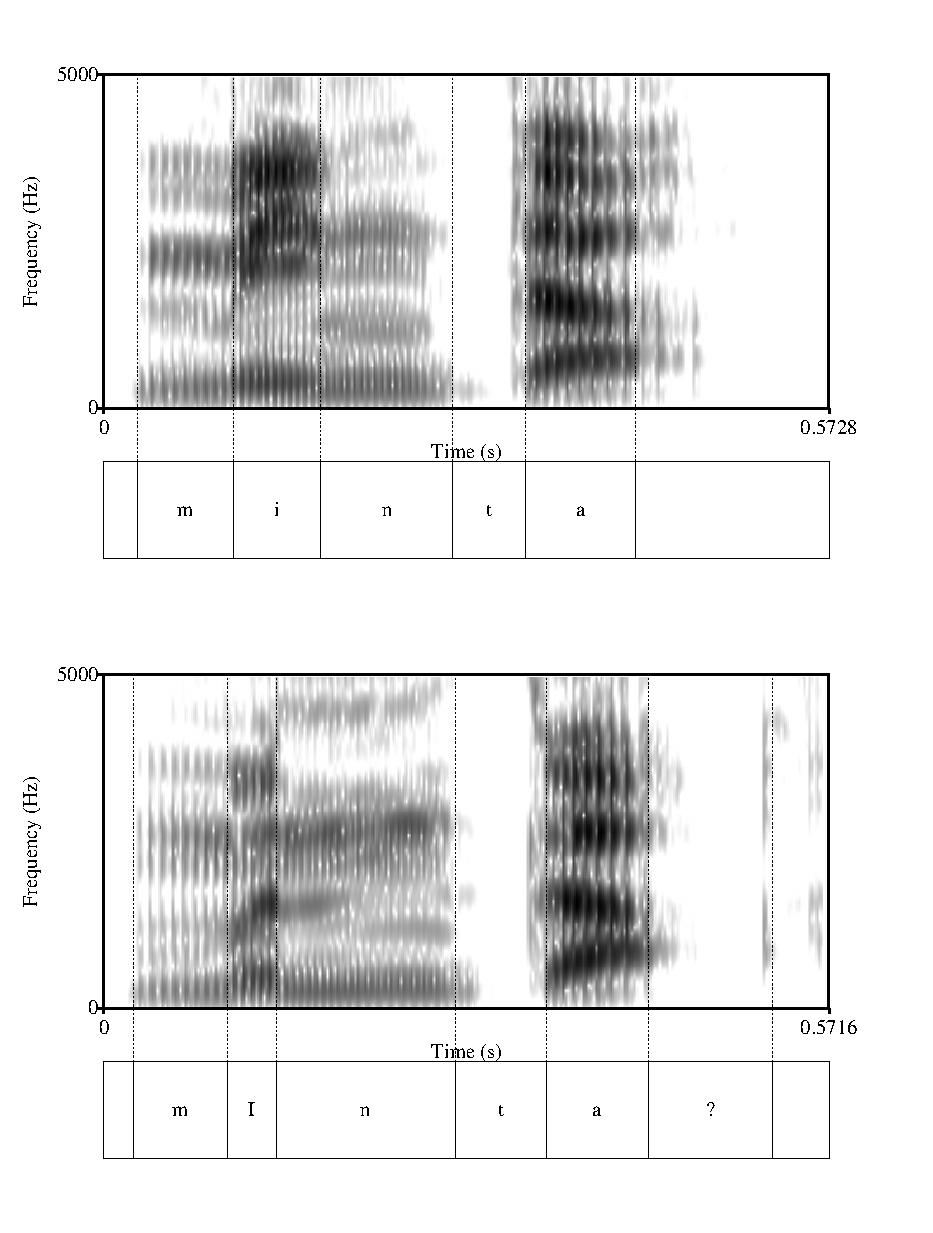
\includegraphics[width=.8\textwidth]{pics/minthamEntha.eps}
 % mentaminta.eps: 32x24 pixel, 0dpi, 70819821227670020548853019185250304.00x53114867158692554697020039288061952.00 cm, bb=
\caption[Formant structures for \phonet{I} and \phonet{i}]{The formant structures of the first vowels in \phontrs{mi\dentn\dentt a}{ask} and \phontrs{mI\dentn\dentt a}{raw} are clearly different, indicating that /i/ and /\E/ are different phonemes, which distinguish the two meanings. The second spectrogram indicates a glottal stop after the final vowel. This is not phonemic, as will be discussed in more detail below (Section \ref{sec:phon:Consonants}). }
\label{fig:minthamEntha}
\end{figure}



% The different realizations of schwa are discussed in more detail below (Section \ref{sec:phon:Majorallophonesofschwa}).



\subsubsection{Major  allophones of the full vowels}\label{sec:phon:Majorallophonesofthefullvowels}
The vowels /a/ /i/ and /u/ are always realized as full vowels. /e/ and /o/ can be realized as lax  \phonet{E,O} or tense \phonet{e,o}. Tense realizations are more often found in open syllables.

% \begin{figure}
% 	\centering
% 		\vspace{6cm}\includegraphics{pics/seelong.eps}\vspace{0.5cm}
% 	\caption{The first occurrence of the word for ``Ceylon'' is with a tense [e] the second one with a lax [\ipaE]}
% 	\label{fig:phon:seelong}
% 	%K051222nar04
% \end{figure}



 In  some words, the pronunciation of /e/ approximates the pronunciation of /i/ in the same contexts, e.g. /\dentt ekus/, `mouse',\footnote{Vowel length is not phonemic, as will be discussed in Section \ref{sec:phon:Vowellength} and therefore not indicated in the phonemic notation.}  is pronounced as [\dentt\textlowering{i}:kus].


\subsubsection{Major  allophones of schwa}\label{sec:phon:Majorallophonesofschwa}
The realization of schwa depends on its position within the stem and on the individual speaker. Schwa can be realized as \phonet{I,@,U}, and sometimes even as \phonet{i,u} (cf. \citet[27f]{Adelaar1991}, \citet{SmithEtAl2004}).


\paragraph{Variations in height}
In the final syllable, schwa is realized as \phonet{@} or \phonet{a}, depending on the speaker. In the penultimate syllable, schwa is raised by all speakers (e.g. \phontrs{bIs:aR}{big}). The amount of raising depends on the speakers. Some speakers raise to \phonet{I} or \phonet{U}, which makes the identification of the sound as a centralized vowel easy. Other speakers raise the vowel further, to \phonet{i} or \phonet{u}. In that case, the question  whether the sound is underlyingly schwa or a full vowel can only be answered by looking at word structure (see Section \ref{sec:phon:Analysisofwordstructure}). Especially a following geminate is indicative of the sound being schwa on the phonological level. In the antepenultimate and before, schwa is always realized as \phonet{@}. An example is \phontrs{c@ca\V ak}{wash}.\footnote{The normal word for `to wash' is \phonet{cu:ci}; `to bathe' is \phonet{man\postalvd i}. \phonet{c@ca\V ak} refers to an activity known in Sri Lanka as `body-wash'. This reflects the etymology of \trs{*cuci+awak}{body+wash}. I will use `wash' in the gloss as a shorthand.}

No trisyllable can have \phonet{I,U} in the initial syllable. A first set of trisyllables bans raising altogether in the initial syllable, while a second set requires raising to \phonet{i,u}. Neither set admits alternation between schwa and a high vowel. Examples for the first set are
\phontrs{c@ca:\V ak}{body wash},
\phontrs{b@Rna:ma}{famous},
\phontrs{m(@)la:ju}{Malay}, while an example for the second set is \phonem{k\E mare\ng} $\to$ \phonet{kuma:Re\ng} `yesterday'.

Since no reduced vowel is possible in the second set, contrary to the disyllables like \phontrs{\dentt\{\U/u\}l:Or}{egg},  the question arises why a schwa should be present in the underlying form. The reasons for this have to do with syllable structure and the lengthening of the vowel and will be discussed in more detail in Section \ref{sec:phon:Analysisofwordstructure}.


The verbal prefixes \phontrs{aR\E-}{\textsc{non.past}},\footnote{The semantics of this prefix are more complicated than what can be capture in the gloss here, the reader is referred to Section \ref{sec:morph:ara-} for a more thorough discussion of this prefix.}
\phontrs{an\E-}{\textsc{past}} and \phontrs{m\E-}{\textsc{inf-}}\footnote{And some other much less common prefixes, see Section \ref{sec:morph:Prefixes}.} have an unraised schwa [\E] irrespective of the syllable position. Given that most roots are disyllabic,  schwa is normally in antepenultimate position as in \phontrs{aR\E-ma:ka\ng}{is eating}, \phontrs{an\E-mi:nu\ng}{drank}, \phontrs{m\E-\J a:la\ng}{to go}, but it can also be found farther away from the end, as in \phontrs{aR\E-c\E ca:\V ak}{is washing}.  There is only one monosyllabic verbal root \phontrs{pi:}{go}. The prefixes keep the schwa unraised when combined with this root, even if this results in \phonet{\E} being in penultimate position (where normally only \phonet{I} or \phonet{U} are found): \phonet{aR\E-pi:, an\E-pi:, m\E-pi:,*aRI-pi:, *anI-pi:, mI-pi:}. Evidence from vowel lengthening suggests that these prefixes do not form one phonological word with the verb. This means that the realization of schwa in these prefixes is independent of the structure of the verb the prefixes attach to.



\paragraph{Fronting and retracting}\label{sec:phon:allophonesofschwa:frontingandretracting}

Whether schwa is raised to a front vowel \phonet{I,i} or to a back vowel \phonet{U,u}  seems to be lexically determined, but there are some phonological cues. Some lexemes only admit a front vowel, some only a back vowel, some accept both. The following list gives examples.

\ea \phonem{@mpa\dentt} `four' $\to$\phonet{Umpa\dentt}. Further raise:  \phonet{umpa\dentt}\z
\ea \phonem{g@lap} `dark' $\to$\phonet{gIl:ap}. Further raise:  \phonet{gil:ap}\z
\ea \phonem{\dentt@lOr} `egg' $\to$\phonet{\dentt Il:OR} or \phonet{\dentt Ul:OR}. Further raise:  \phonet{\dentt il:OR} or \phonet{\dentt ul:OR}\z
\ea \phonem{p@laN} `slow' $\to$\phonet{pIl:aN} or \phonet{pUl:aN}. Further raise:  \phonet{pil:aN} or \phonet{pul:aN}\z

From this list and additional material it appears that two factors have an influence: the following consonant and vowel harmony. A back vowel is most often found before a labial consonant /p,b,m/
\phontrs{d\U p:a\ng}{front},
\phontrs{k\U b:o\ng}{garden},
\phontrs{\U m:a}{mother} \citep[cf. ][27]{Adelaar1991}. Dorsal consonants seem to favor a front vowel:
\phontrs{sIg:aR}{healthy},
\phontrs{dIk:a\dentt}{vicinity}.\footnote{For theoretical discussions of this, see \citet{Clements1990sonority} and \citet[99]{Botma2004}.}
For the other consonants, a clear pattern could not be found.

\citet{Bichsel} found vowel harmony in words like \phontrs{lib:i}{more} and \phontrs{g\U m:uk}{fat} \citep[also cf.][27]{Adelaar1991}.
The schwa in the initial syllable is raised and agrees in the feature [$\pm$back] with the following vowel.

All this being said, there seems to be a lot of variation between and even within dialects. In the text K060103rec02 for example, the word for `raw' was transcribed by a native speaker once as \graphem{mintha} and two sentences later as \graphem{muntha}. Notwithstanding the intended and actual realization by the speaker, this proves that for the hearer/transcriber in this case, both the rendering of the first vowel as \graphem{i} and as \graphem{u} were acceptable, suggesting that the phonological knowledge of the hearer has no strict distinction between the fronted and the retracted realization.



\paragraph{Deletion}\label{sec:phon:schwa:deletion}
In the initial syllable of di- and trisyllables, schwa is often dropped if the resulting sequence is phonotactically acceptable.\footnote{Jakarta varieties of Indonesian show frequent deletion of schwa in initial position (Uri Tadmor p.c., \citet[229]{Ewing2005}) Many of the Sri Lankan Malays came from/through Jakarta, so that this could very well be an inherited feature.} An example for this is \phonet{m(@)la:ju} `Malay', which is rarely heard with the schwa pronounced; it is much more common to have the sequence \em ml \em as the onset of the first syllable (\phonet{mla:.ju}). Schwa is not dropped in \phontrs{c@ca:wak}{wash} and \phontrs{b@Rna:ma}{famous} because the sequences \em \#cc(c\textipa{:}) \em and \em \#brn \em are not acceptable phonotactically. Deletion of schwa is also found in disyllables,  such as \phonem{b@ras}`rice', which can be realized as \phonet{br:as}, next to \phonet{bIr:as}.\footnote{The realization with \phonet{i} is never found for this lexeme.} This reduction of schwa can also take place if no onset is present: \phonem{@ma}`mother' can be realized as \phonet{Um:a}, \phonet{um:a}, or  \phonet{\s{m}ma} with a syllabic nasal.

Realizations like \phonet{b(I)r:as}`rice' or \phonet{p(I)r:a\ng}`war' raise the question whether schwa is present in the phonological form, and then deleted, or whether it is absent in the phonological form and then  epenthetically inserted.\footnote{Tamil for instance has epenthetical insertion of \phonet{I} in onset clusters like \trs{viyaaparam}{business}$<$Skrt. \em vyaabhara \em \citep[103]{AnnamalaiEtAl1998}.} There are two reasons to prefer the deletion account over the epenthesis account. First, there is a phoneme schwa anyway, so the presence of schwa in this position is no additional burden. Second, schwa varies with \zero{} only in some contexts, in lexemes like \phontrs{c\E ca:\V ak}{wash}, \zero{} is not possible. An epenthetic account can thus not explain the whole story, while the deletion account can. Additionally, schwa is the historical vowel in these words, although the speakers are of course not necessarily aware of this.



\subsubsection{Vowel length}\label{sec:phon:Vowellength}
Full vowels are predictably lengthened in open penultimate syllables.  Long vowels are not found in other positions. Vowel length is thus not phonemic (\em contra \em \citet{Bichsel, SmithEtAl2004}), but conditioned by nature and position of the syllable \citep[cf.][]{Tapovanaye1995}. Example \xref{ex:phon:vowellength} shows this lengthening process for all full vowels.


\xbox{14}{
\ea \label{ex:phon:vowellength}
\gll ma:Ra --- me:Ra --- \postalvd i:Ri --- so:Re --- mu:Ra  \\
      anger --- red --- body --- evening --- cheap \\
\z
} \\

Example \xref{ex:phon:vowellength} contains only disyllabic words.
In trisyllabic words with an open penultimate syllable, the syllable is lengthened if the initial syllable contains a schwa \xref{ex:phon:vowellength:trisyl:schwa} in any of its realizations (\phonet{@,I,i,U,u}). It is not lengthened otherwise \xref{ex:phon:vowellength:trisyl:noschwa}.\footnote{There are close to no underived stems without schwa in the initial syllable. I analyze \phontrs{nigiri}{country} and \phontrs{ku\dentt umuN}{see} as having no schwa synchronically in spite of the diachronic origins \em n\E g\E ri \em and \em k\E t\E mu \em because the vowels are always pronounced as full vowels, and none of the other phonological effects of schwa are found. As far as trisyllabic words derived with affixes go (like \em makan-an\em), all have only short vowels.}


\xbox{14}{
\ea \label{ex:phon:vowellength:trisyl:schwa}
\gll c\E ca:\V ak --- m\E la:ju  --- kuma:Re\ng   \\
      wash  ---  Malay ---  yesterday\\
\z
} 


\xbox{14}{
\ea\label{ex:phon:vowellength:trisyl:noschwa}
\gll nigiRi ---  ku\dentt umu\ng{} ---  makanan \\
     country  --- see ---  food  \\
\z
} \\

No surface form of an underlying schwa (\phonet{@,I,i,U,u}) is ever lengthened. Instead, often another phonological process, consonant gemination, takes place, see Section \ref{sec:phon:Analysisofwordstructure}.

This general pattern is very regular throughout the grammar, but a certain number of exceptions apply:

\begin{itemize}
 \item function words never have long vowels: \phontrs{ki(*:)\dentt am}{\textsc{1pl}}, \phontrs{ka(*:)\dentt a}{\textsc{quot}}, with the exception of interrogative pronouns.
\item the sequence V$_i$hV$_i$ never has a long vowel: \phontrs{le(*:)heR}{neck}, but \phontrs{la*(:)heR}{be.born}
\item some sequences VGV, where G is a glide, have a long vowel, others do not. \phontrs{\dentt u*(:)\V a}{old}, \phontrs{\dentt u(*:)\V an}{Sir}. See Section \ref{sec:phon:nonphonemicglideformation} for detailed discussion.
\item the sequence \em uru \em has no long vowel in the words \phontrs{\dentt uRus}{straight}  and \phontrs{guRu}{teacher} (but there is a long vowel in  \phontrs{ku:Rus}{thin}).
\item two words are lexical exceptions \phontrs{kubu:R}{bury}{} and \phontrs{ka:R\dentt u}{quarter}. The former has a long vowel in the final, not the penultimate, syllable. The latter has a long vowel in the penultimate syllable, but the syllable is not open.
\item Loanwords from English and Arabic tend to violate this pattern.
\end{itemize}


 

\subsubsection{Distribution of the vowels}\label{sec:phon:Distributionofthevowels}
For the discussion of the distribution of vowels, we distinguish the root level from the stem level. In the context of this discussion, roots are defined as monomorphemic lexemes, while stems consist of at least one root and optional additional morphemes, lexical or derivational. To illustrate the distinction with English examples, \em farm \em would be a root,\footnote{And also a stem.} whereas \em dairy farm \em or \em farmer \em would be stems, because they comprise additional morphemes, \em dairy \em and \em -er \em in these cases.

In SLM roots, there are no restrictions for the final and the penultimate syllable. Here, all vowels can be found. Examples are given in Table \ref{tab:vowelpositions}. In the antepenultimate position, only [i], [u] and [\E] are found in native roots. Any vowel can be found in the antepenultimate position in loanwords, which are given in parentheses in Table \ref{tab:vowelpositions}.

\begin{table}
	\begin{center}
		\begin{tabular}{llll}
		& antepenultimate& penultimate & final \\
		\hline
		a & (\textipa{va\tz:ak:a:}`pumpkin', Tamil)	& \textipa{\dentt aksiR} `think'	& \textipa{kap:al} `ship' \\
		e & (\textipa{selin\postalvd i}`{spider}', Tamil)	& \textipa{seksa} `problem' 	& \textipa{slampe} `handkerchief'\\
		i & \textipa{nigiRi}`country'	& \textipa{mi\dentn\dentt a} `ask'& \textipa{sampi} `cow'\\
		o & (\textipa{goRaka:}`a condiment' Sinhala)	& \textipa{pompa\ng} `female'	& \textipa{na\dentn\dentt ok} `sleepy' \\
		u & \textipa{ku\dentt umu\ng}`see'	& \textipa{kumba\ng} `flower'&	 \textipa{campuR} `mix'\\
		schwa & \textipa{c\E ca\V ak} `wash'	& \textipa{mI\dentn\dentt a} `vomit'	& ka\dentt:\E m `almsgiving'\\
		\end{tabular}
		\caption[Vowels in different positions within the root]{Vowels in antepenultimate, penultimate and final position of roots. In antepenultimate position, a, e and o are only found in loanwords, indicated by parentheses. The word \trs{bahasa}{language} could be an exception, but this seems to be a recent borrowing from Standard Malay, the native word is \phonet{ba:sa}.}
		\label{tab:vowelpositions}
	\end{center}
\end{table}

As for stems, no such restrictions apply. When adding the nominalizing suffix \em -an \em to a verbal root, the penultimate becomes the antepenultimate and keeps its vowel. In this way, [e], [o] and [a] can be found in the antepenultimate, e.g. \phontrs{pake-yan}{dress\textsc{-nmlzr}},\phontrs{po\dentt o\ng-an}{cut-\textsc{nmlzr}}, \phontrs{pegan- an}{catch-\textsc{nmlzr}}. Similar things can be said about compounding, which also shifts syllables farther away from the right edge. This does not affect the occurrence of [e], [o] or  [a] either. Examples are \phontrs{oRa\ng{} ik:a\ng}{man+fish=fisherman}  and \phontrs{babi u:\dentt a\ng}{pig+forest=wild boar}.

While schwa can occur anywhere, it is most often found in the penultimate and the antepenultimate. There are only two occurrences of schwa in the final syllable of two words, which are given below

\xbox{7}{
\ea\label{ex:phon:schwafin:thaanEm} 
\gll \dentt a:n\E{}m\footnotemark{} \\
    `plant(V)' \\
\z
}
\xbox{7}{
\ea
\gll ka\dentt:\E m \\
    `almsgiving' \\
\z
}
\footnotetext{While Std. Malay does not permit schwa in the final syllable, Jakartanese does \citep{AdelaarEtAl1996}, and \em tan\E m \em is also found in that variety, with the same meaning \citep[200]{Adelaar1985}.}

\subsection{Consonants}\label{sec:phon:Consonants}
SLM numbers 24 native consonants and glides plus 3 consonants only used for loanwords. 5 basic places of articulation are distinguished for stops: labial, dental, apical (with postalveolar and retroflex allophones),\footnote{I use `apical' as a cover term for  postalveolar and retroflex realizations. This term as it is used here never includes the dentals, no matter how they are realized.} palatal, and velar. These places have a series of voiceless stops, voiced stops and prenasalized voiced stops.\footnote{The dental prenasalized stop is missing.} The palatal stops are realized as affricates (For the general treatment of affricates as strident stops see \citet{JakobsonEtAl1952speechanalysis,Clements1999affr}, and \citet{Kehrein2002affr}.
% \footnote{As is the case with most other languages on the subcontinent,  languages which have palatal affricates do not have palatal stops. \citep[67]{Ramaswami1999}.}

All stops are matched by homorganic nasals, with the exception of the lamino-dental nasal, which does occur phonetically, but lacks phonemic status.

The fricative series is less populated, with /s/ being the only fricative frequently encountered. There are some words with /h/, but overall /h/ is much less frequent than /s/. /f/, /z/ and /\sh/ are finally only found in loanwords from Arabic (\phontrs{zihaRa\dentt}{shrine}) or English (\phontrs{femili}{family}, \phontrs{bRItIS}{British}). /f/ and /z/ are also found in many Islamic names like \em Farzan \em or \em Fayizal\em.

/l/ is an alveolar lateral approximant. /r/ is a rhotic realized as a tap or a trill.

The picture is completed by a labiodental approximant \V{} and a palatal approximant \textipa{j} (cf. Table \ref{tab:SLMConsonantPhonemes}).

\begin{table}
    \centering
        \begin{tabular}{lcccccc}
                 & labial & dental & apical    & palatal          & velar & glottal\\
        \hline
        stops    &&&&&&\\
        ~~~voiceless& p   & \dentt{} & t        &    c        & k   &   \\
        ~~~voiced   & b   & \dentd{} & d        &   \J          & g   &   \\
	~~~prenasalized&\mb& 	     & \nd         &  \nJ        & \nG &   \\
	nasals      & m   &         &  n           & \ny	  & \ng &   \\
       fricatives  & (f) &          &    s (z) (\textesh)    &   &     & h \\
	 approximants & \V  &          &       &   j         &     &   \\
	 liquids &   &          &  r ~~ l      &            &     &   \\
        \end{tabular}
    \caption[SLM consonant phonemes]{SLM consonant phonemes, including approximants. Palatal stops are phonetically affricated. Parentheses indicate phonemes only found in loanwords.}
    \label{tab:SLMConsonantPhonemes}
\end{table}
% 
% 
% \begin{figure}
% 	\centering
% 	\subfigure[Sinhala consonant phonemes. Palatal stops are phonetically affricated.]{
%     \centering
%         \begin{tabular}{lcccccc}
%                  & labial & dental & retroflex    & palatal          & velar & glottal\\
%         \hline
%         stops    &&&&&&\\
%         ~~~voiceless& p   & \dentt{} & \tz        &   c         & k   &   \\
%         ~~~voiced   & b   & \dentd{} & \dz        &   \J           & g   &   \\
% 	~~~prenasalized&\mb&\ndentd      & \nd         &           & \nG &   \\
% 	nasals      & m   &         &   n            & \ny	  & \ng &   \\
%         fricatives  & (f) &          &    s (z)(\textesh)     &   &     & h \\
% 	other & \V  &          &  r ~~ l      &   j         &     &   \\
%         \end{tabular}
% 	}        
% 	\subfigure[Sri Lanka Muslim Tamil consonant phonemes.  Palatal stops are phonetically affricated. Sounds in brackets are not phonemic in all dialects of Tamil.]{
%     \centering
%         \begin{tabular}{lcccccc}
%                  & labial & dental & apical    & palatal          & velar & glottal\\
%         \hline
%         stops    		& p   & \dentt{} & [\underline{t}] t{}        &   c(\J)          & k   &   \\
%         nasals      & m   & n        &   \nz           & \ny	  & \ng &   \\
%         fricatives  &  &          &    (s)     & (\textesh)  &     & (h) \\
% 	other & \V  &          &  r ~~ l ~~ \lz{} ~~ [\zz]    &   j         &     &   \\
%         \end{tabular}
% 	}        
% 	\caption{Consonant inventories in the adstrates. Parentheses indicate phonemes only found in loanwords.}
%   \label{tab:AdstrateConsonants}
% \end{figure}


\citet{Bichsel} and \citet{Adelaar1991} concur with this inventory, but do not list the prenasalized series, while \citet{SmithEtAl2004} express doubts about the apical series, and do not list the prenasalized series either. Minimal pairs establishing both apical as a place of articulation and prenasalized stop as a manner are given below.

\begin{figure}
	\centering
		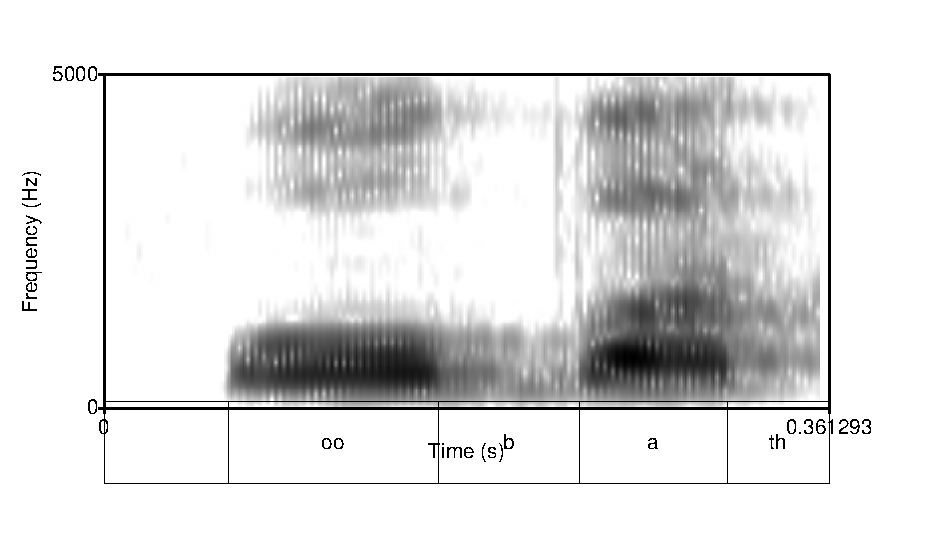
\includegraphics{pics/oobath.eps}
	\caption[Absence of a glottal stop before vocalic onset]{No glottal stop is found before the word initial [o:] in \phontrs{o:ba\dentt}{medicine}}
	\label{fig:phon:oobath}
	%K051222nar04
\end{figure}

\citet{Tapovanaye1995} finds glottal stops  before initial vowels and after final vowels, but does not grant them phoneme status.
\citet{Bichsel} found a glottal stop before every initial vowel. For reasons of syllable structure, she granted phoneme status to it. She wanted to eliminate syllables without onset.  In my data, the glottal stop is clearly optional.  Figure \ref{fig:minthamEntha} shows a glottal stop. While it is tempting to treat this as a reflex of historical \phontrs{*m\E ntah}{raw} as opposed to historical \phontrs{*minta}{beg}, the occurrence of the glottal stop is too irregular between speakers and lexemes to establish a clear correlation pattern between historical /h\#/ and the occurrence of the glottal stop in the modern language.
There is variation as to whether the glottal stop occurs word-initially, \phonet{Pa:nak} or \phonet{a:nak} `child'. Word-medial but syllable-initial vowels do not get a glottal stop preposed (\phonet{\J a:u}`far', not *\phonet{\J a:Pu}). The differences between the data of the aforementioned authors and my data might be due to the fact that they worked with elicited lexemes, while the data this analysis is based on  naturalistic speech. In the context of an elicitation session (like the one which yielded the data for the spectrogram in Figure \ref{fig:minthamEntha}), a glottal stop is often inserted in citation forms of words before an initial vowel and after a final vowel. This glottal stop insertion is not very regular in non-citation contexts. \citet{Bichsel} and \citet{Tapovanaye1995} treat it as a regular process, but this is not supported by the data in my corpus.  Vowels in initial position are frequently found without glottal stop. As an example, the word \phontrs{o:ba\dentt}{medicine}, pronounced after a pause of about 0.7 seconds (not  represented completely in the graphic), does not receive a glottal stop, as can be seen from Figure \ref{fig:phon:oobath}.

In this description, I therefore do not assume a phonemic glottal stop. 

\subsubsection{Distinctions in place of articulation}\label{sec:phon:Distinctionsinplaceofarticulation}
This section provides minimal pairs for all possible pairs of two neighboring places of articulation.

\paragraph{Stops}
Distinctive places of articulation for stops are:  labial, dental, apical, palatal, and velar. Apical comprises postalveolar and retroflex allophones. Apical as it is used in this description never comprises dental stops. In phonemic representation, /t/ will be used for apical stops, while the allophones will be represented as \phonet{\postalvt,\postalvd} and \phonet{\tz,\dz}.\\

\xbox{6}{
/p/ \textbf{vs.} /\dentt/
\ea
\gll  \textipa{ba:pa}  --- \textipa{ma:\dentt:a} \\
      father --- eye \\
\z      
}
\xbox{6}{
/b/ \textbf{vs.} /\dentd/
\ea
\gll  \textipa{ba\dentt a ba:\dentt a}  --- \textipa{\dentd a:\dentt ang} \\
      bricks --- come \\
\z      
}
\xbox{6}{
/\mb/ \textbf{vs.} /\ndentd/
 
n/a
     
}

\xbox{6}{
/\dentt/ \textbf{vs.} /t/
\ea
\gll  \textipa{kO:\dentt OR}  --- \textipa{kO:\tz OR} \\
      dirt --- fool \\
\z      
}
\xbox{6}{
/\dentd/ \textbf{vs.} /d/
\ea
\gll  \textipa{\dentd u:a}  --- \textipa{\dz u:\V a} \\
      praise --- two \\
\z      
}
\xbox{6}{
/\ndentd/ \textbf{vs.} /\ndz/
 
n/a
 
}

\xbox{6}{
/t/ \textbf{vs.} /c/
\ea
\gll  \textipa{kO:\tz OR}  --- \textipa{cO:cO} \\
      fool --- kind.of.fruit \\
\z      
}
\xbox{6}{
/d/ \textbf{vs.} /\J/
\ea
\gll  \textipa{a:\dz a}  --- \textipa{a:\J aR} \\
      exist --- teach \\
\z      
}
\xbox{6}{
/\ndz/ \textbf{vs.} /\nJ/
\ea
\gll  \textipa{\dentt a:\ndz ak} --- \textipa{pa:\nJ aN} \\
      dance --- long \\
\z
}

\xbox{6}{
/c/ \textbf{vs.} /k/
\ea
\gll  \textipa{cu:ci}  --- \textipa{ku:ciN} \\
      wash --- cat \\
\z      
}
\xbox{6}{
/\J/ \textbf{vs.} /g/
\ea
\gll  \textipa{\J a:ga}  --- \textipa{ga:\J a} \\
      protect --- elephant \\
\z      
}
\xbox{6}{
/\nJ/ \textbf{vs.} /\nG/
\ea
\gll   \textipa{pa:\nJ aN}   --- \textipa{ma:\nG a} \\
      long --- mango \\
\z
}





\paragraph{Fricatives}
There are only two native fricatives, /s/ and /h/, for which example \xref{ex:phon:min:sh} provides a near minimal pair. In Tamil \phonet{s} and \phonet{c} are allophones of /c/ ({\btam \TAMc \etam}) \citep[174]{Suseendirarajah1973phon}.
 Therefore it is necessary to establish that these phonemes are indeed different in SLM. Examples \xref{ex:phon:min:stsh} shows this. For the sake of completeness, example  \xref{ex:phon:min:sdzh} proves that /s/ is  also different from /\J/. /\sh/ and /z/ are only found in loanwords.\\

\xbox{5}{
/s/ \textbf{vs.} /h/
\ea\label{ex:phon:min:sh}
\gll  \textipa{kO:sON}  --- \textipa{pOhON} \\
     empty --- tree \\
\z      
}
\xbox{5}{
/s/ \textbf{vs.} /c/
\ea\label{ex:phon:min:stsh}
\gll  \textipa{ba:sa}  --- \textipa{ba:ca} \\
      wet --- read \\
\z      
}
\xbox{5}{
/s/ \textbf{vs.} /\J/
\ea\label{ex:phon:min:sdzh}
\gll  \textipa{ba:sa}  --- \textipa{bla:\J aR} \\
       wet --- learn \\
\z      
}

/f/ is marginally phonemic and is found in a few words or Arabic origin, like \phontrs{fi\dentt ena}{slander} and \phontrs{kafan}{shroud}, besides proper names and religious terms.


\paragraph{Nasals} The following list provides minimal pairs for all pairs of neighbouring nasals. Note that there is no dental nasal phoneme,\footnote{\phonet{\textsubbridge{n}} does occur before dental stops, but this is always the result of assimilation.} hence /m/ and /n/ are neighbours.\\

\xbox{14}{
/m/ \textbf{vs.} /n/ \textbf{vs.} /\ny/ \textbf{vs.} /\ng/
\ea
\gll  \textipa{\dentt a:ma}  --- \textipa{\dentt a:na} --- \textipa{\dentt a:\ny a}  --- \textipa{\dentt a:NaN}\\
      before --- soil ---  ask --- hand                                 \\
\z      
}\\
% \xbox{5}{
% /n/ \textbf{vs.} /\ny/
% \ea
% \gll  \textipa{O:nE\dentt}  --- \textipa{m^wO\ny E\dentt} \\
%       creeper --- monkey \\
% \z
% }
 
\paragraph{Glides}
SLM has two glides, /\V/ and /j/. These are distinctive as the following examples show.\\

\xbox{7}{
/\V/ \textbf{vs.} /j/
\ea\label{ex:phon:min:w}
\gll sa:\V a --- sa:ja\ng \\
      fields  --- love  \\
\z      
}

\paragraph{Phonemic status of the glides}\label{sec:phon:nonphonemicglideformation}
Some occurrences of the glides, like those in \xref{ex:phon:min:w}, are clearly phonemic and present in the underlying form. Other occurrences could be the result of a phonological constraint banning hiatus, especially when a long vowel is involved. This is schematized in \xref{ex:phon:glide:threemorae} \citep[cf.][23]{Tapovanaye1995}.

\ea\label{ex:phon:glide:threemorae} CV$_i$.V$_j\to$CV$_i$\textipa{:}V$_j\to$CV$_i$GV$_j$\z

or, in a more formal way

\ea\label{ex:phon:glide:threemorae:formal} $[+vocalic][+vocalic]\to[+vocalic][-vocalic]/\_[+vocalic]$ \z

The second vowel in a two-vowel sequence is not realized as vocalic in front of a third vowel. Evidence for this comes from the absence of a long vowel in environments which would normally require one (Section \ref{sec:phon:Vowellength}, p. \pageref{sec:phon:Vowellength}). An example is \phontrs{lija\dentt}{see}, where we would normally expect \phonet{li:a\dentt} or \phonet{li:ja\dentt} with a long vowel. This problem of the missing long vowel can be solved if we assume that the sequence VG is a special realization of a long vowel.
It would then appear that the second part of the vowel is turned into a glide, leaving only the first part as vocalic and thus resulting in a short vowel.
Next to /i/, this is found for /u/, for example in \phontrs{bu\V aN}{throw}, where the right part of the long /u/ is turned into a glide.
% Some evidence for this can be found in a transcript made by a native speaker (K051205nar05), who wrote the word for `to get up' once with a long vowel (\em baaung\em), and once with a short vowel followed by a glide (\em bavung\em).

If the first vowel is neither /i/ nor /u/, the glide formation is not found, resulting in hiatus as in \phontrs{\J a:u}{far}.\footnote{The phonological conditions of a preceding high vowel in order to form a glide are actually a common feature of Austronesian languages \citep[116]{Himmelmann2005typochar}.} In these cases, a long vowel is always found. Also note that a short vowel in the penultimate syllable of  disyllabic words is only possible if the onset of the final syllable is a glide. This distribution strongly suggests that [ij] and [u\V] are alternative realizations of a lengthened /i/ and a lengthened /u/.

The analysis of the creation of a sequence VG out of a long vowel is complicated by the fact that there are some words with a sequence V\textipa{:}G, like those given in \xref{ex:phon:min:w}. While in \xref{ex:phon:min:w}, this is not problematic because /a/ does not have a corresponding glide, there are also some words where a long [+high] vowel is followed by a glide, e.g. \phontrs{bu:\V a}{fruit}. This can be analyzed as an underlying form /bu.\V a/, which undergoes the regular vowel lengthening process of open penultimate syllables in disyllabic words. There are thus words of the type /CV.V(C)/ like \phonem{bu.aN} which have to be distinguished from words of the type /CV.GV(C)/ like \phonem{bu.\V a}.\footnote{For an  argument for the theoretical distinction between phonemic and non-phonemic glides see \citet{Levi2008glides}.}

The only other instance where a short vowel is found in the open penultimate of a disyllabic lexical word is in the sequence V$_i$hV$_i$ (e.g. \phontrs{leheR}{neck}). There might be the possibility to explain this sequence in a manner akin to the occurrence of non-phonemic glides, similar to the solution proposed by Tapovanaye (see Section  \ref{sec:phon:Problematiccases}), but this needs more theoretical research.


 
% /\dentd unia/ `world' is normally pronounced \phonet{\dentd unija}. The non-phonemic character of the glide in this word can be seen by the lack of length in the /i/.





\subsubsection{Manner and voicing distinctions}\label{sec:phon:Mannerandvoicingdistinctions}
Having discussed the different places of articulation, we now discuss the different manners of articulation available for the different places of articulation. Voicing contrasts are also discussed here for convenience.

\paragraph{Distinctions for labial consonants}
{~}\\

\xbox{14}{
/p/ \textbf{vs.} /b/ \textbf{vs.} /m/ \textbf{vs.} /\V/
\ea
\gll  \textipa{sa:pa}  --- \textipa{Ra:ba} --- \textipa{sa:ma} --- sa:\V a\\
       who? --- caress  --- together --- fields\\
\z      
}\\ 

\paragraph{Distinctions for coronal consonants}

{~}\\
\xbox{14}{
/\dentt/   \textbf{vs.} /s/ \textbf{vs.} /n/ \textbf{vs.} /r/ \textbf{vs.} /l/
\ea
\gll  \textipa{ga:\dentt al}    --- \textipa{Ra:sa} 	--- \dentt a:na --- \dz a:\textipa{R}a --- sa:la \\
      itch 			---  tasty 		--- soil --- blood --- wrong\\
\z      
}\\

\xbox{14}{
/\dentt/ \textbf{vs.} /t/ \textbf{vs.} /d/  \textbf{vs.} /s/ \textbf{vs.} /n/ \textbf{vs.} /r/ \textbf{vs.} /l/
\ea
\gll   \textipa{ku:\dentt u} --- \textipa{lu:\tz u\dentt}  --- \textipa{\dz u:\dz uk} --- su:su --- gu:nu\ng{} --- \textipa{\dentt u:RuN} --- \textipa{spu:lu} \\
      louse --  knee --- sit --- milk --- mountain --- get.down --- ten \\
\z      
}\\


\xbox{14}{
/\dentd/ \textbf{vs.} /d/ \textbf{vs.} /\dentt/
\ea
\gll \textipa{\dentd u:a} --- \textipa{\dz u:\V a} --- \textipa{\dentt u:\V a}   ~~~~{\rm apical /t/ is not possible initial position} \\
      recital --- two --- old \\

\z
} \\


\xbox{14}{
/\dentt/ \textbf{vs.} /t/ \textbf{vs.} /d/
\ea
\gll \textipa{kO:\dentt OR} --- \textipa{kO:\tz OR} --- \textipa{kO:\dz Ok}   \\
      dirt --- fool --- frog \\
\z
} \\


\xbox{14}{
/\dentd/ \textbf{vs.}  /d/
\ea
\gll pa\dentd eRi --- a:\postalvd e \\
     struggling --- younger.sibling  \\
\z
} \\


\xbox{14}{
\phonet{\textsubplus{\:r}} (allophone of /d/) \textbf{vs.} \phonet{R} (allophone of /r/)
\ea
\gll \rm{\textipa{\dz a:\textsubplus{\:r}a}} --- \rm{\textipa{\dz a:Ra}}\\
       chest --- blood\\
\z      
}\\



\paragraph{Distinctions for palatal consonants}
{~}\\

\xbox{7}{
/c/ \textbf{vs.} /\J/ \textbf{vs.} /\ny/
\ea
\gll  \textipa{ca:Ri}  --- \textipa{\J a:\postalvd i} --- \textipa{\ny a:\ny i} \\
       find --- become --- sing\\
\z      
}\\ 

\paragraph{Distinctions for velar consonants}
{~}\\

\xbox{7}{
/k/ \textbf{vs.} /g/ \textbf{vs.} /\ng/
\ea
\gll  \textipa{kla:ki}  --- \textipa{\dz a:giN} --- \textipa{a:NiN}  \\
       boy --- beef --- air \\
\z      
}\\ 




\subsubsection{The prenasalized stops}\label{sec:phon:Theprenasalizedstops}

\begin{figure}
 \centering 
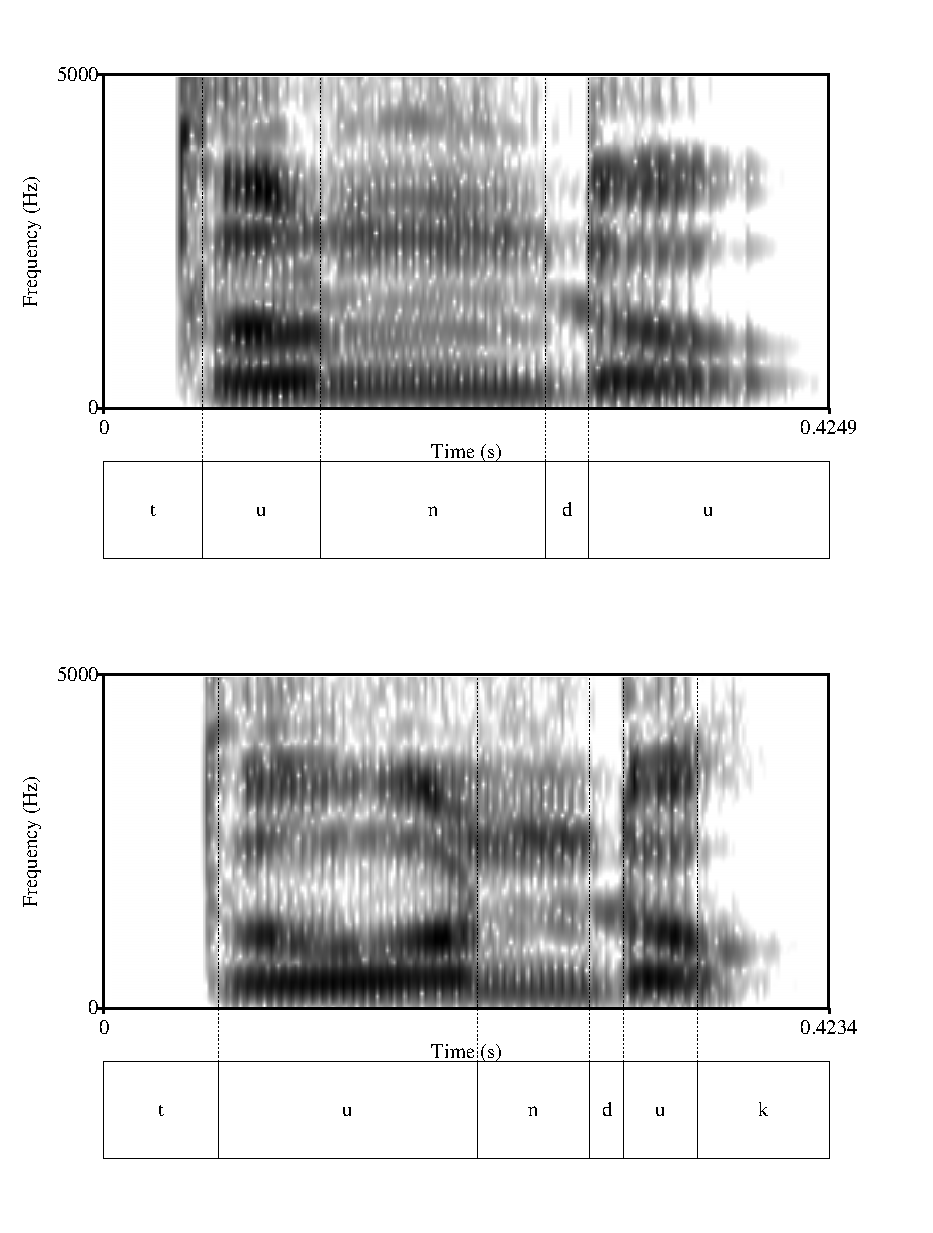
\includegraphics[width=.8\textwidth]{pics/thunduthuunduk.eps}
%  Spectrogram-non-prenasalized-consonant.png: 432x252 pixel, 72dpi, 15.24x8.89 cm, bb=0 0 432 252
\caption[Spectrogram of tautosyllabic and heterosyllabic NC-clusters]{The heterosyllabic sequence /n.d/ in the Tamil loan \phontrs{\dentt u\nz.\dz u}{piece} has a short vowel (69ms) and a comparably longer nasal (132ms) than the tautosyllabic sequence /.nd/ in the native word \phontrs{\dentt u:.\ndz uk}{bend} below (151ms+66ms). The latter sequence is analyzed as a phonemic prenasalized consonant in this grammar.}
\label{fig:thunduthuunduk}
\end{figure}

SLM has four prenasalized stops matching the points of articulation of the non-prenasalized stops. The dental prenasalized stop is not found. Prenasalized stops contrast with N+stop clusters both phonetically and phonologically. Phonetically, the prenasalized consonants have a much shorter nasal phase (Figure \ref{fig:thunduthuunduk}). Phonologically, vowels preceding prenasalized consonants are lengthened when in penultimate position of disyllabic stems (for more discussion of vowel lengthening see Section \ref{sec:phon:struct:Roots}). This suggests that the prenasalized consonants do not close the preceding syllable. N+stop clusters, on the other hand, never occur after a long vowel, suggesting that the nasal part closes the preceding syllable. This absence of vowel lengthening in heterosyllabic clusters can also be seen  in Figure \ref{fig:thunduthuunduk}, where the vowel is shorter before the N+C cluster of \phontrs{\dentt u\nz\dz u}{piece} (above), and longer before the prenasalized \nd{} in \phontrs{\dentt u:\ndz uk}{bend} below.

Both heterosyllabic and tautosyllabic NC sequences are listed in 
 Table \ref{tab:PrenasalizedConsonants}, together with some other combinations of voiced stop and/or nasal.
\begin{table}
	\begin{center}
	% use packages: array
	\begin{tabular}{ccccccc}
	 		& V\textipa{:}.CV 			& VC.CV 			& V\textipa{:}.NV 				& VN.NV   			& VN.CV					& V\textipa{:}.\super{N}CV \\
	\hline
	labial   	& \tbltrs{ba:i}{pig}		& \tbltrs{hab:aR}{news}		& \tbltrs{\dentt a:ma}{earlier}	& \tbltrs{sam:a}{every}	  	&  \parbox{2.5cm}{\centering\textipa{sambal} \\`{spicy food}'}	& \tbltrs{ga:\mb aR}{picture}\\\\
	dental   	& n/a			& n/a				& 	n/a				&  	n/a			& \tbltrs{seli\dentn\dentd i}{spider} 	& n/a 				\\\\
	apical		& \tbltrs{li:\dz a}{tongue}	& \tbltrs{pI\dz:ang}{sword}	& \tbltrs{pi:nang}{areca nut}		&  \tbltrs{bIn:ang}{thread}	& \tbltrs{\dentt u\nz\dz u}{piece} 	& \tbltrs{\dentt u:\ndz uk}{bent}  \\\\
	palatal  	& \tbltrs{ga:{\J}i}{salary}	& \tbltrs{ha\J:i}{Haj}	& \tbltrs{\ny a:\ny i}{sing}	& \tbltrs{ba\ny:ak}{much}		& \tbltrs{a\ny\J iN}{dog}		& \tbltrs{ba:\nJ iR}{flood}\\\\
	velar    	& \tbltrs{\dentt i:{g}a}{three}	& \tbltrs{sIg:aR}{healthy}	& \tbltrs{i:Na\dentt}{think} 		&  \tbltrs{\dentt IN:a}{middle}& \tbltrs{siNga}{lion}			& \tbltrs{mni:\nG al}{die} \\\\
	\hline\hline
	\end{tabular}
	\caption[Medial combinations of nasal and stop]{Prenasalized consonants in opposition to plain and geminated stops, plain and geminated nasals, and clusters of nasal+stop. Dental stops normal do not occur word-medially. \phontrs{seli\dentn\dentd i}{spider} is an exception, a loanword from Tamil.}
	\label{tab:PrenasalizedConsonants}
	\end{center}
% pa\dentn\dentd el ceremony.cloth
% tIndang kick
% piiNDa spread
\end{table}


% 
% Prenasalized stops have been proposed by \citep{Thera1986, Tapovanaye1995}. \citet{Bichsel} argues against prenasalized stops because they would increase the phoneme inventory. Other authors have remained by and large silent on this subject, but \citet{SmithEtAl2004} regard Bichsel's analysis as superior.
% Tapovanaye's analysis is based on the observation that long vowels can generally only occur in open syllables. The only exception to this are syllables closed by a nasal homorganic to the following stop, i.e. V:mbV, V:n\dentd V, V:nd V, V:\ng gV. In order to retain his rule of vowel lengthening in open syllables, Tapovanaye analyzes these sequences as V:.\mb V, V:.\ndentd V, V:.\ndz V, V:.\nG V, shifting the nasal to the onset of the following syllable. Bichsel misreads the proposal as suggesting that \mb{} and b, \ndentd{} and \dentd{} etc. would be allophones and shows convincingly that they are not, but Tapovanaye had never claimed that. Some parts of Bichsel's comments refer to the analysis which Tapovanaye intended and object that such an analysis would increase the size of the phoneme inventory by four, namely \mb, \ndentd, \ndz{} and \nG\footnote{Bichsel does not list /\ndzh/ as a phoneme, otherwise the increase would have been by five.}. This is of course true, but a phoneme inventory should contain all sounds which matter on the phonological level of analysis, and there is no need to keep the size of an inventory smaller than necessary. On phonological grounds alone, there is enough reason to accept the prenasalized stops as members of the phoneme inventory, because they allow for a straightforward explanation of vowel lengthening in open syllables, a generalization that cannot be captured otherwise. But instrumental analysis also shows that the sequences NC and \u{N}C differ phonetically. Figure \xref{fig:phon:sambalgaambar} shows  spectrograms of the word \phontrs{sambal}{sauce} and \phontrs{ga:\mb aR}{picture}. The  nasal in \em ga:\mb ar \em is clearly shorter than the nasal in \em sambal \em.

Additional support for the phonemic status of the prenasalized consonants comes from acceptability judgments. Speakers were asked whether \em sambal \em and \em ga:\mb ar \em could be written with the sequence \graphem{m+b} ({\SHa\char253}{\SHa\-\char237a}) or the prenasalized consonant \graphem{\mb} ({\SHb\char117a}) in Sinhala script. Informants generally accepted the writing \graphem{m+b} for both forms, but the writing \graphem{\mb} only for \em ga:\mb ar\em. Analogous results were obtained for words with other prenasalized consonants. This shows that these sounds are cognitively different for the speakers, otherwise they should have been treated alike. This is even more significant given that the vowel preceding a prenasalized stop tends to be reduced in Sinhala, but lengthened in SLM. Artefacts in the choice of grapheme resulting from vowel quality can therefore be excluded.

\subsubsection{The palatal obstruents}\label{sec:phon:Thepalatalobstruents}  
SLM numbers three palatal obstruents \phonem{c,\J,\nJ}, which, besides their realization as stops, have affricate allophones \phonet{\textcttctclig,\textctdctzlig,\super{\ny}\textctdctzlig}. Given that the other stops do not have the option of affrication, the question arises whether these phonemes pattern with the stops, or whether they are in a natural class of their own, the class of affricates (cf. \citet[63]{Bichsel}, \citet[357]{Noonan2006}). First, we have to establish whether they consist of one phoneme or two. In case they consist of only one phoneme, we have to answer the question whether this phoneme is internally complex.

\citet{Trubetzkoy1939} contains a list of rules how to decide between the `monophonematic' and the `polyphonematic' analysis of a certain part of the sound sequence (\em Schallstrom\em). Particularly relevant for SLM are the rules IV and VI, which are given below.

\begin{quote}
Regel IV. Eine potentiell monophonematische \el{} Lautverbindung muß als Realisation eines einzigen Phonems gewertet wetden, wenn sie als Einzelphonem behandelt wird, d.h. wenn sie in solchen Lautstellungen vorkommt, wo in der betreffenden Sprache Phonemverbindungen nicht zugelassen werden.\footnote{A potentially monophonematic sound combination must be seen as the realization of exactly one phoneme if it is treated as a single phoneme, i.e. if it occurs in environments where the language under discussion does not admit combinations of phonemes.}
 \citep[53]{Trubetzkoy1939}
\end{quote}

\begin{quote}
Regel VI. Wenn ein Bestandteil einer potentiell monophonematischen Lautverbindung nicht als kombinatorische Variante irgendeines Phonems derselben Sprache gedeutet werden kann, so muß die ganze Lautverbindung als Realisation eines Eigenphonems gewertet werden.\footnote{If a part of a potentially monophonematic sound sequence cannot be analyzed as a combinatorial variant of any phoneme of the same language, then the whole sound sequence must be seen as a realization of one phoneme.}
\citep[54]{Trubetzkoy1939}
\end{quote}

Rule IV states that a sequence must be analyzed as one phoneme if it occurs in a context where the language demands that only one phoneme be present, not more. In SLM, complex onsets are such a context. A complex onset can be formed by one consonant followed by any of /r,l,\V,j/ (see \ref{sec:phon:Syllablestructure} for more discussion). This can be schematized as CXV, where X is one of the phonemes just listed. The word \phontrs{cRi:\dentt a}{story} has an /r/ in the second position. Preceding the /r/, only one phoneme is permitted by SLM syllable structure. Therefore, the sound sequence preceding /r/ must be analyzed as one phoneme /c/, not as a sequence of several phonemes, like /\textctt\textctc/. The argumentation for words like \phontrs{\J le:na}{window} is analogous.

Rule VI states that a sound sequence should not be analyzed as consisting of several phonemes if this would lead to the postulation of phonemes otherwise not found in the language. If the palatal obstruents are   analyzed as polyphonematic, consisting of a stop and a following fricative, this yields to the postulation of palatal fricatives. Palatal fricatives are not found elsewhere in SLM phonology. Therefore, the palatal obstruents must be analyzed as monophonematic.

We now have  firm evidence that the palatal obstruents are monophonematic. The following question is whether we have to assume a complex internal structure within the phoneme. In German, for instance, \trs{Tal}{valley} and \trs{[\texttslig]ahl}{number} are distinguished by the former word having a simple monophonematic onset, while the latter has a complex monophonematic onset. There other features like voicing and place of articulation being alike, we need to recur to the internal structure of the phoneme to capture the difference between /t/ and /\texttslig/. In SLM, such distinctions are not necessary. The palatal obstruents \phonem{c,\J,\nJ} are not in opposition to other segments which would require the distinction between simple and complex internal structure.

The last question is whether the palatal obstruents form a natural class with the other stops, or whether they are in a class of their own. The palatal obstruents behave in most ways like the other stops, and can occur in all places the stops can occur, affording the same phonological generalizations like vowel lengthening (Section \ref{sec:phon:Vowellength}) or gemination after schwa (Section \ref{sec:phon:Consonantlength}). One exception to this rule is word-final position, where palatal obstruents are never found. This, however, need not be a result of \phonem{c,\J,\nJ} being distinct from the other stops, it rather seems to be a constraint banning palatals from this position since \ny{} is also disallowed there.\footnote{The palatal glide \phonet{j} does occur in some words in final position, but this is uncommon.}\footnote{Standard Malay and Jakartanese also have a constraint against palatals in final position \citep[12,32]{Adelaar1985}.}

To conclude, the palatal obstruents can safely be treated as stops, there is no need them any different from other stops in phonology, but their phonetic realization can contain a fricative phase.\footnote{See \citet{Clements1999affr} and \citet{Kehrein2002affr} for more theoretical discussion of phonetic affrication of palatal stops.}

\subsubsection{Major consonantal allophones}\label{sec:phon:Majorconsonantalallophones}
This section discusses the free and complementary  allophones of consonantal phonemes.

\paragraph{Stops}
/p, \dentt, t, c, k/  are unaspirated voiceless stops. /b, \dentd, d, \J, g/ are voiced stops. SLM voiceless consonants have a VOT close to zero (0-10ms), voiced consonants have a negative VOT and tend to be fully voiced.\footnote{
Voice onset time (VOT) is a measure used for consonants. It indicates the relative timing between the release of the articulatory stricture and the beginning of voicing, i.e. the vibration of the vocal chords \citep[19f]{Ladefoged1975course}. A  positive VOT is indicative of aspiration, unaspirated voiceless consonants have a VOT around 0, while a negative VOT is indicative of voiced consonants.}
The appendix (p. \pageref{sec:VOT}) contains spectrograms illustrating this for a number of environments, namely the onset, intervocalic position, and following /s-/.


Phonologically apical /t, d/ are realized as retroflex [\tz,\dz] before /a,o,u/  and as postalveolar [\postalvt, \postalvd] before /e,i/.

The voiced apical stop /d/ can be realized between a vowel and /a,o,u/ as either a voiced retroflex stop \phonet{\dz} or a  postalveolar tap \phonet{\textsubplus{\:r}}.\footnote{See \citet[14]{Schiffman1999} for a similar process in Spoken Indian Tamil.} This seems to depend on speech tempo but also on the individual lexeme. In the frequent lexeme /pada/, `\textsc{plural}', this is almost always the case, whereas the lexeme /duduk/ `sit,stay,be', which is about as frequent as /pada/, the tap is found less often. \phonet{\textsubplus{\:r}} as a  realization of /d/ must not be confounded with \phonet{R} as a realization of /r/. The minimal pair \phonet{\dz a:\textsubplus{\:r}a} `chest' and \phonet{\dz a:Ra} `blood' attests to this.

The palatal stops are    realized as stops [c, \J{}] or as affricates [\textcttctclig,\textctdctzlig]. Affrication seems to be more common for the voiceless palatal stop

/p, b, \dentt, \dentd, g, k/ and the prenasalized stops have no noteworthy allophones.

All mentioned stops with the exception of /\dentd/ occur simple or as geminates, but geminate /t/ only occurs in loanwords from Tamil, such as \phontrs{ka\postalvt:il}{bed}.
 

% The velar stops are very fronted in some of my consultants' speech and could even be called palatal. This does not only occur before front vowels (\phonet{\textbardotlessj ihila},`mad') but also before other vowels (\phonet{\textbardotlessj O:l}`Galle (town)').

\paragraph{Fricatives}
/s/ is realized as [s] and,  rarely, /s/ can be realized as [h], as in the following examples, where the normal pronunciation would be \phonet{sam:a} (cf. \citet[65]{Bichsel}, \citet{SmithEtAl2004}).

\xbox{14}{
\ea  
\gll  kaRaN in:i     \textbf{h}am:a s-abis\\
      now \textsc{prox} all \textsc{past}-finish  \\
    `Now all was finished'  (K060116nar11)
\z      
}\\ 

\xbox{14}{
\ea 
\gll si:ni kla:ki pRompa\ng{} \textbf{h}am:a a\dentn\dentt i-\dentt a:\ndz ak \\
     here boy girl all \textsc{irr}=dance  \\
    `Here, boys and girls will all dance (together).' (K060116nar10)
\z
} \\

The alternation between /s/ and /h/ is also found in colloquial Sinhala \citep[18]{Matzel1983}, where it is completely generalized. In SLM, it is a very marginal phenomenon \citep[cf.][65]{Bichsel}.
 
/h/ is a rare phoneme. While other varieties of Malay make more use of /h/, historically present initial h- has been lost in many words in SLM everyday speech \citep[ch.4.3]{Paauw2004}. It is sometimes pronounced in a handful of words for reasons of prestige, \phontrs{(h)a:Ri}{day}{} being by far the most frequent one. Words which retain initial /h/ are \phontrs{hab:aR}{news} and \phontrs{ha\dentt:u}{\textsc{indef}}, furthermore words of Arabic origin like \phontrs{ha\J:i}{Hajji} or \phontrs{halal}{permitted for Muslims}.

The distinction between /\textesh/ (occurring only in loanwords) and /s/ is frequently ignored.

\paragraph{Nasals}
/m/ is  labialized before long \phonet{o:}, as in \phonet{m\super wo:\ny E\dentt} `monkey'.


Within a morpheme, nasals are not distinctive in preconsonantal position. Their place of articulation is always homorganic to the following consonant (\phonet{mp, \dentn\dentt, \nz\dz, \ny c, \ng k, mb} etc.). Coincidentally, this is the only way to produce a dental nasal.  Between morpheme boundaries, non-homorganic nasals can be found, e.g. \phontrs{o:Ra\ng pa\dz a}{man \textsc{pl}}, where a velar nasal meets a labial stop. But even in this position, assimilation is often found (/ora\ng{} pada/$\to$\phonet{o:Rampa\dz a}).

Word-finally,  nasals are often rendered as velar (\phontrs{se:lon\~{}se:loN}{Ceylon}), but this is not obligatory (\citet{Bichsel,Saldin2001,SmithEtAl2004}, \em contra \em \citet{Adelaar1991}). The following words illustrate that the place of articulation is distinctive in word-final position:


\xbox{14}{
\ea 
\gll a:Ram --- makanan --- ba:Ra\ng \\
     charcoal --- food --- goods  \\
\z
} \\

The former two could be heard with a velar nasal, but do also occur with the indicated consonant, whereas the final word can never occur with any other nasal than the velar one. This shows that speakers can neutralize the distinction in word final position, but this is facultative.


\paragraph{Liquids}
Consonant length (see next section) entails a difference in manner of articulation for /r/. Short /r/ is an alveolar tap \phonet{R}; long /r/ is an alveolar trill \phonet{r} (see Figure \ref{fig:kiiringkirring}).

/l/ has no noteworthy allophones.

\begin{figure}
 \centering
 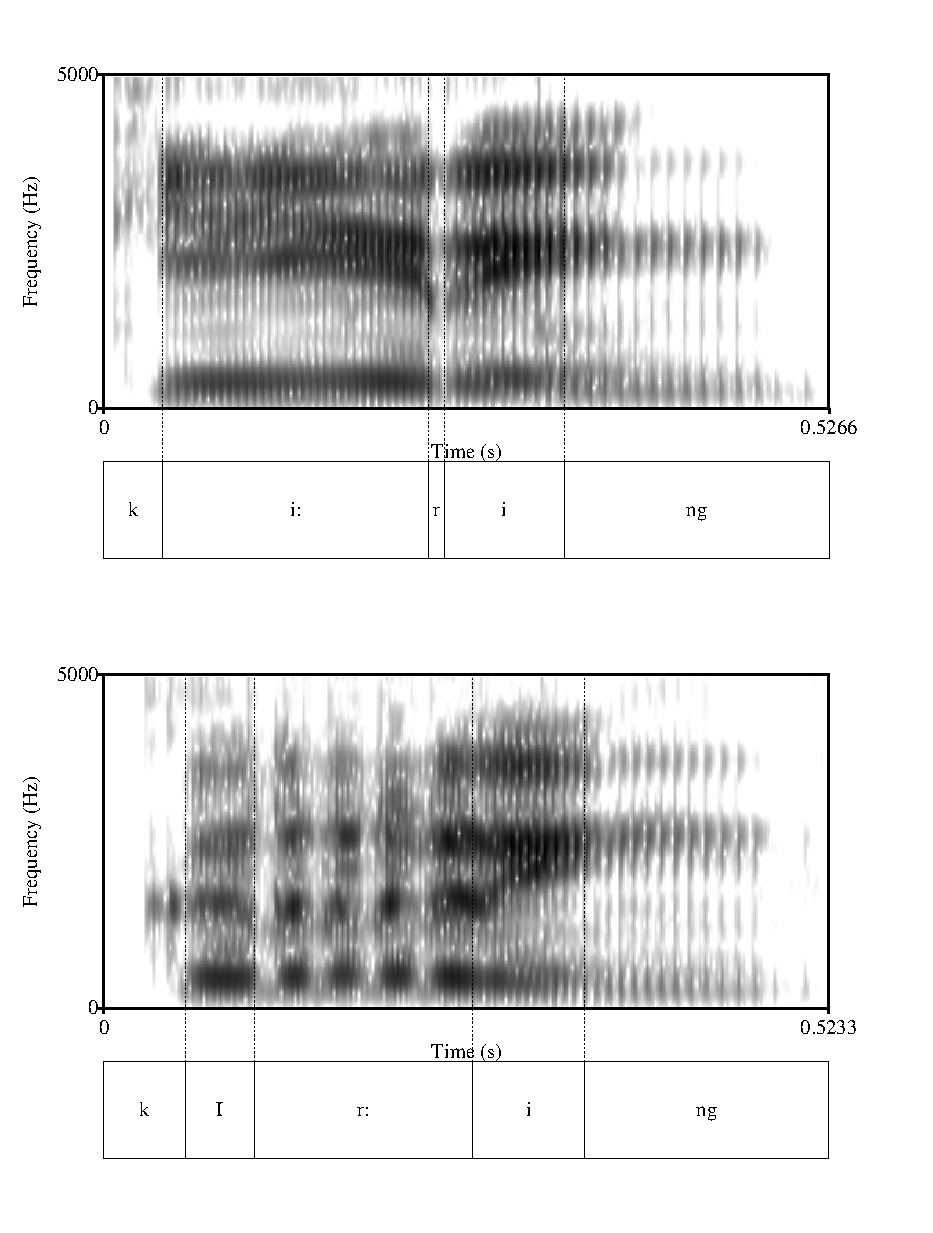
\includegraphics[width=.8\textwidth]{pics/kiiringkirring.eps}
 % pErrang-spectro.png: 432x252 pixel, 72dpi, 15.24x8.89 cm, bb=0 0 432 252
 \caption[Differences in length and vowel quality between \phontrs{ki:RiN}{send}   and \phontrs{kIr:iN}{dry}]{The words \phontrs{ki:RiN}{send} (above) and \phontrs{kIr:iN}{dry} (below) show a number of things. First, the formant structure of the first vowel is different, showing that [i] as a realization of /i/ must be distinguished from \phonet{I} as a realization of /\E/. Second, they show the complementary distribution of long vowels and long consonants. The word above has a long vowel (206ms) and a short consonant (11ms), while the word below has a short vowel (50ms) and a long consonant (158ms). The spectrograms furthermore show that short /r/ is realized as a tap with minimal duration, while phonemically long/geminated r is realized as a trill. }
 \label{fig:kiiringkirring}
\end{figure}

\subsubsection{Consonant length}\label{sec:phon:Consonantlength}

All consonants besides the prenasalized stops, \dentd{} and \V{} can occur lengthened in intervocalic position. Long vowels and long consonants are mutually exclusive. \xref{ex:phon:longcons:thiikam} shows a near minimal pair with a) a long vowel and a short consonant and b) a short vowel and a long consonant (see also Figure \ref{fig:soopithoppi}).

\xbox{14}{
\ea \label{ex:phon:longcons:thiikam}
\ea
\gll  so:pi \rm CV\textipa{:}CV \\
      liquor   \\
\ex
\gll \dentt op:i \rm CVC\textipa{:}V\\
hat\\
\z
\z
} \\

\begin{figure}
 \centering
 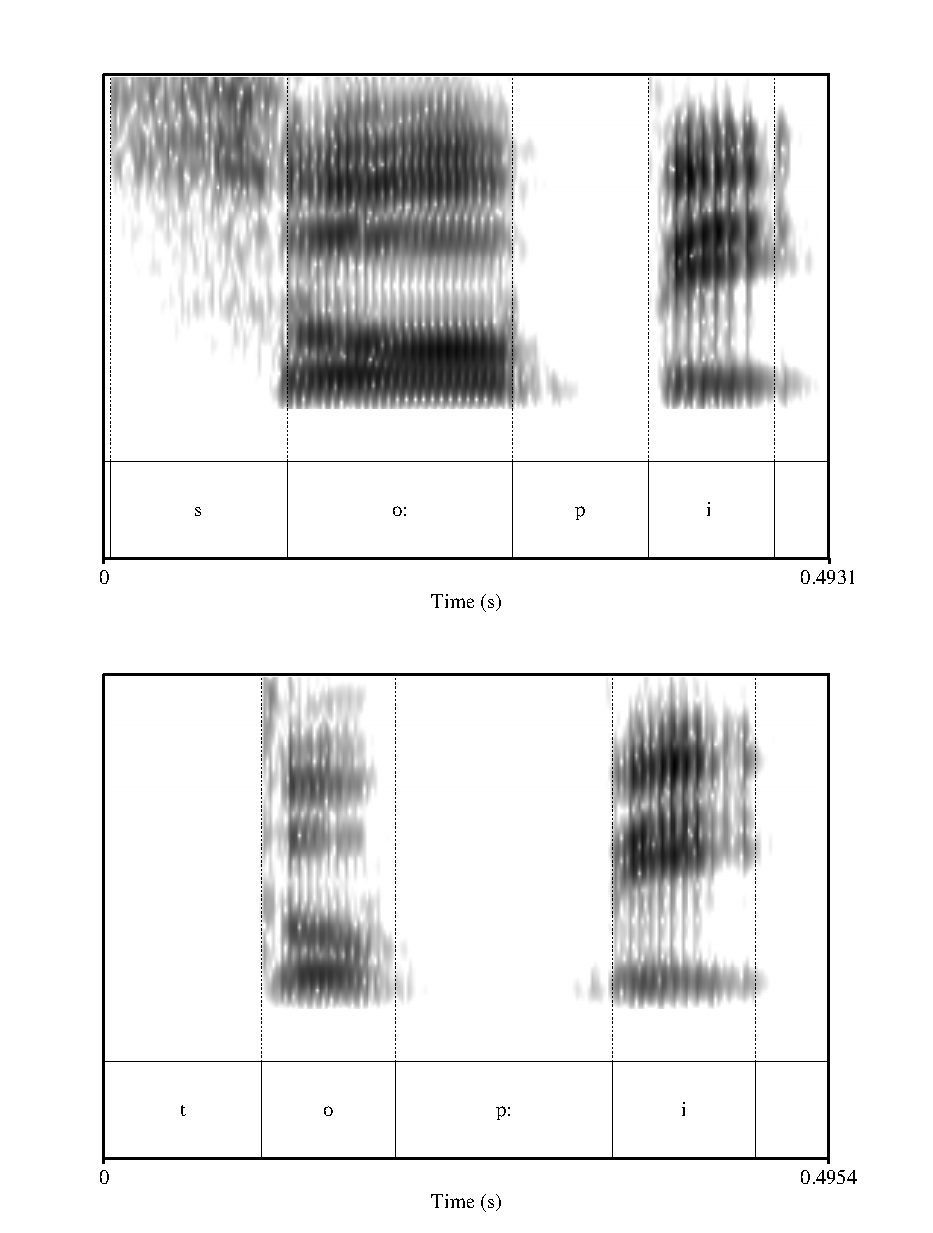
\includegraphics{pics/soopithoppi.eps}
 % soopithoppi.eps: 1179668x1179666 pixel, 0dpi, infxinf cm, bb=
 \caption[Vowel and consonant length in \phontrs{so:pi}{liquor} and \phontrs{\dentt op:i}{hat}]{The word \phontrs{so:pi}{liquor} has a long vowel (153ms) and a short consonant (93ms), while the word \phontrs{\dentt op:i}{hat} has a short vowel (91ms) and a long consonant (149ms).}
 \label{fig:soopithoppi}
\end{figure}





Two types of long consonants can be distinguished on phonological grounds: Underlyingly long consonants, as in \phontrs{\dentt op:i}{hat}{} or \phontrs{ik:a\ng}{fish}, and lengthened consonants such as in \phontrs{s\I g:aR}{healthy}. The former  always have a long consonant,\footnote{In certain types of compound, like \phontrs{kap:al+\dentt IRbaN=kapal\dentt IRbaN}{ship+fly=plane}
the long consonant optionally disappears. These are rare.} while the latter only have a long consonant if the consonant is located between penultimate and final syllable. If, through affixation, the consonant is found at another position, it is not geminated. Lengthened consonants can only occur after schwa, while underlyingly long consonants can occur after /a/ \phontrs{a\dentt:as}{top}, /e/ \phontrs{pe\dentt:a}{parrot}, /i/ \phontrs{ik:a\ng}{fish}{} and  /o/ \phontrs{\dentt op:i}{hat}. No long consonant has been found after /u/ or schwa.
Tables \ref{tab:PositionsAndGeminationsOfConsonants:stops} and \ref{tab:PositionsAndGeminationsOfConsonants:other}  contain a column of words with long consonants.

There is only one instance of a long palatal glide, \phontrs{maj:e\dentt}{corpse}.

Phonetically, long consonants are of about 1.5 times the duration of shorter consonants, as can be seen from Figure \ref{fig:soopithoppi}.

% \begin{figure}
%  \centering
%  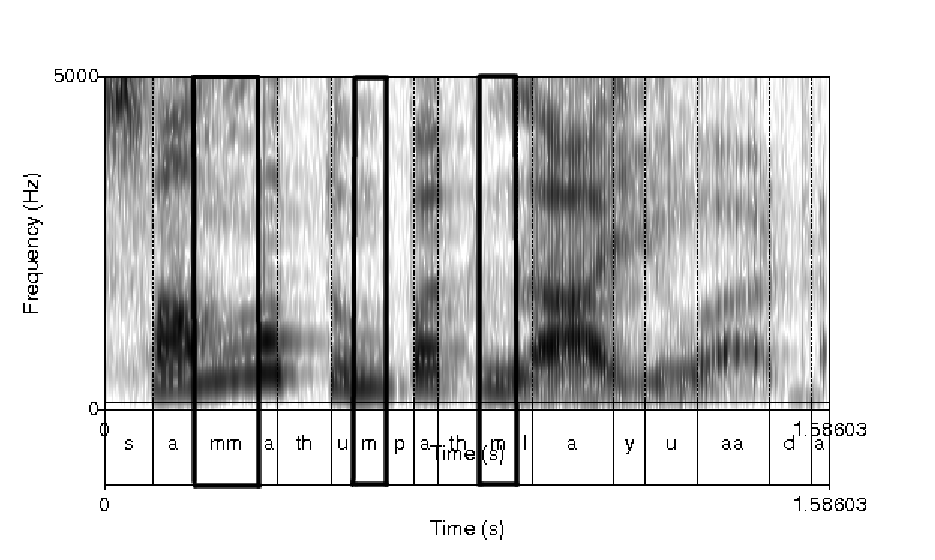
\includegraphics[height=0.3\textheight]{./pics/sammathumpathmlaayuaada.eps}
%  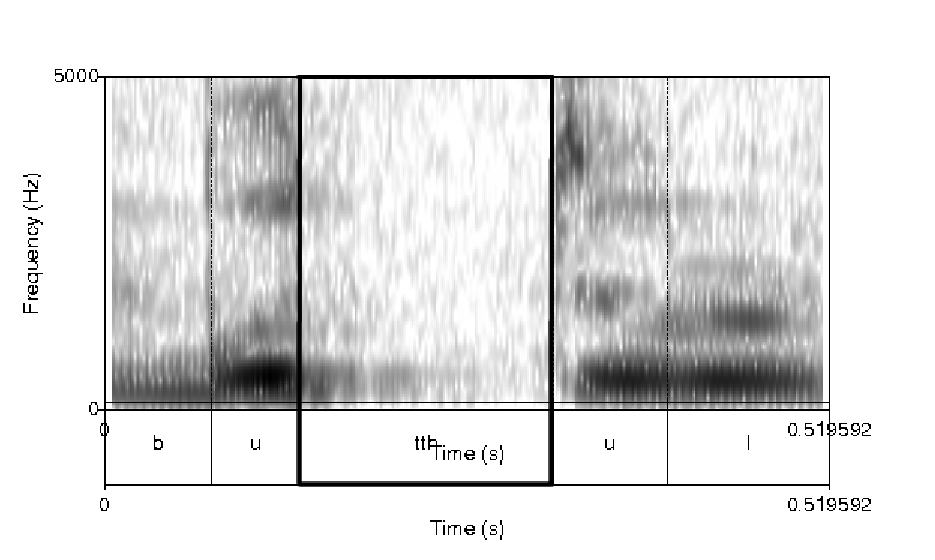
\includegraphics[height=0.3\textheight]{./pics/butthul-length.eps}
%  \caption{The first occurrence of [m] in the spectrogram above is a long consonant. Its duration is 0.144s. The further occurrences are short, the second one lasts 0.072s, the third one, 0.083s. Below, we see a long dental stop in the word \phontrs{bu\dentt:ul}{very}.}
%  \label{fig:phon:conslength:sammathumpathmlaayuaada}
% \end{figure}
% 
% \begin{figure}
%  \centering
%  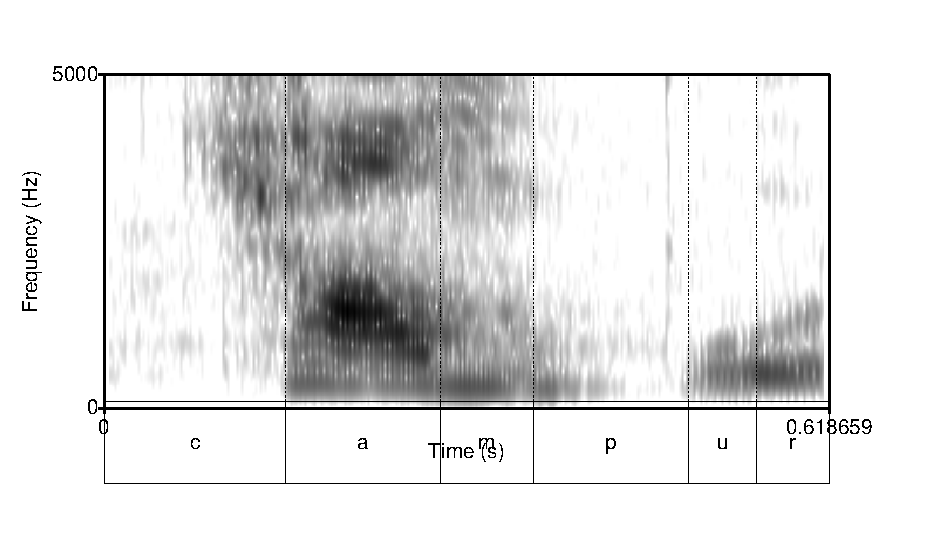
\includegraphics[height=0.3\textheight]{./pics/campur.eps}
%  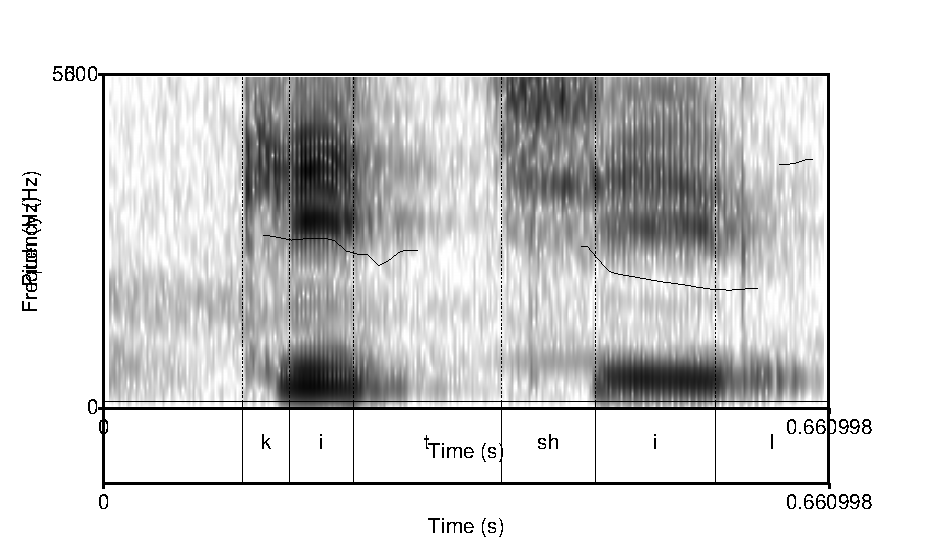
\includegraphics[height=0.3\textheight]{./pics/kiccil.eps}
% \caption{When long palatal stops are pronounced as affricates, the occlusion part last slightly longer than the fricative part. Above, we see a short palatal in the onset, while below in the word \phontrs{kic:il}{small}, the occlusion part has a duration of 0.131ms, and the fricative part has a duration of 0.082s.}
%  \label{fig:phon:conslength:kiccil}
% \end{figure}


\subsubsection{Distribution of consonants}\label{sec:phon:Distributionofconsonants}
All consonants may occur in intervocalic position, but \dentd{} is very rare there, one instance is \phontrs{kO\dentd aRa\dentt}{miracle}.
All consonants but \ng{} and the prenasalized stops may occur in  word-initial position, but the palatal glide is very rare there. There is only one word with initial \tz{}, \phonet{\tz ak:a\dentt a}, which emphasizes the rapid nature of an event and might very well be onomatopoetic, so that it would not have to obey the general phonological rules.

There are more constraints word-finally. Voiced stops, apical stops,  h, \ny{}\footnote{These four cannot occur word-finally in Sinhala, Tamil or Jakartanese either. -h\# can occur in Std. Malay, but the other three cannot.} and \V{}  cannot occur in final position in native words, although some of those are frequently found in English loan words (\em bag, pitch, bat\em).

Few consonants ever occur in the coda of syllables inside a morpheme. Those that do occur are the nasals, the liquids, /k/ and /s/ (see Tables \ref{tab:PositionsAndGeminationsOfConsonants:stops} and \ref{tab:PositionsAndGeminationsOfConsonants:other}). If roots combine with an affix or a clitic with an onset, like \phontrs{-king}{\textsc{caus}}{} or \phontrs{=pe}{\textsc{poss}}, any consonant which can occur morpheme-finally can occur in a word-medial coda.

Tables \ref{tab:PositionsAndGeminationsOfConsonants:stops} and \ref{tab:PositionsAndGeminationsOfConsonants:other} show examples for every consonant in initial and final position and also give  examples of the consonant in intervocalic position (short and long) and morpheme-internal coda position.


\begin{table}
	\begin{center}
		\begin{tabular}{llllll}
			& initial 			& intervocalic 	short		& intervocalic long & 	\parbox{2cm}{morpheme-internal coda}	 & final \\ % add column V_.CV
	\hline \vspace{0.2cm}
		p 	& \parbox[t]{2cm}{\textipa{pa:ke}\\`dress'}  & \parbox[t]{2cm}{\textipa{ba:pa}\\`father'}    & \parbox[t]{2cm}{\textipa{l\U p:as}\\`leave'} & \fbox{\parbox[t]{2cm}{~\\}} & \parbox[t]{2cm}{\textipa{g\I l:ap}\\`dark'} \\\vspace{0.2cm}
		\dentt  & \parbox[t]{2cm}{\textipa{\dentt a:na}\\`soil'}& \parbox[t]{2cm}{\textipa{u:\dentt an}\\`forest'}& \parbox[t]{2cm}{\textipa{a\dentt:as}\\`up'}      & \fbox{\parbox[t]{2cm}{~\\}} & \parbox[t]{2cm}{\textipa{bansa\dentt}\\`bedbug'} \\\vspace{0.2cm}
		t 	& \fbox{\parbox[t]{2cm}{~\\}}& \parbox[t]{2cm}{\textipa{ba:\tz ok}\\`coconut.shell'}&\fbox{\parbox[t]{2cm}{(\textipa{ka\postalvt:il})\\`bed'(Tam.)}} & \fbox{\parbox[t]{2cm}{~\\}} & \fbox{\parbox[t]{2cm}{~\\}}  \\\vspace{0.2cm}
		c	& \parbox[t]{2cm}{\textipa{campuR}\\`mix'}& \parbox[t]{2cm}{\textipa{ku:ci\ng}\\`cat'}    & \parbox[t]{2cm}{\textipa{kic:il}\\`small'}&\fbox{\parbox[t]{2cm}{~\\}}&\fbox{\parbox[t]{2cm}{~\\}}  \\\vspace{0.2cm}
		k 	& \parbox[t]{2cm}{\textipa{ka:ki}\\`leg'}    & \parbox[t]{2cm}{\textipa{ba:kaR}\\`burn'}     & \parbox[t]{2cm}{\textipa{ik:a\ng}\\`fish'} &\parbox[t]{2cm}{\textipa{\dentt aksiR}\\`think'}& \parbox[t]{2cm}{\textipa{sa:nak}\\`relatives'} \\\vspace{0.2cm}
		b 	& \parbox[t]{2cm}{\textipa{ba:pa}\\`father'} & \parbox[t]{2cm}{\textipa{Ra:ba}\\`stroke'}    & \parbox[t]{2cm}{\textipa{kb:O\ng}\\`estate'}& \fbox{\parbox[t]{2cm}{(\textipa{ib.li:s})\\`demon'(Ar.)}} & \fbox{\parbox[t]{2cm}{~\\}} \\\vspace{0.2cm}
		\dentd  & \parbox[t]{2cm}{\textipa{\dentd a:\dentt ang}\\`come'} & \fbox{\parbox[t]{2cm}{(\textipa{kO\dentd aRa\dentt})\\`miracle'(Ar.)}} & \fbox{\parbox[t]{2cm}{~\\}} & \fbox{\parbox[t]{2cm}{~\\}} & \fbox{\parbox[t]{2cm}{~\\}}  \\\vspace{0.2cm}
		d 	& \parbox[t]{2cm}{\textipa{\postalvd a:gi\ng}\\`meat'} & \parbox[t]{2cm}{\textipa{a:\dz a}\\`exist'} & \parbox[t]{2cm}{\textipa{p\U \dz:as}\\`spicy'} & \fbox{\parbox[t]{2cm}{~\\}} &\fbox{\parbox[t]{2cm}{~\\}}  \\\vspace{0.2cm}
		\J 	& \parbox[t]{2cm}{\textipa{\J a:lang }\\`walk'}& \parbox[t]{2cm}{\textipa{bla:\J aR}\\`learn'}& \parbox[t]{2cm}{\textipa{ki\J:a}\\`do'}       & \fbox{\parbox[t]{2cm}{~\\}} &\fbox{\parbox[t]{2cm}{(\textipa{ha\J})\\`Hajj' (Ar.)}}  \\\vspace{0.2cm}
		g 	& \parbox[t]{2cm}{\textipa{ga:\J a}\\`elephant'} & \parbox[t]{2cm}{\textipa{ga:gak}\\`crow'}& \parbox[t]{2cm}{\textipa{s\I g:aR}\\`healthy'}& \fbox{\parbox[t]{2cm}{~\\}} & \fbox{\parbox[t]{2cm}{~\\}} \\\vspace{0.2cm}
		\end{tabular}
		\caption[Positions and gemination of stops]{Positions and gemination of stops. Boxed fields show positions not used in native words. If an example is given, it is from a loanword.}
		\label{tab:PositionsAndGeminationsOfConsonants:stops}
	\end{center}
\end{table}


\begin{table}
	\begin{center}
		\begin{tabular}{llllll}
			& initial 			& intervocalic 	short		& intervocalic long & 	\parbox{2cm}{morpheme-internal coda}	 & final \\ % add column V_.CV
	\hline \vspace{0.2cm}
		m 	& \parbox[t]{2cm}{\textipa{ma:ka\ng}\\`eat'} & \parbox[t]{2cm}{\textipa{sa:ma}\\`together'}  & \parbox[t]{2cm}{\textipa{sam:a}\\`every'}  &\parbox[t]{2cm}{\textipa{lompa\dentt}\\`jump'}& \parbox[t]{2cm}{\textipa{ga:Ram}\\`salt'} \\\vspace{0.2cm}
		n 	& \parbox[t]{2cm}{\textipa{na:si}\\`rice'} & \parbox[t]{2cm}{\textipa{a:nak}\\`child'}       & \parbox[t]{2cm}{\textipa{b\I n:a\ng}\\`thread'}&\parbox[t]{2cm}{\textipa{ba\dentn\dentt u}\\`help'}& \parbox[t]{2cm}{\textipa{bi\dentn\dentt an}\\`star'} \\\vspace{0.2cm}
		\ny 	& \parbox[t]{2cm}{\textipa{\ny a:Ri}\\`today'} & \parbox[t]{2cm}{\textipa{m\super wo:\ny et}\\`monkey'}& \parbox[t]{2cm}{\textipa{ba\ny:ak}\\`much'}    &\parbox[t]{2cm}{\textipa{kO\ny ci}\\`key'}&     \fbox{\parbox[t]{2cm}{~\\}}  \\\vspace{0.2cm}
		\ng 	& \fbox{\parbox[t]{2cm}{~\\}} 		& \parbox[t]{2cm}{\textipa{a:\ng i\ng}\\`air'}    & \parbox[t]{2cm}{\textipa{\dentt\I\ng:a}\\`middle'} &\parbox[t]{2cm}{\textipa{ma\ng kok}\\`mug'}& \parbox[t]{2cm}{\textipa{a:ja\ng}\\`chicken'} \\\vspace{0.2cm}
		s 	& \parbox[t]{2cm}{\textipa{sa:ma}\\`with'}   & \parbox[t]{2cm}{\textipa{ka:si}\\`give'}      & \parbox[t]{2cm}{\textipa{as:am}\\`sour'}   &\parbox[t]{2cm}{\textipa{miskin}\\`poor'}& \parbox[t]{2cm}{\textipa{l\U p:as}\\`leave'} \\\vspace{0.2cm}
		h 	& \parbox[t]{2cm}{\textipa{ha:Rum}\\`bad.smell'} & \parbox[t]{2cm}{\textipa{la:heR}\\`be.born'} & \parbox[t]{2cm}{\textipa{\J ah:a\dentt}\\`wicked'} &\fbox{\parbox[t]{2cm}{~\\}}& \fbox{\parbox[t]{2cm}{~\\}}  \\\vspace{0.2cm}
		r 	& \parbox[t]{2cm}{\textipa{Ra:ba}\\`stroke'} & \parbox[t]{2cm}{\textipa{ga:Ram}\\`salt'}     & \parbox[t]{2cm}{\textipa{b\I r:as}\\`rice'}  &	\parbox[t]{2cm}{\textipa{aR\dentt iyan}\\`meaning'}& \parbox[t]{2cm}{\textipa{bla:\J aR}\\`learn'} \\\vspace{0.2cm}
		l 	& \parbox[t]{2cm}{\textipa{la:\dz a}\\`pepper'} & \parbox[t]{2cm}{\textipa{sa:la}\\`wrong'}     & \parbox[t]{2cm}{\textipa{p\U l:am}\\`slow'}  &\parbox[t]{2cm}{\textipa{salba}\\`escape'}& \parbox[t]{2cm}{\textipa{kap:al}\\`ship'} \\\vspace{0.2cm}
		\V 	& \parbox[t]{2cm}{\textipa{\V a\dentt:u}\\`time'}    & \parbox[t]{2cm}{\textipa{ka:\V i\ng}\\`marry'}& \fbox{\parbox[t]{2cm}{~\\}}&\fbox{\parbox[t]{2cm}{~\\}}& \fbox{\parbox[t]{2cm}{~\\}} \\\vspace{0.2cm}
		j 	& \fbox{\parbox[t]{2cm}{(\textipa{ja\dentt i:m})\\`orphan'(Ar.)}}    & \parbox[t]{2cm}{\textipa{sa:ja\ng}\\`love'}& \parbox[t]{2cm}{\textipa{maj:e\dentt}\\`corpse'}&\fbox{\parbox[t]{2cm}{~\\}}& \parbox[t]{2cm}{\textipa{bukulaj}\\`fight'} \\\vspace{0.2cm}
		\end{tabular}
		\caption[Positions and gemination of other consonants]{Positions and gemination of other consonants. Boxed fields show positions not used in native words. If an example is given, it is from a loanword.}
		\label{tab:PositionsAndGeminationsOfConsonants:other}
	\end{center}
\end{table}
 

\subsection{Do the glides pattern with vowels or with consonants?}\label{sec:phon:Dotheglidespatternwithvowelsorwithconsonants}
The labiodental approximant \V{} and the palatal approximant j are treated as phonological consonants in this grammar. Given that the approximants are on an intermediate position between consonants and vowels, it would equally be possible to treat them as vowels.\footnote{\citet[116]{Himmelmann2005typochar} reports that this problem is common in Austronesian languages and that, in most cases, the `consonantal' analysis can be shown to be superior.} This fails to capture some important facts. First, tautosyllabic sequences VG,\footnote{Excluding geminates like in \phontrs{maj:e\dentt}{corpse}.} where G is one of the two approximants, only occur word-finally, like in \phontrs{bukulaj}{fight}. Sequences of VG do not occur before a consonant.  Treating the approximants as vowels would lead to the postulation of complex nuclei VV only for final syllables, whereas treating them as consonants avoids this and is in line with general syllable structure in SLM, which permits the structure VC (Section \ref{sec:phon:Syllablestructure}).

Complex nuclei could be postulated for words like \phontrs{bja:sa}{habit} or \phontrs{p\V a:sa}{fasting period}, but this is not necessary either, since complex onsets are needed in this position anyway, illustrated by examples like \phontrs{bla:\J aR}{learn}{} or \phontrs{cRi:\dentt a}{story}.

Analyzing these approximants as vowels would needlessly complicate syllable structure, while analyzing them as consonants is fine with overall syllable structure, which permits final codas and complex onsets for the problematic positions where the approximants meet a vowel.%\footnote{Also see \citet{Clynes1997} for similar argumentation for Proto-Austronesian. While Proto-Austronesian is of course of a completely different period, the arguments for the phonological status of the glides are comparable.}


% cokke sokku
% cakke sakku waste of tea, meat,
% cavulang savulan crazy dancing

\section{Suprasegmentals}\label{sec:phon:Suprasegmentals}
The only suprasegmental which seems to of (albeit limited) relevance for SLM is vowel harmony. Vowel harmony might have or have had an influence on the realization  of raised schwa as a front or back high vowel (see Section \ref{sec:phon:allophonesofschwa:frontingandretracting}).

The following suprasegmental features have not been found to be relevant for SLM phonology: \em stress, tone, \em and \em nasal harmony\em.
Nasal harmony is not present in many languages and its absence will not be discussed here.
While tone is more common in the world's languages, its absence in SLM is not surprising either, given that neither the ancestor varieties nor the adstrates have lexical tone. Tone will not be discussed any further either, but see Section \ref{sec:phon:Intonation} for intonation patterns.
 A more intriguing feature is the absence of stress, which cannot be determined phonetically or phonologically. There are no cues of pitch or intensity, and vowel quality is inconclusive as well. This will be discussed in more detail in Section \ref{sec:phon:SLMasastresslesslanguage}, after having established the general properties of the syllable.


\section{Syllable structure}\label{sec:phon:Syllablestructure}
SLM syllables may have a complex onset and a simple coda. Both onset and coda are optional.  Word-initially,  /s-/ may precede nost of the consonants. Long vowels and a coda may not co-occur. The general syllable structure is then

\ea (s)(C)(L)V(X)\z

where L is either /l,r,\V,j/ and X is either a consonant or the additional length of the vowel.

The following examples show
\begin{itemize}
 \item   presence and absence of the onset \xref{ex:phon:sylstr:onset},
 \item   presence of a complex onset \xref{ex:phon:sylstr:complonset},
 \item   presence of initial /s-/ with simple and complex onset \xref{ex:phon:sylstr:skr},
 \item   presence and absence of the coda \xref{ex:phon:sylstr:onset},   and
 \item   mutual exclusion of long vowel and coda consonant \xref{ex:phon:sylstr:VVCC}.
\end{itemize}


\xbox{6}{
\ea \label{ex:phon:sylstr:onset}
\gll a:bu --- ca:bu\dentt \\
     ash --- remove  \\
\z
}
\xbox{6}{
\ea \label{ex:phon:sylstr:complonset}
\gll ci:\dentt ak --- cRi:\dentt a \\
     draw --- story\\
\z
}

\xbox{6}{
\ea \label{ex:phon:sylstr:skr}
\gll kRi:\ng a\dentt{} ---  skRi:\ng a\dentt\\
sweat --- having.sweat\\
\z
}
\xbox{6}{
\ea \label{ex:phon:sylstr:VVCC}
\gll so:pi --- \dentt op:i (\dentt op.pi) \\
     liquor --- hat \\
\z
}


Let us now turn to more detailed discussion of onset, nucleus and coda.

\subsection{Onset}\label{sec:phon:Onset}
There are close to no restrictions on the occurrence of individual consonants in simple onsets of syllables. Any consonant or glide may occur in the onset of a syllable (cf. Tables \ref{tab:PositionsAndGeminationsOfConsonants:stops} and \ref{tab:PositionsAndGeminationsOfConsonants:other}), but \phonem{N}{} may not occur in the absolute onset of a word.
Word internally, /\ng/ is permitted in the onset, as \phontrs{a:.\ng i\ng}{air} shows.

Complex onsets are mainly found morpheme-initially. Exceptions I am aware of are instances of \E{} dropped between b and a liquid, like \phontrs{sub(\E)la}{side} or \phontrs{lab(\E)Rak}{whack}. It is unclear as of now whether the b in these words is at the coda of the first syllable, at the onset of the last syllable, or whether these words are underlyingly still trisyllables. Other exceptions are  \phontrs{pu\dentt Ri}{queen} and \phontrs{kOmplOk}{bush}.

Complex onsets are limited to  combinations of stop or s combined with liquids or glides,  and m+l and m+j, as shown in Table \ref{tab:ComplexOnsets}. Apical stops are not found in complex onsets, with the exception of \phontrs{=\dz(\E{})\rz i\ng}{\textsc{abl}} and \phontrs{=\postalvd(e)\rz ampa\dz a}{they}.\footnote{It is unclear why the rhotic is retroflex in the former case and postalveolar in the latter.} It is interesting to note that while all coronal voiced stops in native words are apical in intervocalic position, dental articulation can also be found in initial position, as shown by the pair \phontrs{\dz u:\V a}{two} and \phontrs{\dentd u:a}{prayers}. Apical articulation is still more common overall, but if a liquid follows, dental articulation is the norm, as in \phontrs{\dentd la:pan}{eight}, \phontrs{\dentd Ra:pa}{how much?}, and  \phontrs{\dentd Ra:ka}{hell}.

Complex onsets starting with /m-/ are also found. There are a number of /ml-/ onsets, but no /mr-/ onsets. Some informants claim that there is an onset /m\ny/ in \phontrs{m\ny a:lak}{catch fire}, but it was found that this word is is normally pronounced as \phonet{mja:lak}.

\begin{table}
	\begin{center}
	% use packages: array
		\begin{tabular}{lllll}
			& ~~~~~r 			& ~~~~~l & ~~~~~\V & ~~~~~j\\
\hline
		p 	& \phontrs{pRompa\ng}{girl}   & \phontrs{pli:\dentt a}{lamp}&\phontrs{p\V a:sa}{fasting}&\phontrs{pja:Ra}{adopt}\\
		\dentt  & \phontrs{\dentt Ra:}{\textsc{neg}}   		& \phontrs{\dentt la:\nJ a\ng}{naked}&&\\
		t	&    & &&\\
		c	& \phontrs{cRi:\dentt a}{story}   & \phontrs{cla:na}{trousers}&&\\
		k 	& \phontrs{kRe:\dentt a}{cart}   	& \phontrs{kla:pa}{coconut}&\phontrs{k\V a:li}{pot}&\\
		b 	& \phontrs{bRa:nak}{birth}   & \phontrs{bla:ka\ng}{after}&\phontrs{b\V a:ja}{crocodile}&\phontrs{bja:sa}{habit}\\
		\dentd  & \phontrs{\dentd Ra:pa}{how.many}& \phontrs{\dentd la:pan}{eight}&&\\
		d 	& (\phontrs{\dz(e)\rz ampa\dz a}{they})  	& &&\\
		\J 	& \phontrs{\J Ra:\V a\dentt}{pimple}\footnotemark   & \phontrs{\J le:na}{window}&&\\
		g 	& \phontrs{gRe:\J a}{church}  & \phontrs{glu:\dz up}{thunder}&&\\
		s   	& \phontrs{sRa:\dentt us}{one.hundred}  & \phontrs{slampe}{handkerchief}&\phontrs{s\V a:Ra}{noise}&\phontrs{sja:nu}{this person} \\
		m   	&     	& \phontrs{mla:Ra\dentt }{difficult}&&\phontrs{mja:lak}{catch fire}\\
		\end{tabular}
		\caption{Complex onsets}
		\label{tab:ComplexOnsets}
	\end{center}
 \end{table} 
\footnotetext{I would like to thank Uri Tadmor for suggesting this word.}

\citet{Bichsel} states that syllables may not start with a vowel and that a preposed glottal stop is used to prevent this. This analysis is shared by \citet{Tapovanaye1995}. My data do not support this  (See Section \ref{sec:phon:Consonants}).



\subsection{Nucleus}\label{sec:phon:Nucleus}
The nucleus normally consists of one vowel, which is long in open penultimate syllables of disyllables and trisyllables with initial schwa. Some words could be seen as having a rising diphthong \phontrs{bja:sa}{habit}, \phontrs{s\V a:Ra}{sound}, but these are analyzed as complex onsets here.

Nasals left over after schwa deletion become syllabic, such as \phonem{@mpa\dentt}`four', realized as \phonet{Umpa\dentt} or \phonet{\s{m}pa\dentt} after deletion of schwa (see Section \ref{sec:phon:schwa:deletion}).

\subsection{Coda}\label{sec:phon:Coda}
Syllables may have a simple coda. Morpheme-medially, the coda is most often identical to the following onset (\phontrs{ik.ka\ng}{fish}), or a homorganic nasal (\phontrs{ba\dentn\dentt u}{help}), but /s, l, r, k/ are also found (\phontrs{mis.kin}{poor}, \phontrs{kal.\dentt Ra}{unless},  \phontrs{kaR.cel}{problem}, \phontrs{\dentt ak.siR}{think}). The velar nasal \phonem{N} is also found before /s/, as in \phontrs{baNsa}{ethnic group}, alongside the expected homorganic nasal found for instance in \phontrs{bansa\dentt}{bedbug}. Apical or palatal stops are never found in the coda, neither are voiced stops or /h/. Morpheme-finally, /p/ and /\dentt{}/ are allowed in addition to the consonants named above, but /\ny{}/ is impossible. Examples of coda position for the remaining consonants can be found in Tables \ref{tab:PositionsAndGeminationsOfConsonants:stops} and \ref{tab:PositionsAndGeminationsOfConsonants:other} on page \pageref{tab:PositionsAndGeminationsOfConsonants:stops}.

Given that voiced consonants never occur in coda position, the theoretical problem arises whether the coda stops are phonologically always voiceless, or whether some might be phonologically voiced and undergo final devoicing. The nominalizer \em -an \em can be used to test this because it has no onset. The root-final coda consonant is then resyllabified and found in onset position, where final devoicing is ruled out. It turns out that all coda consonants remain voiceless in this position, which shows that the lack of voicing is present in the underlying form and not caused by final devoicing. An example would be \phontrs{\dentt u:\dentt up}{close} and \phontrs{\dentt u\dentt u\{p/*b\}an}{closing}.



\subsection{Initial /s-/}\label{sec:phon:Initials}
The phoneme /s/ can be found preceding an onset consonant. Sometimes this can be analyzed as reduction of the nucleus as in \phonet{s(@).la:.ma\dentt}, `greetings' or \phonet{(a)s.ma:.ka\ng} `having eaten'. In these cases, the non-reduced form also exists. In other cases however, the non-reduced form does not exist. Cases in point are  \phontrs{spa:Ru}{some}{} and \phontrs{sbi:lan}{nine}. Table \ref{tab:SClusters} gives an overview of the possibilities.

\begin{table}
	\centering
		\begin{tabular}{rcccccc}
					& labial     		& dental 			& apical 		& palatal   	& velar \\
			\hline
			voiceless stop	&\tbltrs{spa:Ru}{some}	&\tbltrs{s\dentt\I\ng\textipa{:}a}{half}	&n/a	&\tbltrs{(scu:ci)}{\textsc{cp}-wash}	&\tbltrs{ska:Ra\ng}{now}\\ \\
			voiced stop	&\tbltrs{sbi:lan}{nine}	& \tbltrs{(s\dentd a:\dentt aN)}{\textsc{cp}-come}	 &\tbltrs{s\postalvd i:ki\dentt}{few}&\tbltrs{(s\J a:la\ng)}{\textsc{cp}-walk}	& \tbltrs{(sga:li)}{\textsc{cp}-dig}\\\\
			nasal		&\tbltrs{(sma:\dentt i)}{\textsc{cp}-dead}& 	n/a	&\tbltrs{sna:pan}{gun}	&\tbltrs{(s\ny a:\ny i)}{\textsc{cp}-sing}&n/a\\\\
			lateral		&	n/a		&	n/a			& \tbltrs{sla:lu}{sad}	& n/a 			& n/a \\\\
			rhotic		&	n/a		&	n/a			&\tbltrs{sRi:bu}{1,000} & n/a 			& n/a \\\\
			approximant 	&\tbltrs{s\V a:Ra}{sound}& 	n/a			& n/a			&\tbltrs{sja:nu}{this.person}	& n/a \\\\
		\end{tabular}
	\caption[S-clusters]{S-clusters. S-clusters are possible in many combinations. These are indicated here. S-clusters cannot be formed with fricatives in SLM. Phonemes which are either not found at all in SLM, or not found in initial position, cannot form S-clusters. This is indicated by n/a. Some S-clusters could not be found in monomorphemic words, but only in combination with the conjunctive participle prefix \phonet{(a)s(\E)-}.  These are indicated by parentheses.\\ }
	\label{tab:SClusters}
\end{table}

In line with general findings about the syllabification of elements which do not show lower sonority than the element they precede, /s-/ before stops would be extrasyllabic \citep{HalleEtAl1980,Wiese1988}, and would form a complex onset before sonorants, according to the Core Syllabification Principle \citep[299]{Clements1990sonority}. %\footnote{Before  stops, /s-/ is extrasyllabic, while it forms complex onsets before sonorants (but see \citet{FarrisTrimble2007alt} for an argument that other S-clusters might be extrasyllabic as well).} 
A representation of extrasyllabic /s-/ is given in \xref{ex:phon:s:sbanthu} for \phontrs{sba\dentn\dentt u}{having helped}, while a representation for the complex onset is given in \xref{ex:phon:s:slampe} for \phontrs{slampe}{handkerchief}.\footnote{Unnecessary detail is removed from these representations. More detailed representations can be found below.}


\xbox{7}{ 
\ea\label{ex:phon:s:sbanthu}
\begin{tabular}{cc}
\multicolumn{2}{c}{~~$\omega$}\\\\\\
~~~~~~ $\sigma$\begin{picture}(0,0)\put(0,10){\line(1,6){5}}  \end{picture}  &$\sigma$\begin{picture}(0,0)\put(-8,10){\line(-1,2){15}}\end{picture}\vspace{0,3cm} \\
~~~~~~O\begin{picture}(0,0)\put(-2,10){\line(1,1){10}}\end{picture}
N\begin{picture}(0,0)\put(-2,10){\line(0,5){10}}\end{picture}
C\begin{picture}(0,0)\put(-2,10){\line(-1,1){10}}\end{picture}
&
O\begin{picture}(0,0)\put(-2,10){\line(1,2){5}}\end{picture}
~N\begin{picture}(0,0)\put(-2,10){\line(-1,2){5}}\end{picture}\\
\\
s\begin{picture}(0,0)\put(0,10){\line(2,5){33}}\end{picture}
~~~~b\begin{picture}(0,0)\put(-2,10){\line(0,5){10}}\end{picture}
~a\begin{picture}(0,0)\put(-2,10){\line(0,5){10}}\end{picture}
~n\begin{picture}(0,0)\put(-2,10){\line(0,5){10}}\end{picture}
&
\dentt\begin{picture}(0,0)\put(-2,10){\line(0,5){10}}\end{picture}
~u\begin{picture}(0,0)\put(-2,10){\line(0,5){10}}\end{picture}\\
\end{tabular}
\z
}
\xbox{7}{
\ea\label{ex:phon:s:slampe}
\begin{tabular}{cc}
\multicolumn{2}{c}{~~~~$\omega$}\\\\\\
~~$\sigma$\begin{picture}(0,0)\put(-3,10){\line(1,2){14}}  \end{picture}  &$\sigma$\begin{picture}(0,0)\put(-5,10){\line(-1,2){14}}\end{picture}\vspace{0,3cm} \\
O\begin{picture}(0,0)\put(-2,10){\line(1,1){10}}\end{picture}
~N\begin{picture}(0,0)\put(-2,10){\line(0,5){10}}\end{picture}
~~~C\begin{picture}(0,0)\put(-2,10){\line(-1,1){10}}\end{picture}
&
O\begin{picture}(0,0)\put(-2,10){\line(1,2){5}}\end{picture}
~~~N\begin{picture}(0,0)\put(-4,10){\line(-1,2){5}}\end{picture}\\\\
s\begin{picture}(0,0)\put(-2,10){\line(1,5){3}}\end{picture}
~l\begin{picture}(0,0)\put(-2,10){\line(-1,5){3}}\end{picture}
~a\begin{picture}(0,0)\put(-2,10){\line(0,5){10}}\end{picture}
~~~m\begin{picture}(0,0)\put(-4,10){\line(0,5){10}}\end{picture}
&
p\begin{picture}(0,0)\put(-4,10){\line(0,5){10}}\end{picture}
~~~e\begin{picture}(0,0)\put(-2,10){\line(0,5){10}}\end{picture}\\
\end{tabular}
\z
} \\






% Given that final consonants are often aspirated, and final vowels can receive a glottal stop, final word boundaries can be speculated to be marked by a feature [+glottal], which is not found elsewhere in SLM phonology (with the exception of /h/, which is a rare phoneme).


% \subsection{Hiatus resolution}\label{sec:phon:Hiatusresolution}
% A glide can be inserted between two vowels  to avoid hiatus, as in /\dentt uan/$\to$\phonet{\dentt u:an\~{}\dentt u\V an}. Occasionally, /h/ is also used for hiatus resolution (\phonet{\dentt u(:)han}) by certain speakers, but this is frowned upon by others. /h/ is acceptable between two identical vowels, as in \phontrs{/sala-an/}{wrong-\textsc{nmlzr}}$\to$\phonet{salahan}. \citet{Tapovanaye1995} also argues that \phontrs{poho\ng}{tree} is underlyingly /poo\ng/ with the /h/ inserted to split up the long vowel. This analysis intends to capture the fact that sequences V$_i$hV$_i$ (\phontrs{leheR}{neck})  are somehow special in that they never lengthen the first vowel, whereas sequences V$_i$hV$_j$ could do so (\phontrs{la:heR}{be.born}). The elimination of /h/ from the underlying form is however not very elegant and not  historically plausible, either. A constraint banning lengthening of vowels in V$_i$hV$_i$ environments would do the same job without distorting the phonological representation.

\section{The internal structure of the word}\label{sec:phon:Theinternalstructureoftheword}
Phonological words have an internal structure, which is based on feet, syllables and moras in SLM.\footnote{This section would never have been as detailed as it is without the help of Diana Apoussidou, for which I am extremely grateful. Most of the theoretical insights presented here are hers. All misrepresentations are my own responsibility.}
 Furthermore, the structure of the morphological word has an influence on the structure of the phonological word.
On the  morphological level, we distinguish between roots, stems and words. Roots consist of one lexeme and no additional material, stems consists of one or more lexemes plus optional additional derivational morphemes, while the word consists of a stem and inflectional material. This is illustrated in \xref{ex:phon:rootsstemswords}. Outside of the domain of the word, there can be clitics attached, which do not form part of the word proper, but are interesting for delimiting purposes. This morphological structure of the word can thus be represented as follows:

\ea\label{ex:phon:rootsstemswords}
(CLT)
	\fbox{
		(INFL)
 		\fbox{
			\fbox{LEXEME}$_{\textsc{root}}$
			(LEXEME)
			(\textsc{DERIV})
 		}$_{\textsc{stem}}$		
		(INFL)
	}$_{\textsc{word}}$
	(CLT)
\z

Generally speaking, the difference between roots and stems is not very important in SLM. Both are normally parsed into one phonological word. Material outside of the stem, like inflectional affixes and clitics, is not parsed into a phonological word with the stem.

\subsection{Roots}\label{sec:phon:struct:Roots}
Sri Lanka Malay has roots consisting of two and three syllables, plus a handful of monosyllables. The polysyllables come in  different types, listed in \xref{list:phon:wordtypes} (We disregard the difference between simple and complex onsets for this list). In the column for syllable structure, \E{} represents a phonemic schwa, which can be realized as \phonet{@,I,U,i,u} phonetically. We can distinguish 5 groups: monosyllables, disyllables without schwa, disyllables with schwa, problematic disyllables, and trisyllables. At the syllable break, we can distinguish a short consonant (V.C), a long consonant (C$_i$.C$_i$V), and a heterosyllabic cluster (C$_i$.C$_j$V).


\newcounter{mycounter}
\setcounter{mycounter}{1}

\ea\label{list:phon:wordtypes}
\begin{tabular}{@{\arabic{mycounter})\stepcounter{mycounter}~~~~~}ll@{~~~e.g.~~~}l}
& CV\textipa{:}			 & \phontrs{pi:}{go}, \phontrs{\dentt e:}{tea}, \phontrs{ca:}{tea}, \phontrs{ba:}{bring}\\
&  CVC			 & \phontrs{pon}{bride}\phontrs{\dentt aj}{excrement}\vspace{0.2cm}\\

&  (C)V.CV		 & \phontrs{ka\dentt a}{\textsc{quot}}, \phontrs{ini}{\textsc{dist}}, only found in function words\\
&  (C)V\textipa{:}.CV(C)		 & \phontrs{\dentt i:ga}{three}, \phontrs{u:\dentt a\ng}{forest}\\
&  (C)VC$_i$.C$_j$V(C)	 & \phontrs{kumpul}{collect}, \phontrs{o\dentn\dentt a}{camel}\\
&  (C)VC$_i$.C$_i$V(C)	 & \phontrs{\dentt op:i}{hat}, \phontrs{a\dentt:as}{top}\vspace{0.2cm}\\

&  C\E C$_i$.C$_j$V	& \phontrs{m\I \dentn\dentt a}{vomit}\\
&  (C)\E C$_j$.C$_j$V(C)	 & \phontrs{s\I g:aR}{healthy}, \phontrs{\dentt IN:a}{middle}\\
&  (\E)N.CVC		 & \phontrs{(\U)mpa\dentt}{four}\\
&  (\E)C$_i$.C$_i$V(C)	 & \phontrs{(\U)m:a}{mother}, \phontrs{(\I)n:am}{six}\vspace{0.2cm}\\

&  CV$_i$.h$_i$C	 & \phontrs{poho\ng}{tree}\\
&  CV.GVC		& \phontrs{lija\dentt}{see}, \phontrs{\dentt u\V an}{gentleman}\\
&  CV\textipa{:}.GVC	 & \phontrs{\dentt u:\V a}{old}, \phontrs{\J u:\V al}{sell}\vspace{0.2cm}\\

&  CV.CV.CV(C)		 & \phontrs{ku\dentt umu\ng}{see}, \phontrs{nigiRi}{country}\\
&  C\E.CV\textipa{:}.CV(C)		 & \phontrs{m\E\dz e:Ra}{flag}, \phontrs{c\E ca:\V ak}{wash}\\
&  CVC.CVC.CVC		 & \phontrs{kak:aRla\dentt}{cockroach} (only example)\\
\end{tabular}
\z

The following generalizations emerge from this list:
\begin{itemize}
 \item there is maximum of one long vowel per word
 \item long vowels are always found in the penultimate, with the exception of a few monosyllabic words
\item /\E/ in penultimate syllables is never realized as \phonet{@}, but always raised
\item no allophone of /\E/ is ever long
\item penultimate syllables with /\E/ are always closed
 \item long vowels never occur in closed syllables
 \item penultimate syllables of disyllabic words are always heavy ((C)VC or (C)V:) with the exception of function words and words with a glide or h as onset of the final syllable
 \item long vowels are never preceded by a syllable with \phonet{a,e,o}.
\end{itemize}

These generalizations point to an important role of the weight of the penultimate syllable. An analysis of these generalizations will be given in Section \ref{sec:phon:Analysisofwordstructure}.

\subsection{Stems}\label{sec:phon:struct:Stems}
Derivational suffixes like the nominalizer \em -an \em add to the size of a root. A disyllabic word can become trisyllabic through suffixation. The resulting trisyllable conforms to the same word types listed above in \xref{list:phon:wordtypes} for roots.
An example of this is \phontrs{ba:las}{answer(V)}+\phontrs{-an}{\textsc{nmlzr}}=\phontrs{balasan}{answer(N)}{} with a short vowel (Figure \ref{fig:baalasbalasan}). \phonet{*bala:san} or \phonet{*ba:lasan} are not structures listed in \xref{list:phon:wordtypes}, and are disallowed.

\begin{figure}
 \centering
 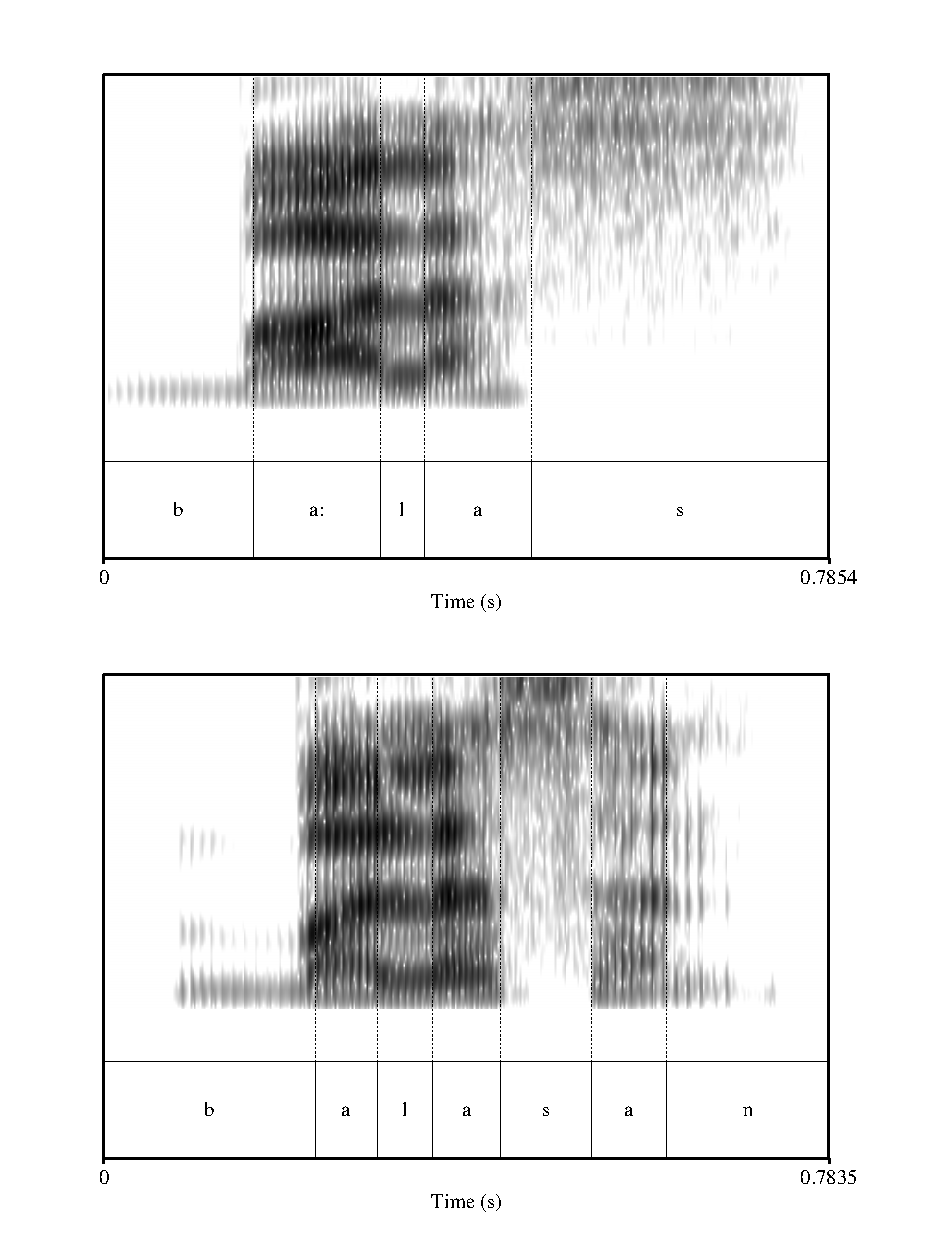
\includegraphics{pics/baalasbalasan.eps}
 % baalasbalasan.eps: 1310738x1179666 pixel, 0dpi, infxinf cm, bb=
 \caption[Absence of vowel lengthening after derivation]{The word \phontrs{ba:las}{answer(v)} has a long first vowel (138ms). This same vowel is realized as short (67ms) upon the addition of the nominalizing suffix \em -an \em.}
 \label{fig:baalasbalasan}
\end{figure}



There is one additional structure for stems which is never found in roots, namely

\begin{itemize}
 \item C\E.CV.CVC e.g. \phontrs{sIgaR-an}{healthy'+`\textsc{nmlzr}'=`health}, where the schwa is always realized as \phonet{I}.
\end{itemize}

This structure has no long vowel, but a raised schwa in the first syllable. This stem structure contrasts with the structure of trisyllabic roots, where a schwa in the initial syllable  triggers a long vowel in the penultimate. Additionally, schwa in trisyllabic roots is always realized as \phonet{@}, while here it is never realized as \phonet{\E}, but always as \phonet{I}.




The second category-changing suffix next to the nominalizer \em -an \em mentioned above is the causativizer \em -ki\ng\em, which can behave like \em -an \em in making a word trisyllabic, resulting in a short vowel. The behaviour of \em -ki\ng{} \em is a bit more complex though and is treated in more detail on page \pageref{page:phon:king}.

Similar behaviour is found for the numeral derivational suffixes \phontrs{-blas}{-teen} and \phontrs{-pulu}{-ty}, which disallow long vowels.

The   derivational prefixes, \phontrs{ka-}{\textsc{ord}} and \phontrs{k@n@-}{\textsc{invol}}, do not have any influence on the vowel length of their host.

Compound stems like \phontrs{kaca ma:\dentt a}{mirror+eye=spectacles} can only have long vowels in the last part of the compound. This is true for nominal compounds like \phonet{kaca ma:\dentt a}, but also for verbal compounds like \phontrs{kasi ka:\V i\ng}{give+marry=marry off}.


% \xbox{14}{
% \ea \label{ex:form:modals:mau:recipe}
% \gll manis-an=nang mà-thaaro guula \textbf{maau} gula paasir konnyong \textbf{maau} \\
%  sweet-\textsc{nmlzr}=\textsc{dat} \textsc{inf}-put sugar want sugar sand few want\\
% `In order to make it sweet, you need sugar, you need a bit of crystal sugar.' (B060115rcp02)
% \z
% }


\subsection{Words}\label{sec:phon:struct:Words}
The structure of stems is not changed by adding additional material on the word level, such as inflectional affixes or clitics. For instance, the quantity of the vowels remains the same if a clitic like \phontrs{=pe}{\textsc{poss}} is attached to the stem, e.g. \phontrs{ba:pa}{father}, \phontrs{ba:pa=pe}{father's} with a long vowel in both, or \phontrs{makanan=pe}{of the food}, with a short vowel as in \phonet{makanan}\#. An inflectional suffix like the imperative \em -la \em would   not change the vowel quantity of the stem it attaches to, either.

\subsection{Word length}\label{sec:phon:Wordlength}
Disyllabic roots are most common (ca. 90\%), while trisyllabic roots are more rare (ca. 10\%). Only a handful of lexical roots consists of one syllable: \phontrs{pii}{go}, \phontrs{pon}{bride}, \phontrs{\dentt e:}{tea},  and \phontrs{ca:}{tea}, besides the function words \phontrs{se:}{1s.polite}, \phontrs{go:}{1s}{familiar}, \phontrs{lu:}{2s.familiar},  and \phontrs{de:}{3s.familiar}. More than three syllables are found in the words  \phontrs{kenija:ja}{in vain} and \phontrs{bukaRijOk}{cock-a-doodle-do}. %demikian

By affixation and compounding, longer words can be formed, but more than five syllables are rarely found. The longest \em bona fide \em word (i.e. without clitics) found up to now is \phontrs{k@-sbilan-pulu}{nintieth}. If clitics are included, there is technically no longest word because clitics can be stacked infinitely (see Section \ref{sec:morph:Boundwords}, p. \pageref{sec:morph:Boundwords}).



\subsection{Syllable prominence}\label{sec:phon:Syllableprominence}
Sri Lanka Malay words do not show different levels of prominence in their syllables, neither phonologically nor phonetically. In other words, there is no word accent or stress. \citet{SmithEtAl2004} claim that ``stress falls on the long vowel of a word, or on the initial syllable if the word only contains only short vowels.'' They do not state by which acoustic cue they established the location of stress, so that we are probably dealing with an impressionistic statement here. \citet{Bakker2006} reports accent on the first syllable, drawing on \citet{Robuchon2003}. These statements again seem to be impressionistic. Some instrumental analyses were undertaken to check these claims, but no cues for a saliently prominent (stressed) syllable could be found. 49 words with different syllable structures were checked in 6 different controlled environments with two male native speakers of SLM for pitch contour and intensity. The compiled measurements taken together do not suggest that a meaningful generalization about the correlation between word structure and  pitch or intensity can be made  \citep{ApoussidouEtAl2008}.

\begin{figure}
 \centering
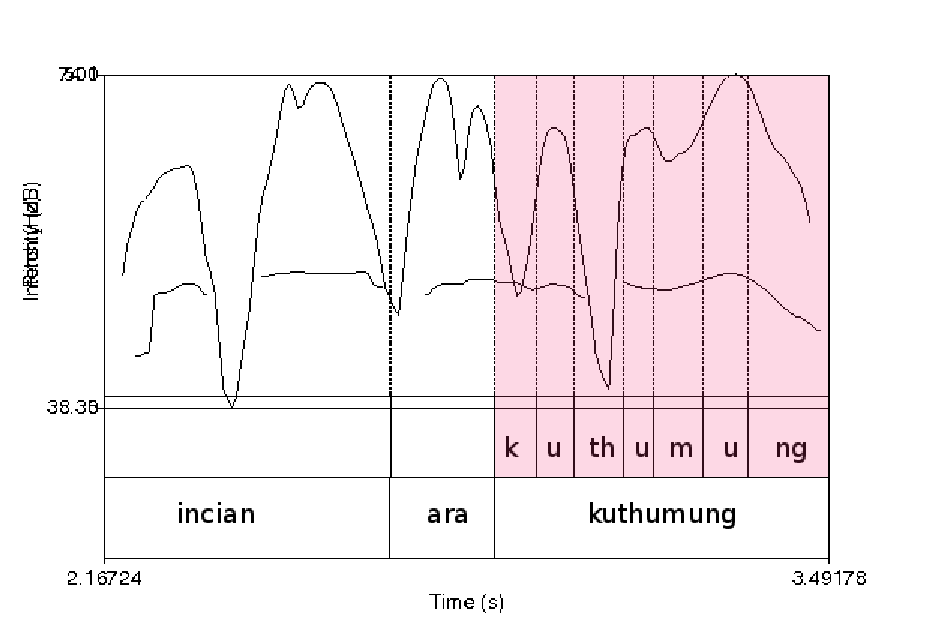
\includegraphics{pics/kuthumungintenspitch.eps}
%  kuthumung-spectro.png: 432x252 pixel, 72dpi, 15.24x8.89 cm, bb=0 0 432 252
 \caption[Absence of pitch and intensity cues for stress in the word \phontrs{ku\dentt umuN}{see}]{Pitch and intensity of an utterance involving the word \phontrs{ku\dentt umuN}{see} show that the first two syllables are not very different in intensity and pitch. Intensity and pitch cannot be used to determine which of the two should be the head. The final syllable has a higher loudness and a raise-fall pitch movement, both of which are the usual way of indicating utterance boundaries of declaratives.}
\label{fig:kuthumungintenspitch}
\end{figure}



Figure \ref{fig:kuthumungintenspitch} shows that neither pitch nor intensity distinguish the first two syllables from each other in the trisyllabic word \phontrs{ku\dentt umu\ng}{see}(The effects on the final syllable are due to the utterance boundary).\footnote{I am aware of the fact that the historical source for this word had two schwas in the first two syllables, so that the lower intensity could be attributed to that.  I do not think that this word has a synchronic schwa, though. The reason for this is that it behaves exactly like trisyllabic words without schwa like \phontrs{makanan}{food}. This word was chosen because it is a monomorphemic trisyllable, of which there are not many. Polymorphemic trisyllables are easier to come by, e.g. nominalizations with \em -an\em. These polymorphemic words were not retained for the recording session  in order to avoid influences that the affixes might have on stress placement. In hindsight, this was a mistake. Future research should include some of these affixes trisyllables as well. I am confident that future research on pitch and intensity will provide no more stress cues for these trisyllables than they did for disyllables or the \textipa{ku\dentt umuN}-type words.} Instrumental analysis of a sample of words with different syllable structures in varying positions within the clause showed that \em ku\dentt umu\ng{} \em is no exception and that pitch and intensity do not provide cues of prominence \citep{ApoussidouEtAl2008}. This lack of word accent is actually not unheard of in the Malay world, as will be discussed in more detail in Section \ref{sec:phon:SLMasastresslesslanguage}.
Another stress cue which some languages use to indicate prominence of a syllable is vowel duration. This is not the case in SLM either. The spectrogram of \em ku\dentt umu\ng{} \em (Figure \ref{fig:kuthumungspectro}) shows that the vowels are of comparable length here (also see Figure \ref{fig:baalasbalasan} for a derived trisyllable). True, there are long and short vowels in SLM, as shown in Section \ref{sec:phon:Vowellength}, but if this was a stress cue, we would expect a difference in vowel duration (or at least moraic weight) to show up in every word, namely on the prominent syllable. This is not the case, as words like \em ku\dentt umu\ng{} \em show. The hypothesis makes wrong predictions, and must be amended or abandoned. A possible amendment would be to state \em Trisyllables of the \em ku\dentt umu\ng{} \em type do not show stress. \em This amendment would have to rely on lexical specification. The fact that there are differences in vowel duration needs explanation nevertheless. In Section \ref{sec:phon:Analysisofwordstructure}, I will argue that vowel duration can better be explained by foot structure, and that this analysis does not need specification in the lexicon and is therefore superior to the ``stress analysis''.


\begin{figure}
 \centering
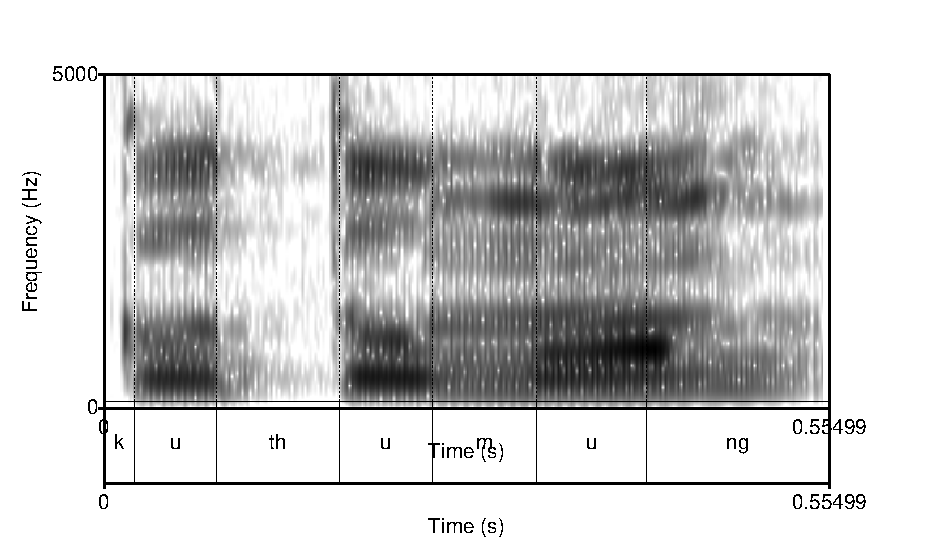
\includegraphics{pics/kuthumung-spectro.eps}
%  kuthumung-spectro.png: 432x252 pixel, 72dpi, 15.24x8.89 cm, bb=0 0 432 252
 \caption[Duration of vowels in \phontrs{ku\dentt umuN}{see}]{The spectrogram of \phontrs{ku\dentt umuN}{see} shows that all three u's are of about equal duration. Duration is therefore not a cue to determine syllable prominence.}
\label{fig:kuthumungspectro}
\end{figure}


The last stress cue which some languages use is vowel quality. Prominent syllables typically show a greater range of possible vowels, whereas non-prominent syllables have a smaller array and might only admit reduced vowels. In SLM, the antepenultimate syllable  of a root seems to be a less prominent syllable, since it only admits  [i], [u] and schwa (the latter often dropped altogether), but not [a], [e] or [o], the most sonorant vowels \citep{Jespersen1904,Selkirk1984,Clements1990sonority}.\footnote{Antepenultimate syllables are often restricted to schwa in Malay varieties, see \citet[12,31,59]{Adelaar1985} for examples of Standard Malay and Jakartanese.} While this is an indication of lack of prominence of this syllable, it does not indicate which of the remaining syllables is most prominent. Furthermore, this lack of prominence of the antepenultimate only applies on the root level; on the stem level, any vowel can be found in antepenultimate position (see Section \ref{sec:phon:struct:Stems}).

To conclude, pitch and intensity do not distinguish syllable prominence in SLM. Differences in vowel duration are not found in all words and are therefore a bad stress cue. Vowel quality finally could indicate lack of prominence of one syllable on the root level. It does not provide positive prominence cues on the stem level, and does not provide any cues on the stem level.


\section{Analysis of word structure}\label{sec:phon:Analysisofwordstructure}
I will argue in this section that the different types of roots we find in SLM and the occurrence of long vowels can be explained by extrametricality of the final syllable \citep{Kiparsky1985lexphon} and a bimoraic foot requirement\footnote{It is interesting to note that Sinhala also parses words into bimoraic feet \citep{Letterman1997}.} \citep{McCarthyEtAl1993}. The list in \xref{list:phon:wordtypes} is repeated and reordered here for convenience.



\setcounter{mycounter}{1}
\ea\label{list:phon:wordtypes2}
\begin{tabular}{@{\arabic{mycounter})\stepcounter{mycounter}~~~~~}ll@{~~~e.g.~~~}l}
&(C)VC$_i$.C$_j$V(C)	 & \phontrs{kumpul}{collect}\\
&(C)VC$_i$.C$_i$V(C)	 & \phontrs{\dentt op:i}{hat}\\
&CV.CV.CV(C)		 & \phontrs{ku\dentt umu\ng}{see}\\
&(C)V\textipa{:}.CV(C)		 & \phontrs{\dentt i:ga}{three}\\
&CV\textipa{:}.GVC		 & \phontrs{\dentt u:\V a}{old} (G=glide)\\
&C\E.CV\textipa{:}.CV(C)		 & \phontrs{c\E ca:\V ak}{wash}\\
&C\E C$_i$.C$_j$V	& \phontrs{m\I \dentn\dentt a}{vomit}\\
&(C)\E C$_j$.C$_j$V(C)	 & \phontrs{s\I g:aR}{healthy}\\
&CV\textipa{:}			 & \phontrs{pi:}{go}, \phontrs{\dentt e:}{tea}\\
&CVC			 & \phontrs{pon}{bride}\\
&(C)V.CV			 & \phontrs{ka\dentt a}{\textsc{quot}}\\
&CVC.CVC.CVC		 & \phontrs{kak:aRla\dentt}{cockroach} (only example)\\

&CV.GVC		 	& \phontrs{lija\dentt}{see}\\

&CV$_i$.h$_i$C		 & \phontrs{poho\ng}{tree}\\
&(\E)N.CVC		 & \phontrs{(\U)mpa\dentt}{four}\\
&(\E)C$_i$.C$_i$V(C)	 & \phontrs{(\U)m:as}{gold}\\
\end{tabular}
\z


\subsection{Roots}\label{sec:phon:analysis:Roots}

The following analytic generalizations can be drawn from this list: Within stems, a penultimate syllable is heavy iff it is not preceded by another syllable containing a full vowel, where heavy syllables are CV\textipa{:} and CVC. I propose that this distribution can be captured by the following principles:

\begin{itemize}
 \item treat final syllables as extrametrical 
 \item build bimoraic feet at right edge of stem
 \item \E{} cannot project a mora \citep{Kager1989}
 \item \I{} and \U{} can project a mora
 \item reduced vowels \phonet{@,I,U} cannot lengthen
\end{itemize}

From these principles, it follows that disyllabic stems lengthen the vowel in an open penultimate syllable to build a bimoraic foot. The same is true for trisyllables with initial schwa. This will be developed below for the different types.

\subsubsection{Canonical cases}\label{sec:phon:Canonicalcasesroots}

A straightforward example of the internal structure of the root is /kumpul/`collect'. This is parsed as /(ku$_{\mu}$m$_{\mu})<$pul$>$/, whose representation is given in \xref{ex:phon:rep:miskin}.

\ea\label{ex:phon:rep:miskin}
\begin{tabular}{lll}
 & ~~~~~~~~~$\omega$\\
 & ~~~~~~/&~ \begin{picture}(0,0)\put(-10,8){\line(1,-3){13}}\end{picture}\\
 & ~~~~F   &  \\
 & ~~~/   &  \\
 &$\sigma$    &$<\sigma>$ \\
 & $\mid$~$\backslash$    & \\
 & $\mu$~$\mu$   &\\
% %  & $\mid$~~~$\mid$&    $\mid$~~~~$\mid$ \\
% C\begin{picture}(0,0)\put(0,10){\line(1,5){8}}\end{picture} & VC~~~C\begin{picture}(0,0)\put(0,10){\line(1,5){8}}\end{picture}   & V  C \\
 & $\mid$~~~$\mid$ & \\
k\begin{picture}(0,0)\put(0,10){\line(1,5){8}}\end{picture} &u~m
&
p\begin{picture}(0,0)\put(-2,10){\line(1,5){8}}\end{picture}
~u\begin{picture}(0,0)\put(-2,10){\line(0,5){40}}\end{picture}
~l\begin{picture}(0,0)\put(-2,10){\line(-1,5){8}}\end{picture}\\
\end{tabular}
\z

We exclude the final syllable \em pul \em and parse the remaining syllable \em kum \em in a bimoraic foot, where the vowel and the coda consonant contribute one mora each.

For disyllables with an underlying geminate, such as \phontrs{\dentt op:i}{hat}, the representation is similar, but the coda consonant of the first syllable serves at the same time as onset of the final syllable.

\ea\label{ex:phon:rep:thoppi}
\begin{tabular}{lll}
 & ~~~~~~~$\omega$\\
 & ~~~~~~/&~ \begin{picture}(0,0)\put(-20,8){\line(1,-3){13}}\end{picture}\\
 & ~~~~F   &  \\
 & ~~~/   &  \\
 &$\sigma$    &\hspace{-0.3cm}$<\sigma>$ \\
 & $\mid$~$\backslash$    & \\
 & $\mu$~$\mu$   &\\
% %  & $\mid$~~~$\mid$&    $\mid$~~~~$\mid$ \\
% C\begin{picture}(0,0)\put(0,10){\line(1,5){8}}\end{picture} & VC~~~C\begin{picture}(0,0)\put(0,10){\line(1,5){8}}\end{picture}   & V  C \\
 & $\mid$~~~~$\backslash$ & \\
\dentt\begin{picture}(0,0)\put(0,10){\line(1,5){8}}\end{picture} & o~~~~~p\begin{picture}(0,0)\put(0,10){\line(1,3){13}}\end{picture}
&
i\begin{picture}(0,0)\put(-2,10){\line(0,5){40}}\end{picture}\\
\end{tabular}
\z


Trisyllabic words like \phontrs{ku\dentt umu\ng}{see} have the foot stretching over two syllables.

\ea\label{ex:phon:rep:kuthumung}
\begin{tabular}{ccc}
 & $\omega$\\
 & /~~~~~& \begin{picture}(0,0)\put(-28,8){\line(2,-3){25}}\end{picture}\\
\multicolumn{2}{c}{~~~~F}&\\
~~~~~/&$\backslash$&\\
~~$\sigma$&~~$\sigma$&$<\sigma>$   \\
~~$\mid$&~~$\mid$&\\
~~~$\mu$&~~~$\mu$&\\
 ~~$\mid$&~~~$\mid$&\\
k\begin{picture}(0,0)\put(-4,10){\line(1,6){7}}\end{picture}~~u &
\dentt\begin{picture}(0,0)\put(-4,10){\line(1,6){7}}\end{picture}~~u&
m\begin{picture}(0,0)\put(-2,10){\line(1,5){8}}\end{picture}
~u\begin{picture}(0,0)\put(-2,10){\line(0,5){40}}\end{picture}
~\ng\begin{picture}(0,0)\put(-2,10){\line(-1,5){8}}\end{picture}\\
\end{tabular}
\z

In disyllables without coda consonant in the penultimate, like \phontrs{\dentt i:ga}{three} \xref{ex:phon:rep:thiiga}, the vowel is lengthened to contribute the second mora for the bimoraic foot.

\ea\label{ex:phon:rep:thiiga}
\begin{tabular}{lll}
 & ~~~~~~~~~$\omega$\\
 & ~~~~~~/&~ \begin{picture}(0,0)\put(-10,8){\line(1,-3){13}}\end{picture}\\
 & ~~~~F   &  \\
 & ~~~/   &  \\
 &$\sigma$    &$<\sigma>$ \\
 & $\mid$~$\backslash$    & \\
 & $\mu$~$\mu$   &\\
% %  & $\mid$~~~$\mid$&    $\mid$~~~~$\mid$ \\
% C\begin{picture}(0,0)\put(0,10){\line(1,5){8}}\end{picture} & VC~~~C\begin{picture}(0,0)\put(0,10){\line(1,5){8}}\end{picture}   & V  C \\
 & $\backslash$~/ & \\
\dentt\begin{picture}(0,0)\put(0,10){\line(1,5){8}}\end{picture}&
 ~~i&
g\begin{picture}(0,0)\put(-2,10){\line(1,5){8}}\end{picture}
~a\begin{picture}(0,0)\put(-2,10){\line(0,5){40}}\end{picture}\\
\end{tabular}
\z

For one set of lexemes with a glide as the onset of the final syllable, the representation is the same as for \phonet{\dentt i:ga}, just above. The word \phontrs{\dentt u:\V a}{old} has an identical representation \xref{ex:phon:rep:thuuva} to \phonet{\dentt i:ga} above.\footnote{This contrasts with a more problematic case for \phontrs{\dentt u\V an}{gentleman}, shown below in \xref{ex:phon:rep:thuvan}.}

\ea\label{ex:phon:rep:thuuva}
\begin{tabular}{lll}
 & ~~~~~~~~~$\omega$\\
 & ~~~~~~/&~ \begin{picture}(0,0)\put(-10,8){\line(1,-3){13}}\end{picture}\\
 & ~~~~F   &  \\
 & ~~~/   &  \\
 &$\sigma$    &$<\sigma>$ \\
 & $\mid$~$\backslash$    & \\
 & $\mu$~$\mu$   &\\
% %  & $\mid$~~~$\mid$&    $\mid$~~~~$\mid$ \\
% C\begin{picture}(0,0)\put(0,10){\line(1,5){8}}\end{picture} & VC~~~C\begin{picture}(0,0)\put(0,10){\line(1,5){8}}\end{picture}   & V  C \\
 & $\backslash$~/ & \\
\dentt\begin{picture}(0,0)\put(0,10){\line(1,5){8}}\end{picture}&
 ~~u&
\V\begin{picture}(0,0)\put(-2,10){\line(1,5){8}}\end{picture}
~a\begin{picture}(0,0)\put(-2,10){\line(0,5){40}}\end{picture}\\
\end{tabular}
\z

In trisyllables with an initial schwa and an open penultimate like \phontrs{c\E ca:\V ak}{wash}, the vowel in the penultimate is also lengthened. This indicates that \E{} does not project a mora \citep[cf.][]{Kager1989}. The foot is then constructed only with the material of the penultimate syllable, which means that the vowel of this syllable needs to be lengthened.

\ea\label{ex:phon:rep:cEcaavak}
	\begin{tabular}{llll}
	& ~~~~$\omega$\\
	& \begin{picture}(0,0)\put(8,8){\line(-1,-2){20}}\end{picture}~~~~~$\mid$&    \begin{picture}(0,0)\put(-10,8){\line(1,-2){20}}\end{picture}\\
	\multicolumn{2}{r}{F~~~~}&\\
		& ~~~~$\mid$ \\
	~~~~$\sigma$ & ~~~~$\sigma$&$<\sigma>$   \\
	& ~~~~$\mid$~$\backslash$    & \\
	& ~~~~$\mu$~$\mu$   & \\
	& ~~~ $\backslash$~/&\\
c\begin{picture}(0,0)\put(-2,10){\line(1,5){8}}\end{picture}
~\E\begin{picture}(0,0)\put(-2,10){\line(0,5){40}}\end{picture}&
c\begin{picture}(0,0)\put(-4,10){\line(1,5){8}}\end{picture}
~~a &
\V\begin{picture}(0,0)\put(-2,10){\line(1,5){8}}\end{picture}
~a\begin{picture}(0,0)\put(-2,10){\line(0,5){40}}\end{picture}
~k\begin{picture}(0,0)\put(-2,10){\line(-1,5){8}}\end{picture}\\
	\end{tabular}
\z

If schwa occurs in a disyllabic like \phontrs{m\I \dentn\dentt a}{ask}, schwa is realized as \I{}, which, unlike \E,  can project a mora. This raising of schwa is then a result of the need for an additional mora, since the coda consonant (in this case /n/)  only provides one, not enough to construct a bimoraic foot.


\ea\label{ex:phon:rep:mIntha}
\begin{tabular}{lll}
 & ~~~~~~~~~$\omega$\\
 & ~~~~~~/&~ \begin{picture}(0,0)\put(-10,8){\line(1,-3){13}}\end{picture}\\
 & ~~~~F   &  \\
 & ~~~/   &  \\
 &$\sigma$    &$<\sigma>$ \\
 & $\mid$~$\backslash$    & \\
 & $\mu$~$\mu$   &\\
% %  & $\mid$~~~$\mid$&    $\mid$~~~~$\mid$ \\
% C\begin{picture}(0,0)\put(0,10){\line(1,5){8}}\end{picture} & VC~~~C\begin{picture}(0,0)\put(0,10){\line(1,5){8}}\end{picture}   & V  C \\
 & $\mid$~~~$\mid$ & \\
m\begin{picture}(0,0)\put(0,10){\line(1,5){8}}\end{picture} & \I~~~\dentn
&
\dentt\begin{picture}(0,0)\put(-2,10){\line(1,5){8}}\end{picture}
~a\begin{picture}(0,0)\put(-2,10){\line(0,5){40}}\end{picture}\\
\end{tabular}
\z

If the initial syllable of a disyllabic word contains schwa in an open syllable, moraic content is neither present in the vowel, since \E{} does not have moraic content, nor in the coda, which is absent. In this case, two things happen: \E{} is raised to \I{}, which does project one mora, and the onset of the following syllable is geminated, yielding a coda, and thereby an additional mora.

\ea\label{ex:phon:rep:sIggar}
\begin{tabular}{lll}
 & ~~~~~~~$\omega$\\
 & ~~~~~~/&~ \begin{picture}(0,0)\put(-20,8){\line(1,-3){13}}\end{picture}\\
 & ~~~~F   &  \\
 & ~~~/   &  \\
 &$\sigma$    &\hspace{-0.3cm}$<\sigma>$ \\
 & $\mid$~$\backslash$    & \\
 & $\mu$~$\mu$   &\\
% %  & $\mid$~~~$\mid$&    $\mid$~~~~$\mid$ \\
% C\begin{picture}(0,0)\put(0,10){\line(1,5){8}}\end{picture} & VC~~~C\begin{picture}(0,0)\put(0,10){\line(1,5){8}}\end{picture}   & V  C \\
 & $\mid$~~~~$\backslash$ & \\
s\begin{picture}(0,0)\put(0,10){\line(1,5){8}}\end{picture} & \I~~~~~g\begin{picture}(0,0)\put(0,10){\line(1,2){20}}\end{picture}
&
a\begin{picture}(0,0)\put(-2,10){\line(0,5){40}}\end{picture}
~r\begin{picture}(0,0)\put(-2,10){\line(-1,5){8}}\end{picture}\\
\end{tabular}
\z



There are only a handful of monosyllabic lexical words such as \phontrs{pi:}{go}, \phontrs{pon}{bride} and \phontrs{\dentt aj}{excrement}. Additionally, there are the pronouns \phontrs{se:}{\textsc{1s.polite}}, \phontrs{go:}{\textsc{1s.familiar}},  \phontrs{lu:}{\textsc{2s.familiar}},  \phontrs{de:}{\textsc{3s.familiar}}.
The fact that all monosyllables have a heavy syllable, especially the long vowel in \textipa{pi:} suggests that the final syllable is not treated as extrametrical for these words. Instead, the bimoraic foot is constructed over the whole word.


\xbox{5}{
\ea\label{ex:phon:rep:pii}
\begin{tabular}{ccc}
 &$\omega$\\
 &$\mid$&\\
 &F   &  \\
 & $\mid$ &  \\
 &$\sigma$    &  \\
 & $\mid$~$\backslash$    & \\
 & $\mu$~$\mu$   &\\
% %  & $\mid$~~~$\mid$&    $\mid$~~~~$\mid$ \\
% C\begin{picture}(0,0)\put(0,10){\line(1,5){8}}\end{picture} & VC~~~C\begin{picture}(0,0)\put(0,10){\line(1,5){8}}\end{picture}   & V  C \\
 & $\backslash$~/ & \\
p\begin{picture}(0,0)\put(0,10){\line(1,4){10}}\end{picture}&
 ~~i&\\
\end{tabular}
\z
} 
\xbox{5}{
\ea\label{ex:phon:rep:pon}
\begin{tabular}{ccc}
 &$\omega$\\
 &$\mid$&\\
 &F   &  \\
 & $\mid$ &  \\
 &$\sigma$    &  \\
 & $\mid$~$\backslash$    & \\
 & $\mu$~$\mu$   &\\
% %  & $\mid$~~~$\mid$&    $\mid$~~~~$\mid$ \\
% C\begin{picture}(0,0)\put(0,10){\line(1,5){8}}\end{picture} & VC~~~C\begin{picture}(0,0)\put(0,10){\line(1,5){8}}\end{picture}   & V  C \\
 & $\mid$~~~$\mid$ & \\
p\begin{picture}(0,0)\put(0,10){\line(1,4){10}}\end{picture}&
o~~n&\\
\end{tabular}
\z
} \\

No function word has a long vowel, even not in penultimate open syllables. This suggests that function words are not subject to the bimoraic foot requirement, and are probably not parsed into a foot nor a word. \xref{ex:phon:rep:katha} shows this for the quotative \em ka\dentt a\em. In this representation, the levels of word, foot and mora are left out, since they are irrelevant for the word \em ka\dentt a\em. 

\xbox{7}{
\ea\label{ex:phon:rep:katha}
\begin{tabular}{cc}
~~  $\sigma$ &~$\sigma$\vspace{0,3cm} \\\\\\
k \begin{picture}(0,0)\put(-2,10){\line(1,5){8}}\end{picture}
~~ 
~a\begin{picture}(0,0)\put(-2,10){\line(-1,5){8}}\end{picture}
&
\dentt \begin{picture}(0,0)\put(-2,10){\line(1,5){8}}\end{picture}
~~ 
~a\begin{picture}(0,0)\put(-2,10){\line(-1,5){8}}\end{picture}\\
\end{tabular}
\z
}


Trisyllabic roots with closed syllables are rare. Only one could be found, \phontrs{kak:aRla\dentt}{cockroach}. It is not clear as of now whether this root is parsed into one bimoraic foot, disregarding the first syllable \xref{ex:phon:rep:kakkarlath1}, or into two feet, as in \xref{ex:phon:rep:kakkarlath2}.



\xbox{7}{
\ea\label{ex:phon:rep:kakkarlath1}
\begin{tabular}{lll}
  	& ~~~$\omega$\\
	&\begin{picture}(0,0)\put(3,8){\line(-1,-2){20}}\end{picture}~~~~$\mid$~~~~~& \begin{picture}(0,0)\put(-23,8){\line(2,-3){25}}\end{picture}\\
~~~~~~~~ &~~~~F&\\
~~~~~~~&  ~~~~$\mid$&\\
~~~~~$\sigma$&~~~~$\sigma$&$<\sigma>$   \\
&~~~~$\mid$ $\backslash$&\\
&~~~~$\mu$~~$\mu$&\\
&~~~ $\mid$~~~$\mid$&\\

k\begin{picture}(0,0)\put(-2,10){\line(1,5){8}}\end{picture}
~a\begin{picture}(0,0)\put(-2,10){\line(0,5){40}}\end{picture}
 &
k\begin{picture}(0,0)\put(-7,10){\line(-1,2){20}}\put(-5,10){\line(1,6){7}}\end{picture}~
a~~r&
l\begin{picture}(0,0)\put(-2,10){\line(1,5){8}}\end{picture}
~a\begin{picture}(0,0)\put(-2,10){\line(0,5){40}}\end{picture}
~\dentt\begin{picture}(0,0)\put(-2,10){\line(-1,5){8}}\end{picture}\\
\end{tabular}
\z
} 
\xbox{7}{
\ea\label{ex:phon:rep:kakkarlath2}
\begin{tabular}{lll}
  	& ~~$\omega$\\
	&\begin{picture}(0,0)\put(-2,8){\line(-2,-3){8}}\end{picture}~~~~$\mid$~~~~~& \begin{picture}(0,0)\put(-23,8){\line(2,-3){25}}\end{picture}\\
~~~~~~~~F &~~~~F&\\
~~~~~~~/&  ~~~~$\mid$&\\
~~~~~$\sigma$&~~~~$\sigma$&$<\sigma>$   \\
~~~~~$\mid$ $\backslash$&~~~~$\mid$ $\backslash$&\\
~~~~$\mu$~$\mu$&~~~~$\mu$~~$\mu$&\\
~~~~~$\mid$&~~~ $\mid$~~~$\mid$&\\
k\begin{picture}(0,0)\put(-2,10){\line(1,6){7}}\end{picture}~~
a &
k\begin{picture}(0,0)\put(-7,10){\line(-1,1){14}}\put(-5,10){\line(1,6){7}}\end{picture}~
a~~r&
l\begin{picture}(0,0)\put(-2,10){\line(1,5){8}}\end{picture}
~a\begin{picture}(0,0)\put(-2,10){\line(0,5){40}}\end{picture}
~\dentt\begin{picture}(0,0)\put(-2,10){\line(-1,5){8}}\end{picture}\\
\end{tabular}
\z
}

\subsubsection{Problematic cases}\label{sec:phon:Problematiccases}


A more problematic case for this analysis are co-occurrence of empty coda and empty onset. Our analysis would predict that for words of the form /CV$_i$V$_j$C/, we get [CV$_i$:V$_j$C] \xref{ex:phon:rep:liiath}. However, what we find is [CV$_i$GV$_j$C] where G is a glide. This newly formed glide is  resyllabified to the onset of the following syllable, yielding [CV$_i$.GV$_j$C]. This resyllabification means that the glide can no longer be the coda, unless it is geminated, which is not the case here. With the coda disappearing, the mora also goes, leaving insufficient material to construct a foot. This is illustrated in \xref{ex:phon:rep:liiath} and \xref{ex:phon:rep:thuuan}.


\xbox{7}{
\ea\label{ex:phon:rep:liiath}*
\begin{tabular}{ll}
 & ~~~~~~$\omega$\\
 & ~~~~~~/~ \begin{picture}(0,0)\put(0,8){\line(1,-3){13}}\end{picture}\\
 & ~~~~F     \\
 & ~~~/     \\
 &$\sigma$ ~~~~ $<\sigma>$ \\
 & $\mid$~$\backslash$     \\
 & $\mu$~$\mu$   \\
 & ~$\backslash$  $\mid$  \\
~*l\begin{picture}(0,0)\put(0,10){\line(1,5){8}}\end{picture}&
 ~~~
i~
~~~~~a\begin{picture}(0,0)\put(-2,10){\line(0,5){40}}\end{picture}
~\dentt\begin{picture}(0,0)\put(-2,10){\line(-1,5){8}}\end{picture}~~(=\phonet{li:a\dentt})\\
\end{tabular}
\z
}
\xbox{7}{
\ea\label{ex:phon:rep:liyath}
\begin{tabular}{ll}
 & ~~~~~~$\omega$\\
 & ~~~~~~/~ \begin{picture}(0,0)\put(0,8){\line(1,-3){13}}\end{picture}\\
 & ~~~~F?     \\
 & ~~~/     \\
 &$\sigma$ ~~~~ $<\sigma>$ \\
 & $\mid$~?     \\
 & $\mu$~$\mu$?   \\
 & ~$\backslash$  ?  \\
l\begin{picture}(0,0)\put(0,10){\line(1,5){8}}\end{picture}&
 ~~~
i~\begin{picture}(0,0)\put(0,12){\line(2,5){15}}\end{picture}
~~~~~a\begin{picture}(0,0)\put(-2,10){\line(0,5){40}}\end{picture}
~\dentt\begin{picture}(0,0)\put(-2,10){\line(-1,5){8}}\end{picture}~~(=\phonet{lija\dentt})\\
\end{tabular}
\z
}

\xbox{7}{
\ea\label{ex:phon:rep:thuuan}*
\begin{tabular}{ll}
 & ~~~~~~$\omega$\\
 & ~~~~~~/~ \begin{picture}(0,0)\put(0,8){\line(1,-3){13}}\end{picture}\\
 & ~~~~F     \\
 & ~~~/     \\
 &$\sigma$ ~~~~ $<\sigma>$ \\
 & $\mid$~$\backslash$     \\
 & $\mu$~$\mu$   \\
 & ~$\backslash$  $\mid$  \\
~*\dentt\begin{picture}(0,0)\put(0,10){\line(1,5){8}}\end{picture}&
 ~~~
u~
~~~~~a\begin{picture}(0,0)\put(-2,10){\line(0,5){40}}\end{picture}
~n\begin{picture}(0,0)\put(-2,10){\line(-1,5){8}}\end{picture}~~(=\phonet{\dentt u:an})\\
\end{tabular}
\z
}
\xbox{7}{
\ea\label{ex:phon:rep:thuvan}
\begin{tabular}{ll}
 & ~~~~~~$\omega$\\
 & ~~~~~~/~ \begin{picture}(0,0)\put(0,8){\line(1,-3){13}}\end{picture}\\
 & ~~~~F?     \\
 & ~~~/     \\
 &$\sigma$ ~~~~ $<\sigma>$ \\
 & $\mid$~?     \\
 & $\mu$~$\mu$?   \\
 & ~$\backslash$  ?  \\
\dentt\begin{picture}(0,0)\put(0,10){\line(1,5){8}}\end{picture}&
 ~~~
u~\begin{picture}(0,0)\put(0,12){\line(2,5){15}}\end{picture}
~~~~~a\begin{picture}(0,0)\put(-2,10){\line(0,5){40}}\end{picture}
~n\begin{picture}(0,0)\put(-2,10){\line(-1,5){8}}\end{picture}~~(=\phonet{\dentt u\V an})\\
\end{tabular}
\z
}





Under derivational accounts, it is easy to formulate a rule like
% 
% \ea $\begin{array}{c}[+vocalic]\\[\pm front]\end{array}:\to\begin{array}{c}[+vocalic]\\[\pm front]\end{array}\begin{array}{c}[-vocalic]\\[\pm front]\end{array}$\_V\z

\ea $[+vocalic]$\textipa{:}$ \to [+vocalic][-vocalic]/\_[+vocalic]$\z

In other words, a long vowel is split into a vowel and a glide before another vowel. It is unclear as of now how this could be made to work with the general foot structure.

The problem with words of the structure CV$_i$.hV$_i$C	like \phontrs{poho\ng}{tree} is similar. A vowel preceding the same vowel, separated by an /h/ is never lengthened. \citet{Tapovanaye1995} assumes that these words have the underlying form /CV$_i$V$_i$C/ and that an h is inserted to prevent hiatus. Crucially, this takes place after vowel lengthening. In such a derivational account, this can be formulated as

\ea V$_i$\textipa{:} $\to$ V$_i$h/\_V$_i$\z

This phenomenon cannot be captured with the analysis presented there. The bimoraic foot cannot be constructed for these words. On the other hand, the derivational account presented by Tapovanaye is not very plausible either, since the insertion of an h instead of a glide is not very well motivated, and historically, an h is present in these words anyway. 

Another problem for the foot structure assumed in this analysis is the deletion of schwa between empty onset and nasals as in \phonem{@mpa\dentt}, which can be pronounced \phonet{Umpa\dentt}, but also \phonet{\s{m}pa\dentt}. For the first pronunciation, there is no problem \xref{ex:phon:rep:umpath}, but if the raised schwa is deleted, as is the case in the second pronunciation, a mora disappears and no bimoraic foot can be constructed. Whether the final syllable should be extrametrical \xref{ex:phon:rep:mpath1} or not \xref{ex:phon:rep:mpath2} is unclear as of now.



\xbox{5}{
\ea\label{ex:phon:rep:umpath}
\begin{tabular}{lll}
 & ~~~~~~~~~$\omega$\\
 & ~~~~~~/&~ \begin{picture}(0,0)\put(-10,8){\line(1,-3){13}}\end{picture}\\
 & ~~~~F   &  \\
 & ~~~/   &  \\
 &$\sigma$    &$<\sigma>$ \\
 & $\mid$~$\backslash$    & \\
 & $\mu$~$\mu$   & \\
% %  & $\mid$~~~$\mid$&    $\mid$~~~~$\mid$ \\
% C\begin{picture}(0,0)\put(0,10){\line(1,5){8}}\end{picture} & VC~~~C\begin{picture}(0,0)\put(0,10){\line(1,5){8}}\end{picture}   & V  C \\
 & $\mid$~~~$\mid$ & \\
 & \U~~~m
&
p\begin{picture}(0,0)\put(-2,10){\line(1,5){8}}\end{picture}
~a\begin{picture}(0,0)\put(-2,10){\line(0,5){40}}\end{picture}
~\dentt\begin{picture}(0,0)\put(-2,10){\line(-1,5){8}}\end{picture}\\
\end{tabular}
\z
}
\xbox{5}{
\ea\label{ex:phon:rep:mpath1}
\begin{tabular}{lll}
 & ~~~~~~~~~$\omega$\\
 & ~~~~~~&\begin{picture}(0,0)\put(-25,8){\line(-1,-3){13}}\end{picture} \begin{picture}(0,0)\put(-10,8){\line(1,-3){13}}\end{picture}\\
 & ~~~~  &  \\
 & ~~~   &  \\
 &$\sigma$    &$<\sigma>$ \\
 & $\mid$   & \\
 & $\mu$?   &\\
% %  & $\mid$~~~$\mid$&    $\mid$~~~~$\mid$ \\
% C\begin{picture}(0,0)\put(0,10){\line(1,5){8}}\end{picture} & VC~~~C\begin{picture}(0,0)\put(0,10){\line(1,5){8}}\end{picture}   & V  C \\
 & $\mid$  & \\
 & \textipa{\s{m}}
&
p\begin{picture}(0,0)\put(-2,10){\line(1,5){8}}\end{picture}
~a\begin{picture}(0,0)\put(-2,10){\line(0,5){40}}\end{picture}
~\dentt\begin{picture}(0,0)\put(-2,10){\line(-1,5){8}}\end{picture}\\
\end{tabular}
\z
}
\xbox{5}{
\ea\label{ex:phon:rep:mpath2}
\begin{tabular}{lll}
 & ~~~~~~~~~$\omega$\\
 & ~~~~~~&\begin{picture}(0,0)\put(-25,8){\line(-1,-3){13}}\end{picture}
\begin{picture}(0,0)\put(-10,8){\line(1,-3){4}}\end{picture} \\
 & ~~~~  & F \\
 & ~~~   &~ $\backslash$ \\
 &$\sigma$    &~~~$\sigma$ \\
 &       &~~~~$\mid$ $\backslash$ \\
 &       & ~~~~$\mu$~$\mu$  \\
 &   &~~~~$\mid$ ~ $\mid$  \\
 & \textipa{\s{m}}\begin{picture}(0,0)\put(-5,10){\line(0,5){40}}\end{picture}
&
p\begin{picture}(0,0)\put(-4,10){\line(1,5){8}}\end{picture}
~a 
~\dentt \\
\end{tabular}
\z
}

For the very last type in list \xref{list:phon:wordtypes2}, the (\E)C$_i$C$_i$V(C) type represented by \phontrs{Um:as}{gold}, the discussion is analogous to \phontrs{Umpa\dentt}{four}.


\xbox{5}{
\ea\label{ex:phon:rep:ummas}
\begin{tabular}{lll}
 & ~~~~~~~~~$\omega$\\
 & ~~~~~~/&~ \begin{picture}(0,0)\put(-10,8){\line(1,-3){13}}\end{picture}\\
 & ~~~~F   &  \\
 & ~~~/   &  \\
 &$\sigma$    &$<\sigma>$ \\
 & $\mid$~$\backslash$    & \\
 & $\mu$~$\mu$   &\\
% %  & $\mid$~~~$\mid$&    $\mid$~~~~$\mid$ \\
% C\begin{picture}(0,0)\put(0,10){\line(1,5){8}}\end{picture} & VC~~~C\begin{picture}(0,0)\put(0,10){\line(1,5){8}}\end{picture}   & V  C \\
 & $\mid$~~~$\backslash$ & \\
 & \U~~~m\begin{picture}(0,0)\put(2,10){\line(2,3){27}}\end{picture}
&
~
~a\begin{picture}(0,0)\put(-2,10){\line(0,5){40}}\end{picture}
~s\begin{picture}(0,0)\put(-2,10){\line(-1,5){8}}\end{picture}\\
\end{tabular}
\z
}
\xbox{5}{
\ea\label{ex:phon:rep:mmas1}
\begin{tabular}{ll}
 & ~ ~$\omega$\\
 &\begin{picture}(0,0)\put(10,8){\line(-1,-6){7}}\end{picture} \begin{picture}(0,0)\put(10,8){\line(1,-3){13}}\end{picture}\\
 ~~~~  &  \\
 ~~~   &  \\
 &$\sigma$ ~   $<\sigma>$ \\
 & $\mid$   \\
 & $\mu$?  \\
 &  $\mid$ \\
 &m \begin{picture}(0,0)\put(-2,10){\line(1,3){13}}\end{picture}
~
~a\begin{picture}(0,0)\put(-2,10){\line(0,5){40}}\end{picture}
~s\begin{picture}(0,0)\put(-2,10){\line(-1,5){8}}\end{picture}\\
\end{tabular}
\z
}
\xbox{5}{
\ea\label{ex:phon:rep:mmas2}
\begin{tabular}{ll}
 & ~ ~$\omega$\\
 &\begin{picture}(0,0)\put(10,8){\line(-1,-6){7}}\end{picture}
\begin{picture}(0,0)\put(12,8){\line(1,-3){4}}\end{picture} \\
 & ~~~~~~   F \\
 & ~~~ ~   ~ $\backslash$ \\
 &$\sigma$  ~~~ $\sigma$ \\
 &  ~ ~~~~~~ $\mid$ $\backslash$   \\
 &  ~ ~~~~~$\mu$~~$\mu$ \\
 &  ~  ~~~~~ $\mid$  ~~ $\mid$ \\
 &m \begin{picture}(0,0)\put(-10,10){\line(0,5){40}}\put(-2,10){\line(1,3){13}}\end{picture}
~
~a 
~~s \\
\end{tabular}
\z
}



\subsection{Stems}\label{sec:phon:analysis:Stems}
Stems consist of an obligatory root and optionally additional roots or derivational morphemes.

There are only a handful of monosyllabic roots, which do not combine well with each other nor with the derivational morphemes. This means that all bimorphemic stems have at least one disyllabic root, which makes the complex stems at least trisyllabic. These polysyllabic stems respond to the same criteria as roots, i.e. extrametricality of the final syllable and construction of a bimoraic foot.

\subsubsection{Canonical cases}\label{sec:phon:Canonicalcasesstems}

The additional material provided by the derivational affix or the second root in the compound means that more moraic content is available, and that strategies to provide missing moraic content, like vowel lengthening, gemination, or raising of schwa are less necessary with complex stems than with roots.
If, through affixation or compounding, other possibilities to construct bimoraic feet arise, the vowel of the penultimate is not lengthened.  The syllable containing the suffix becomes extrametrical, and the formerly extrametric final syllable now is penultimate and can provide moraic content. \phontrs{(ma$_\mu$ka$_\mu$)$<$nan$>$}{food} has two moraic vowels in the first two syllable, canceling the need for an additional vowel for the second mora, which is necessary in \phontrs{(ma$_\mu$:$_\mu$)$<$ka\ng$>$}{eat}. Both representations are given in \xref{ex:phon:rep:maakang} and \xref{ex:phon:rep:makanan}

\xbox{7}{
\ea\label{ex:phon:rep:maakang}
\begin{tabular}{lll}
 & ~~~~~~~~~$\omega$\\
 & ~~~~~~/&~ \begin{picture}(0,0)\put(-10,8){\line(1,-3){13}}\end{picture}\\
 & ~~~~F   &  \\
 & ~~~/   &  \\
 &$\sigma$    &$<\sigma>$ \\
 & $\mid$~$\backslash$    & \\
 & $\mu$~$\mu$   &\\
% %  & $\mid$~~~$\mid$&    $\mid$~~~~$\mid$ \\
% C\begin{picture}(0,0)\put(0,10){\line(1,5){8}}\end{picture} & VC~~~C\begin{picture}(0,0)\put(0,10){\line(1,5){8}}\end{picture}   & V  C \\
 & $\backslash$~/ & \\
m\begin{picture}(0,0)\put(0,10){\line(1,5){8}}\end{picture}&
 ~~a&
k\begin{picture}(0,0)\put(-2,10){\line(1,5){8}}\end{picture}
~a\begin{picture}(0,0)\put(-2,10){\line(0,5){40}}\end{picture}
~\ng\begin{picture}(0,0)\put(-2,10){\line(-1,5){8}}\end{picture}\\
\end{tabular}
\z
}
\xbox{7}{
\ea\label{ex:phon:rep:makanan}
\begin{tabular}{ccc}
 & $\omega$\\
 & /~~~~~& \begin{picture}(0,0)\put(-28,8){\line(2,-3){25}}\end{picture}\\
\multicolumn{2}{c}{~~~~F}&\\
~~~~~/&$\backslash$&\\
~~$\sigma$&~~$\sigma$&$<\sigma>$   \\
~~$\mid$&~~$\mid$&\\
~~~$\mu$&~~~$\mu$&\\
~~~$\mid$&~~~$\mid$&\\
m\begin{picture}(0,0)\put(-4,10){\line(1,6){7}}\end{picture}~~a &
k\begin{picture}(0,0)\put(-4,10){\line(1,6){7}}\end{picture}~~a&
n\begin{picture}(0,0)\put(-2,10){\line(1,5){8}}\end{picture}
~a\begin{picture}(0,0)\put(-2,10){\line(0,5){40}}\end{picture}
~n\begin{picture}(0,0)\put(-2,10){\line(-1,5){8}}\end{picture}\\
\end{tabular}
\z
}

For disyllables with schwa in open syllables, material provided by affixes cancels the need for one extra mora. This means that gemination is no longer necessary, while realizing schwa as \phonet{I} is. The representations in  \xref{ex:phon:rep:sIgaran} show the difference in gemination between the disyllable and the nominalized  trisyllable.

\ea\label{ex:phon:rep:sIgaran}
\begin{tabular}{ccc}
\begin{tabular}{lll}
 & ~~~~~~~$\omega$\\
 & ~~~~~~/&~ \begin{picture}(0,0)\put(-20,8){\line(1,-3){13}}\end{picture}\\
 & ~~~~F   &  \\
 & ~~~/   &  \\
 &$\sigma$    &\hspace{-0.3cm}$<\sigma>$ \\
 & $\mid$~$\backslash$    & \\
 & $\mu$~$\mu$   &\\
% %  & $\mid$~~~$\mid$&    $\mid$~~~~$\mid$ \\
% C\begin{picture}(0,0)\put(0,10){\line(1,5){8}}\end{picture} & VC~~~C\begin{picture}(0,0)\put(0,10){\line(1,5){8}}\end{picture}   & V  C \\
 & $\mid$~~~~$\backslash$ & \\
s\begin{picture}(0,0)\put(0,10){\line(1,5){8}}\end{picture} & \I~~~~~g\begin{picture}(0,0)\put(0,10){\line(1,2){20}}\end{picture}
&
a\begin{picture}(0,0)\put(-2,10){\line(0,5){40}}\end{picture}
~r\begin{picture}(0,0)\put(-2,10){\line(-1,5){8}}\end{picture}\\
\end{tabular}
&
\hspace{1cm}
&
\begin{tabular}{ccc}
 & $\omega$\\
 & /~~~~~& \begin{picture}(0,0)\put(-28,8){\line(2,-3){25}}\end{picture}\\
\multicolumn{2}{c}{~~~~F}&\\
~~~~~/&$\backslash$&\\
~~$\sigma$&~~$\sigma$&$<\sigma>$   \\
~~$\mid$&~~$\mid$&\\
~~$\mu$&~~$\mu$&\\
~$\mid$&~$\mid$&\\
s\begin{picture}(0,0)\put(-4,10){\line(1,6){7}}\end{picture}~~\I &
g\begin{picture}(0,0)\put(-4,10){\line(1,6){7}}\end{picture}~~a&
r\begin{picture}(0,0)\put(-2,10){\line(1,5){8}}\end{picture}
~a\begin{picture}(0,0)\put(-2,10){\line(0,5){40}}\end{picture}
~n\begin{picture}(0,0)\put(-2,10){\line(-1,5){8}}\end{picture}\\
\end{tabular}
\end{tabular}
\z

Another logical possibility would be to realize schwa as \phonet{@} and geminate the onset of the final syllable. This would also provide an extra mora, but this solution is not employed. All geminated roots lose their gemination when nominalized.



The derivational suffix \em -blas \em is used to derive the numbers from thirteen to nineteen. It behaves like \em -an \em in the sense that it is parsed into the same phonological word as its host, which allows the formerly extrametrical final syllable to contribute moraic weight to the bimoraic foot, abolishing the need for vowel lengthening.


\ea\label{ex:phon:rep:thigablas}
\begin{tabular}{ccc}
	\begin{tabular}{lll}
	& ~~~~~~~~~$\omega$\\
	& ~~~~~~/&~ \begin{picture}(0,0)\put(-10,8){\line(1,-3){13}}\end{picture}\\
	& ~~~~F   &  \\
	& ~~~/   &  \\
	&$\sigma$    &$<\sigma>$ \\
	& $\mid$~$\backslash$    & \\
	& $\mu$~$\mu$   &\\
	% %  & $\mid$~~~$\mid$&    $\mid$~~~~$\mid$ \\
	% C\begin{picture}(0,0)\put(0,10){\line(1,5){8}}\end{picture} & VC~~~C\begin{picture}(0,0)\put(0,10){\line(1,5){8}}\end{picture}   & V  C \\
	& $\backslash$~/ & \\
	\dentt\begin{picture}(0,0)\put(0,10){\line(1,5){8}}\end{picture}&
	~~i&
	g\begin{picture}(0,0)\put(-2,10){\line(1,5){8}}\end{picture}
	~a\begin{picture}(0,0)\put(-2,10){\line(0,5){40}}\end{picture}\\
	\end{tabular}
&
\hspace{1cm}
&
	\begin{tabular}{ccc}
	& $\omega$\\
	& /~~~~~& \begin{picture}(0,0)\put(-28,8){\line(2,-3){25}}\end{picture}\\
	\multicolumn{2}{c}{~~~~F}&\\
	~~~~~/&$\backslash$&\\
	~~$\sigma$&~~$\sigma$&$<\sigma>$   \\
	~~$\mid$&~~$\mid$&\\
	~~$\mu$&~~$\mu$&\\
	~$\mid$&~$\mid$&\\
	\dentt\begin{picture}(0,0)\put(-4,10){\line(1,6){7}}\end{picture}~~i &
	g\begin{picture}(0,0)\put(-4,10){\line(1,6){7}}\end{picture}~~a&
	b\begin{picture}(0,0)\put(-2,10){\line(1,5){8}}\end{picture}l\begin{picture}(0,0)\put(-2,10){\line(1,5){8}}\end{picture}
	~a\begin{picture}(0,0)\put(-2,10){\line(0,5){40}}\end{picture}
	~s\begin{picture}(0,0)\put(-2,10){\line(-1,5){8}}\end{picture}\\
	\end{tabular}
\end{tabular}
\z


Compounding, just like affixation, provides extra material and influences the construction of feet and the need or not for additional moras. In \xref{ex:phon:rep:kaca}, the words \phontrs{ka:ca}{mirror} and \phontrs{ma:\dentt a}{eye} are compounded. Both orders are possible, and the resulting meaning is `spectacles' in both cases. The resulting word cannot be parsed into feet exhaustively, which is why the last possible vowel is lengthened, in this case the vowel in the penultimate syllable.

\ea\label{ex:phon:rep:kaca}
\begin{tabular}{ccc}
	\begin{tabular}{lll}
	& ~~~~~~~~~$\omega$\\
	& ~~~~~~/&~ \begin{picture}(0,0)\put(-10,8){\line(1,-3){13}}\end{picture}\\
	& ~~~~F   &  \\
	& ~~~/   &  \\
	&$\sigma$    &$<\sigma>$ \\
	& $\mid$~$\backslash$    & \\
	& $\mu$~$\mu$   &\\
	% %  & $\mid$~~~$\mid$&    $\mid$~~~~$\mid$ \\
	% C\begin{picture}(0,0)\put(0,10){\line(1,5){8}}\end{picture} & VC~~~C\begin{picture}(0,0)\put(0,10){\line(1,5){8}}\end{picture}   & V  C \\
	& $\backslash$~/ & \\
	m\begin{picture}(0,0)\put(0,10){\line(1,5){8}}\end{picture}&
	~~a&
	\dentt\begin{picture}(0,0)\put(-2,10){\line(1,5){8}}\end{picture}
	~a\begin{picture}(0,0)\put(-2,10){\line(0,5){40}}\end{picture}\\
	k&
	~~a&
	c
	~a\\
	\end{tabular}
&
\hspace{1cm}
&
\begin{tabular}{ccllll}
&&&&  $\omega$\\
&\begin{picture}(0,0)\put(-10,0){\line(6,1){56}}\end{picture}&&&$\mid$&\begin{picture}(0,0)\put(-30,8){\line(2,-3){25}}\end{picture}\\
\multicolumn{2}{c}{F}&& &  F   &  \\
\multicolumn{2}{c}{/$\backslash$}&& & $\mid$   &  \\
~~$\sigma$&~~$\sigma$&      & & $\sigma$    &\hspace{-0.5cm}$<\sigma>$ \\
~~$\mid$&~~$\mid$&          & & $\mid$~$\backslash$    & $\mid$\\
~~$\mu$&~~$\mu$&            & & $\mu$~$\mu$   & $\mu$\\
~$\mid$&~$\mid$&            & & $\mid$ /~~~~~ & $\mid$\\
C\begin{picture}(0,0)\put(-4,10){\line(1,6){7}}\end{picture}V & C\begin{picture}(0,0)\put(-4,10){\line(1,6){7}}\end{picture}V &                   &C\begin{picture}(0,0)\put(0,10){\line(1,4){10}}\end{picture}& V~~~~C\begin{picture}(0,0)\put(0,10){\line(1,4){10}}\end{picture}   & V\\
$\mid$~$\mid$&$\mid$~$\mid$ & & $\mid$ & $\mid$~~~~~~$\mid$ & $\mid$\\
ka & ca&                    &m& a~~~~~\dentt   & a\\
ma & \dentt a&                    &k& a~~~~~c   & a\\
\end{tabular}                            
\end{tabular}
\z

\subsubsection{Problematic case}\label{sec:phon:Problematiccase}
The derivational suffix \em -pulu \em is used to derive the numbers from twenty to ninety. The behaviour of this suffix is difficult to accommodate, since it precludes vowel lengthening of the stem, but the resulting word fails parse exhaustively.

\ea
	\ea \dentt$ i_\mu.(ga_\mu.pu_\mu).<lu_\mu>$
	\ex (\dentt$ i_\mu.ga_\mu).pu_\mu.<lu_\mu>$
\z\z

% However, exhaustivity of parsing is not an inviolable constraint \citep{McCarthyEtAl1993}, so that this problem can be regarded as minor.

% Vowel lengthening of the could be used to build bimoraic feet, but the resulting forms are ungrammatical.

% \ea\label{ex:phon:thigapululength}
% 	\ea *(\dentt$ i_\mu\textipa{:}\mu).(ga_\mu.pu_\mu).<lu_\mu>$
% 	\ex *(\dentt$ i_\mu.ga_\mu)(\textipa{:}_\mu.pu_\mu).<lu_\mu>$
% 	\ex *(\dentt$ i_\mu.ga_\mu).(pu_\mu\textipa{:}_\mu).<lu_\mu>$
% \z\z
% 
% % One possible solution would be a constraint that only lexical material may bear long vowels, which is observed elsewhere in the grammar. This would explain why \xref{ex:phon:thigapululength}c. is ungrammatical. Another constraint banning vowel length in syllables preceding the penultimate could be used to rule out \xref{ex:phon:thigapululength}ab, but this seems rather an ad hoc solution. For the time being, the behaviour of \em -pulu \em cannot be explained in a satisfying way.


\subsection{Words}\label{sec:phon:analysis:Words}
Words consist of a stem and optionally inflectional affixes or clitics. This extra material has no influence on the parsing of the stem. Inflectional material is not parsed into the same phonological word as the stem. This means that the representation of the word does not differ much from the representation of the stem. In SLM, there are two main types of extra material for words: verbal prefixes (see Section \ref{sec:morph:Prefixes}) or proclitics (see Sections \ref{sec:morph:Quasi-prefixes} and \ref{sec:morph:Simpleclitics}), and enclitics, which are used for a variety of functions, like case marking, emphasis, coordination, etc. (see Section \ref{sec:morph:Boundwords}).

Prefixes are not parsed into the same phonological word as the stem. Both monosyllabic and disyllabic prefixes behave alike in this regard \xref{ex:phon:rep:prefixes}. The additional material provided by \phontrs{su-}{\textsc{past}}{} or \phontrs{aR\E-}{\textsc{non.past}}{} does not take away the need to lengthen the penultimate syllable to construct the bimoraic foot.

\ea\label{ex:phon:rep:prefixes}
\begin{tabular}{ccc}
	\begin{tabular}{cllll}
	& & ~$\omega$\\
	& &  ~/& \begin{picture}(0,0)\put(-20,8){\line(2,-3){25}}\end{picture}\\
	& &   F   & \\
	& & $\mid$& \\
	~~~$\sigma$& & $\sigma$&$<\sigma>$   \\
	& & $\mid$~$\backslash$    &\\
	& & $\mu$~$\mu$   &\\
	& & $\mid$ /~~~~~ &\\
s\begin{picture}(0,0)\put(-2,10){\line(1,5){8}}\end{picture}
u\begin{picture}(0,0)\put(-2,10){\line(0,5){40}}\end{picture}&
-~m\begin{picture}(0,0)\put(-2,10){\line(1,5){8}}\end{picture} &
a   &
k\begin{picture}(0,0)\put(-2,10){\line(1,5){8}}\end{picture}
~a\begin{picture}(0,0)\put(-2,10){\line(0,5){40}}\end{picture}
~\ng\begin{picture}(0,0)\put(-2,10){\line(-1,5){8}}\end{picture}\\
	\end{tabular}
&
\hspace{2cm}
&
	\begin{tabular}{cllll}
	& & ~$\omega$\\
	& &  ~/& \begin{picture}(0,0)\put(-20,8){\line(2,-3){25}}\end{picture}\\
	& &   F   & \\
	& & $\mid$& \\
	~$\sigma$~~~$\sigma$& & $\sigma$&$<\sigma>$   \\
	& & $\mid$~$\backslash$    &\\
	& & $\mu$~$\mu$   &\\
	& & $\mid$ /~~~~~ &\\
a\begin{picture}(0,0)\put(-2,10){\line(0,5){40}}\end{picture}
~r\begin{picture}(0,0)\put(-2,10){\line(1,5){8}}\end{picture}
\E\begin{picture}(0,0)\put(-2,10){\line(0,5){40}}\end{picture}&
-~m\begin{picture}(0,0)\put(0,10){\line(1,5){8}}\end{picture} &
a   &
k\begin{picture}(0,0)\put(-2,10){\line(1,5){8}}\end{picture}
~a\begin{picture}(0,0)\put(-2,10){\line(0,5){40}}\end{picture}
~\ng\begin{picture}(0,0)\put(-2,10){\line(-1,5){8}}\end{picture}\\
	\end{tabular}
\end{tabular}
\z

The same reasoning applies if a verbal proclitic like \phontrs{mas\dentt i=}{must}{} is used \xref{ex:phon:rep:proclitics}.

\ea\label{ex:phon:rep:proclitics}
	\begin{tabular}{cllll}
	& & ~$\omega$\\
	& &  ~/& \begin{picture}(0,0)\put(-20,8){\line(2,-3){25}}\end{picture}\\
	& &   F   & \\
	& & $\mid$& \\
	~~~~~~$\sigma$~~~~~~$\sigma$& & $\sigma$&$<\sigma>$   \\
	& & $\mid$~$\backslash$    &\\
	& & $\mu$~$\mu$   &\\
	& & $\mid$ /~~~~~ &\\
m\begin{picture}(0,0)\put(-2,10){\line(1,5){8}}\end{picture}
~a\begin{picture}(0,0)\put(-2,10){\line(0,5){40}}\end{picture}
~s\begin{picture}(0,0)\put(-2,10){\line(-1,5){8}}\end{picture}
~\dentt\begin{picture}(0,0)\put(-4,10){\line(1,5){8}}\end{picture}
i\begin{picture}(0,0)\put(-2,10){\line(0,5){40}}\end{picture}&
=~m\begin{picture}(0,0)\put(0,10){\line(1,5){8}}\end{picture} &
a   &
k\begin{picture}(0,0)\put(-2,10){\line(1,5){8}}\end{picture}
~a\begin{picture}(0,0)\put(-2,10){\line(0,5){40}}\end{picture}
~\ng\begin{picture}(0,0)\put(-2,10){\line(-1,5){8}}\end{picture}\\
	\end{tabular}
\z




Enclitics, like inflectional prefixes and proclitics,  are not parsed into the same phonological word. These include case endings, postpositions, focus clitics or coordinating clitics in SLM (see Section \ref{sec:morph:Boundwords}). Representation \xref{ex:phon:rep:enclitics} shows a number of enclitics on \trs{/kake/}{grandfather}. Crucially, neither of these enclitics has any influence on the vowel quantity in \em/kake/\em.\footnote{Not all of the enclitics have a coda. For convenience and ease of exposition, the same structure is used here, but the missing coda is indicated by \zero.}

\ea\label{ex:phon:rep:enclitics}
	\begin{tabular}{lllc}
	\multicolumn{3}{c}{$\omega$}\\
	& ~~~~/    & \begin{picture}(0,0)\put(-5,8){\line(1,-2){20}}\end{picture}&  \\
	& ~~F       &                &  \\
	& ~/   &                &   \\
	& $\sigma$    &$<\sigma>$ &\hspace{-0.7cm}$\sigma$ \\
	& $\mid$~$\backslash$    &         & \\
	& $\mu$~$\mu$   & &\\
	k\begin{picture}(0,0)\put(-2,10){\line(1,6){11}}\end{picture} &
	a\begin{picture}(0,0)\put(-5,10){\line(0,5){35}}\end{picture}
	\begin{picture}(0,0)\put(-5,10){\line(1,6){6}}\end{picture}  &
	~~k\begin{picture}(0,0)\put(-2,10){\line(0,5){60}}\end{picture} e\begin{picture}(0,0)\put(-2,10){\line(0,5){60}}\end{picture}&
=$\left\{
		\begin{tabular}{rcl}
		n\begin{picture}(0,0)\put(-2,10){\line(1,2){15}}\end{picture} & a\begin{picture}(0,0)\put(-2,10){\line(0,5){30}}\end{picture} & \ng\begin{picture}(0,0)\put(-2,10){\line(-1,2){15}}\end{picture}~~ (\textsc{dat})\\
		j & a & \ng ~~ (\textsc{acc})\\
		dr & i & \ng ~~ (\textsc{abl})\\
		l & e & \zero ~~ (\textsc{addit})\\
		j & o & \zero ~~ (\textsc{emph})\\
		\dots &\dots & ~~ \dots\
		\end{tabular}
\right\}$
\\
	\end{tabular}
\z

The causativizer \em ki\ng \em \label{page:phon:king} is sometimes parsed into the same phonological word as the stem (thus behaving like \em -an\em), sometimes not (thus behaving like an enclitic). This seems to vary with the speakers. \citet{Bichsel} states that \em -ki\ng{} \em does not take away lengthening, while \citet{Tapovanaye1995} states that \em -ki\ng{} \em does indeed cancel lengthening. The speakers I asked about this answered that both possibilities are fine. This means that \em -ki\ng{} \em may optionally be parsed into the same phonological word as the stem. Example \xref{ex:phon:rep:thiithiking} shows both possibilities. One of the characteristics of grammaticalization is tighter integration of the grammaticalizing morpheme with its host \citep[140ff]{HopperTraugott2003}. In this sense, \em -ki\ng{} \em might be grammaticalizing from a more clitic-like status, not parsed into the same phonological word as its host, to a more affix-like status, integrated into the phonological word of the stem. This is shown in the final example for the word \phontrs{\dentt i:\dentt i}{feed} and the causative \phontrs{\dentt i(:)\dentt ikiN}{make feed}.

\ea\label{ex:phon:rep:thiithiking}
\begin{tabular}{ccccc}
	\begin{tabular}{lll}
	& ~~~~~~~~~$\omega$\\
	& ~~~~~~/&~ \begin{picture}(0,0)\put(-10,8){\line(1,-3){13}}\end{picture}\\
	& ~~~~F   &  \\
	& ~~~/   &  \\
	&$\sigma$    &$<\sigma>$ \\
	& $\mid$~$\backslash$    & \\
	& $\mu$~$\mu$   &\\
	% %  & $\mid$~~~$\mid$&    $\mid$~~~~$\mid$ \\
	% C\begin{picture}(0,0)\put(0,10){\line(1,5){8}}\end{picture} & VC~~~C\begin{picture}(0,0)\put(0,10){\line(1,5){8}}\end{picture}   & V  C \\
	& $\backslash$~/ & \\
	\dentt\begin{picture}(0,0)\put(0,10){\line(1,5){8}}\end{picture}&
	~~i&
	\dentt\begin{picture}(0,0)\put(-2,10){\line(1,5){8}}\end{picture}
	~i\begin{picture}(0,0)\put(-2,10){\line(0,5){40}}\end{picture}\\ 
	\end{tabular}
&
\hspace{1cm}
&
\begin{tabular}{ccc}
 & $\omega$\\
 & /~~~~~& \begin{picture}(0,0)\put(-28,8){\line(2,-3){25}}\end{picture}\\
\multicolumn{2}{c}{~~~~F}&\\
~~~~~/&$\backslash$&\\
~~$\sigma$&~~$\sigma$&$<\sigma>$   \\
~~$\mid$&~~$\mid$&\\
~~$\mu$&~~$\mu$&\\
~$\mid$&~$\mid$&\\
\dentt\begin{picture}(0,0)\put(-4,10){\line(1,6){7}}\end{picture}~~i &
\dentt\begin{picture}(0,0)\put(-4,10){\line(1,6){7}}\end{picture}~~i&
k\begin{picture}(0,0)\put(-2,10){\line(1,5){8}}\end{picture}
~i\begin{picture}(0,0)\put(-2,10){\line(0,5){40}}\end{picture}
~\ng\begin{picture}(0,0)\put(-2,10){\line(-1,5){8}}\end{picture}\\
\end{tabular}
&
\hspace{1cm}
&
	\begin{tabular}{lllc}
	\multicolumn{3}{c}{$\omega$}\\
	& ~~~~/    & \begin{picture}(0,0)\put(-5,8){\line(1,-2){20}}\end{picture}&  \\
	& ~~F       &                &  \\
	& ~/   &                &   \\
	& $\sigma$    &$<\sigma>$ &$\sigma$ \\
	& $\mid$~$\backslash$    &         & \\
	& $\mu$~$\mu$   & &\\
	& $\mid$~~/   & &\\
	\dentt\begin{picture}(0,0)\put(-2,10){\line(1,4){11}}\end{picture} &
	~i&
	~~\dentt\begin{picture}(0,0)\put(-2,10){\line(0,5){40}}\end{picture} i\begin{picture}(0,0)\put(-2,10){\line(0,5){40}}\end{picture}&
	k\begin{picture}(0,0)\put(-2,10){\line(1,5){8}}\end{picture}
	~i\begin{picture}(0,0)\put(-2,10){\line(0,5){40}}\end{picture}
	~\ng\begin{picture}(0,0)\put(-2,10){\line(-1,5){8}}\end{picture}
	\end{tabular}
\end{tabular}
\z


% 
% \subsection{Constraint ranking}\label{sec:phon:Constraintranking}
% The following ranking of constraints makes correctly predicts all grammatical SLM word structures (with the exception of \em -pulu \em words, see above), and rules out all those that are ungrammatical
% 
% \ea
% \textsc{Nonf} $\gg$
% \textsc{FtBim} $\gg$
% \textsc{NonFoot(\E)} $\gg$
% \textsc{Parse} $\gg$
% \textsc{NoHR} $\gg$
% \textsc{NoHL} $\gg$
% \textsc{AHR} $\gg$
% \textsc{AHL} $\gg$
% \textsc{Cul} $\gg$
% \textsc{WBP} 
% \z
% 
% \begin{table}
% \begin{center}
% % use packages: array
% \begin{tabular}{r|c|c|c|c|c|c|c|c|c|c|}
% 						& NonF&NonFoot(\E)&FtBim&  	Parse & WBP 	& NoHR 	& NoHL 	& AHR 	& AHL 	& Cul 	\\
% \hline
% \dentt iga					&	&  	&  	&  	  	&  	&  	&  	&  	&  	&  	\\
% (\dentt i$_\mu$.ga$_\mu$)			& *!	& \g	&  \g	&  	\g  	&\g  	&\g  	&\g  	&\g  	&\g  	&\g  	\\
% (\dentt i$_\mu$:$_\mu$.ga$_\mu$)		& *(!)	& \g	&\g *(!)&\g  	\g  	&\g  	&\g  	&\g  	&\g  	&\g  	&\g  	\\
% (\dentt i$_\mu$).$<$ga$_\mu>$			&	&  	&  *!	&\g   *	&\g  	&\g  	&\g  	&\g  	&\g  	&\g  	\\
% \hand(\dentt i$_\mu$:$_\mu$).$<$ga$_\mu>$		&	&  	&  	&  	 *	&\g  	&\g  	&\g  	&\g  	&\g  	&\g  	\\
% \hline
% \hline      					
% \dentt aksir					&	&  	&  	&  	  	&  	&  	&  	&  	&  	&  	\\
% (\dentt a$_\mu$k.si$_\mu$r)  			&*!	&  \g 	&  \g	&\g   	&\g  \g **&\g  	&\g  	&\g  	&\g  	&\g	\\
% (\dentt a$_\mu$k).$<$si$_\mu$r$>$		&	&  	&  *!	&\g   **&\g  \g **&\g  	&\g  	&\g  	&\g  	&\g  	\\
% \hand(\dentt a$_\mu$k$_\mu$).$<$si$_\mu$r$>$	&	&  	&  	&  *	&  *	&\g  	&\g  	&\g  	&\g  	&\g  	\\
% (\dentt a$_\mu$:$_\mu$k).$<$si$_\mu$r$>$	&	&  	&  	&  *	&  **!	&\g  	&\g  	&\g  	&\g  	&\g  	\\
% (\dentt a$_\mu$:$_\mu$k$_\mu$).$<$si$_\mu$r$>$	&	&  	&  *!	&  \g *	&\g  \g *	&\g  	&\g  	&\g  	&\g  	&\g  	\\
% \hline
% \hline
% ku\dentt umu\ng					&	&  	&  	&  	  	&  	&  	&  	&  	&  	&  	\\
% \hand(ku$_\mu$.\dentt u$_\mu$).$<$mu$_\mu$\ng$>$	&	&  	&  		&    *	&\g  	&\g  	&\g  	&\g  	&\g  	&\g  	\\
% ku$_\mu$.(\dentt u$_\mu$:$_\mu$).$<$mu$_\mu$\ng$>$&	&  	&  	&  	  **!	&\g  	&\g  	&\g  	&\g  	&\g  	&\g  	\\
% (ku$_\mu$:$_\mu$).(\dentt u$_\mu$.mu$_\mu$\ng)	&*!	&  \g 	&  \g	&  	\g	&\g  	&\g  	&\g  	&\g  	&\g  	&\g  	\\
% (ku$_\mu$:$_\mu$.\dentt u$_\mu$).$<$mu$_\mu$\ng$>$&	&  	& *!	&  	\g *	&\g  	&\g  	&\g  	&\g  	&\g  	&\g  	\\
% ku$_\mu$.(\dentt u$_\mu$).$<$mu$_\mu$\ng$>$	&	&  	& *!	&\g  	\g **	&\g  	&\g  	&\g  	&\g  	&\g  	&\g  	\\
% (ku$_\mu$.\dentt u$_\mu$:$_\mu$).$<$mu$_\mu$\ng$>$&	&  	& *!	&\g  	\g *	&\g  	&\g  	&\g  	&\g  	&\g  	&\g  	\\
% \hline
% \hand(ku$_\mu$.\dentt u$_\mu$).$<$mu$_\mu$\ng$>$&	&  	&  	&  	  *	&  	&  	&  	&   *	&\g  *	&\g  	\\
% (k\'u$_\mu$.\dentt u$_\mu$).$<$mu$_\mu$\ng$>$	&	&  	&  	&  	  *	&  	&  	&  *!	&  \g *	&\g  	&\g  	\\
% (ku$_\mu$.\dentt\'u$_\mu$).$<$mu$_\mu$\ng$>$	&	&  	&  	&  	  *	&  	&  *!	&\g  	&  \g	&\g  *	&\g  	\\
% \hline
% \hline
% c\E ca\V ak					&	&  	&  	&  	&  	&  	&  	&  	&  	\\
% c\E.(ca$_\mu$.\V a$_\mu$k)			&*!	&  \g	&\g  	&\g  	\g  *	&\g  	&\g  	&\g  	&\g  	&\g  	&\g  	\\
% \hand c\E.(ca$_\mu$:$_\mu$).$<$\V a$_\mu$k$>$	&	&  	&  	&  **	&\g  	&\g  	&\g  	&\g  	&\g  	&\g  	\\
% (c\E$_\mu$.ca$_\mu$).$<$\V a$_\mu$k$>$		&*!	&  \g	&\g  	&\g  	\g   *	&\g  	&\g  	&\g  	&\g  	&\g  	&\g  	\\
% c\E.(ca$_\mu$).$<$\V a$_\mu$k$>$		&	&  	&  *!	&\g  	\g **	&\g  	&\g  	&\g  	&\g  	&\g  	&\g  	\\
% \hline
% \hline
% p\E ra\ng					&	&  	&  	&  		  	&  	&  	&  	&  	&  	&  	\\
% (p\E.ra$_\mu$\ng $_\mu$)			&*!	&  *\g	&\g  	&\g  		\g  \g *	&\g  	&\g  	&\g  	&\g  	&\g  	&\g  	\\
% (p\E r$_\mu$).$<$ra\ng$>$			&	&  *	&  *!	&\g  		\g  \g *	&\g  	&\g  	&\g  	&\g  	&\g  	&\g  	\\
% (p\E).$<$ra\ng$>$				&	&  *	&  *!	&\g  		\g  \g *	&\g  	&\g  	&\g  	&\g  	&\g  	&\g  	\\
% (p\E$_\mu$).$<$ra\ng$>$				&	&  *	&  *!	&\g  		\g  \g *	&\g  	&\g  	&\g  	&\g  	&\g  	&\g  	\\
% (p\E:$_\mu$).$<$ra\ng$>$			&	&  *	&  *!	&\g  		\g  \g *	&\g  	&\g  	&\g  	&\g  	&\g  	&\g  	\\
% \hand(p\E$_\mu$r$_\mu$).$<$ra\ng$>$			&	&  *	&  	& *	&\g  	&\g  	&\g  	&\g  	&\g  	&\g  	\\
% \hline
% \end{tabular}
% \end{center}
% \caption{Constraints and candidates for all possible word structures}
% \label{tab:phon:OT-table}
% \end{table}

\subsection{SLM as a stressless language}\label{sec:phon:SLMasastresslesslanguage}



While the absence of stress as a relevant linguistic category could come as a surprise, it should be noted that stress in Malayic varieties such as (modern) Betawi, Javanese and Bahasa Indonesia is very elusive. Stress location in Indonesian has been proposed to be penultimate \citep{Teeuw1984, AlievaEtAl1991}, final \citep{Samsuri1971} or  arbitrary \citep{Zubkova1966,Halim1974}. See \citet{Ode1994} for a discussion. For Javanese, stress has been claimed to fall on the penultimate \citep{Ras1982} and on the final syllable \citep{Poedjoesoedarmo1982}. This variance is already indicative of the elusive nature of stress. Van Zanten et al. (2003)\nocite{vanZantenEtAl2003}\footnote{I am grateful to Diana Apoussidou for pointing out this reference to me.} conducted acoustic experiments for modern Indonesian and conclude:

\begin{quote}
	The Javanese and Jakartanese listeners, however, do no differentiate between the different stress locations \el We can simply say that stress has no meaning to them, which is all the  more reason to assume that word stress is neither a feature of Javanese and Jakartan, nor of the variant of Indonesian they speak. \citep[169]{vanZantenEtAl2003}
\end{quote}

Betawi Malay\footnote{Actually its predecessor, cf. \citet{Grijns1991} for the history of Betawi Malay and Jakarta Malay.} and to a lesser extent Javanese were among the main languages spoken by the immigrants in the 17$^{th}$ and 18$^{th}$ century (see Sections \ref{sec:slmbg:DemographichistoryunderDutchreign} and \ref{sec:slmbg:SourcesintheSEAA}). In this light, absence of stress as a meaningful category in SLM seems less remarkable.

Furthermore, Tamil is also a language where the existence of stress has been questioned. \citet{Pope1867,Arden1934} and \citet{Arokianathan1981} deny its existence, \citet{Balasubramanian1980} states that no acoustic correlate of non-emphatic stress could be found, but \citet{Keane2001} could find subtle stress cues and provides a good overview of the different positions.

Stress in Sinhala  seems to be more straightforward than in the languages discussed above. \citet{Letterman1997}  summarizes research on Sinhala stress and concludes that there is broad consensus that Sinhala has a weight-sensitive system with stress falling on the first syllable unless the second syllable  is heavier than the first, in which case the second syllable is stressed.

With stress being dubious in the majority of the relevant input languages, the non-development of stress in SLM seems less extraordinary, and should indeed be expected.

% Given the moraic analysis argued for above, the absence of word stress would fall within the general assumptions about so-called mora-timed languages like Japanese, which are said to concentrate on the mora as their main unit of rhythm and attach less importance to the syllable or the word \citep{Trubetzkoy1938,Bloch1950,Abercrombie1967,Dufter2003,Schiering2006}.


\subsection{Word structure of Arabic loans}\label{sec:phon:WordstructureofArabicloans}
Many loan words from Arabic violate the word structure as presented here in that they have a long vowel in the final syllable \citep[54,69]{Bichsel}. Cases in point are \phontrs{haRa:m}{prohibited for Muslims} or \phontrs{ima:m}{imam}.


\subsection{Word structure in former research}\label{sec:phon:Wordstructureinformerresearch} 
The difference between CV\textipa{:}CV and CVC\textipa{:}V words such as \phontrs{ki:RiN}{send} and \phontrs{kIr:iN}{dry} has been a constant topic in discussion of SLM word structure and alternative accounts to the one here presented are available. \citet{Bichsel} refutes Tapovanaye's (1986) \nocite{Tapovanaye1986} analysis which assumes vowel lengthening in open syllables. She shows some words of the structure CV\textipa{:}NCV(C) and argues that these words have a long vowel in a closed syllable. One pair she cites is \phontrs{\dentt Umbu}{coir fibre} vs.  \phontrs{\dentt u:mbUk}{pound, pummel}.
The long vowel in \phonet{\dentt u:mbUk} could not be explained by lengthening of open syllable vowels because it is in a closed syllable. However, all the examples she cites show a prenasalized consonant at the crucial position, so that the syllabification is CV.\u{NC}V(C) and not CVN.CV(C). This prenasalized consonant entails that the syllable is indeed open and the examples she cites are actually no counterexamples, but support the hypothesis advanced by \citet{Tapovanaye1986} and further developed in \citet{Tapovanaye1995}.\footnote{Furthermore, \phontrs{\dentt Umbu}{coir} is a Tamil loanword, corroborating the distribution of tautosyllabic and heterosyllabic NC-clusters on native words and loan words presented in Section \ref{sec:phon:hist:prenasalizedconsonants}.}
Bichsel further shows that some trisyllables lengthen while others do not, which she takes as evidence for phonemic vowel length. All the examples she cites can be explained by the presence or absence of schwa in the initial syllable (see Section \ref{sec:phon:analysis:Roots}) and non-phonemic glide formation (see \ref{sec:phon:nonphonemicglideformation}).

Bichsel analyzes long consonants as not phonemic as she assumes that they predictably occur after a short vowel in disyllabic words. The requirement for a short vowel assures that *CV\textipa{:}C\textipa{:}V(C) syllables cannot be obtained. Bichsel can rely on vowel quantity for her analysis since she assumes that it is phonemic, an analysis which is not shared here. Instead, I assume that lengthened consonants occur only after schwa, while for the remainder of the cases I assume lexical specification of a long consonant, in other words, long consonants are phonemic. It is clear that for the triple \phontrs{d\I k:a\dentt}{close}, \phontrs{ik:a\ng}{fish}, \phontrs{\dentt i:kam}{stab}{} one needs to assume either consonant length or vowel length as present underlyingly. The analyses are not very different in their applicability, but phonemic vowel length runs into problems with trisyllables like \em makanan\em, which are no problem for an analysis assuming phonemic consonant length for lexemes without a schwa.


\citet{Tapovanaye1995} analyzes vowel lengthening and consonant gemination as a result of a minimal word requirement of four mora. A word like \phontrs{ma$_\mu$ka$_\mu$\ng$_\mu$}{eat} has three moras, lacking one mora to fulfill the requirement. This mora is obtained through vowel lengthening: \phonet{ma$_\mu$:$_\mu$ka$_\mu$\ng$_\mu$}. This analysis inspired the analysis adopted here, but some modifications were necessary. One empirical problem is that Tapovanaye has to assume that all final syllables are obligatorily closed. Words which lack a final coda would be closed by a paragogic glottal stop. This glottal stop is necessary to contribute the essential fourth mora in words like  \phontrs{\dentt i$_\mu$:$_\mu$ga$_\mu$P$_\mu$}{three}, otherwise the minimal word requirement would not be met. Unfortunately, this paragogic glottal stop is not always present, so that this analysis has empirical problems. The problematic part of this analysis, however, can be remedied by declaring the final syllable extrametrical, which reduces the requirement to two moras in the non-final syllables. This reduced requirement is then captured in the analysis presented here by the bimoraic foot requirement.

% 
% Bichsel states that ``stress predominantly falls on the penultimate syllable of the root'', but does not explain how stress would be realized.


\section{Some notes on historical phonology}\label{sec:phon:Somenotesonhistoricalphonology}
\subsection{Vowels}\label{sec:phon:hist:Vowels}
The Malay varieties the first immigrants spoke probably had a very similar 5+1 vowel system, which is very common in the Malay world \citep{Adelaar1985}. The most interesting aspect is the development of schwa. Schwa generally retains its phonemic status, but is realized as \I{} or \U{} in the penultimate, or as i or u in the penultimate or the antepenultimate. Whether a front or back vowel is chosen depends on the following consonant and on vowel harmony (see Section \ref{sec:phon:allophonesofschwa:frontingandretracting}).

Schwa in the first syllable of historic trisyllables is often dropped, as in  \phontrs{spu:lu}{ten} (Std. Malay  \em s\E puluh\em),  \phontrs{cRi:\dentt a}{story}(Std. Malay c\E rita), \phontrs{sbi:lan}{nine} (Std. Malay \em s\E mbilan\em),  \phontrs{kla:pa}{coconut} (Std. Malay k\E lapa). This cluster formation can also occur word-medially as in \phontrs{subla}{side} (Std. Malay s\E b\E lah).

An /a/ in the initial syllable of disyllabic words tends to lower historic /i,u/ in the final syllable to /e,o/ \phontrs{ambel}{take} (Std. Malay \em ambil\em), \phontrs{\dentt a:Ro}{put} (Std. Malay \em taruh\em) \citep[75]{Bichsel}. This is also found in Peninsular Malay \citep{Paauw2004}, and might be a feature brought by the recruits from Malaysia. \citet{Paauw2008phd} reports that this feature is also found in Eastern contact varieties of Malay.

Vowel lengthening was probably already present in the 19$^{th}$ century, there are records in (unvocalized) Arabic script where the word \phontrs{pe:gaN}{catch} is written \em p-y-g-ng\em. The extra \graphem{y} probably indicated the long vowel \citep[118]{Hussainmiya1987}.

\subsection{Consonants}\label{sec:phon:hist:Consonants}
\subsubsection[\dentt, \dentd, \dz, \tz]{Development of two additional coronal stops}
The ancestor variety of SLM probably had two coronal stops, a voiceless superdental stop /\dentt{}/ and a voiceless alveolar stop /d/ (\citet[10]{Adelaar1985}, \citet[26]{Adelaar1991}, \citet{SmithEtAl2004}). When SLM developed a fourfold distinction between voiced and voiceless dental and apical stops, only few lexemes underwent phonological change leading to instances of the new phonemes /\dentd/ and /t/. There are few dental voiced stops, and few voiceless apical stops. In the dictionary of a non-representative text sample, the following distribution of coronal stops was found:
% 
% 
% % \begin{quotation}
% % 	``If Proto Austronesian had a retroflex versus dental series, then it must have been lost at a very early stage (Dahl, 1981)''\citet[16]{Jayasuriya2002}\nocite{Dahl1981}\plag
% % \end{quotation}
% 
% \begin{center}
% % use packages: array
% \begin{tabular}{lrrrr|rr}
% 		& \multicolumn{2}{c}{dental}&\multicolumn{2}{c}{apical}\\
% voiceless 	& 3021& (37\%)	& 1787& (22\%)	& 4808& (60\%) 	     \\
% voiced 		& 261 & (3\%)	& 3011& (37\%)	& 3272 &	(40\%)     \\
% \hline
%  		& 3282 &(40\%)	& 4798 &(60\%)	& 8080& (100\%)\\
% \end{tabular}
% \end{center}

% In the dictionary thereof, controlling for token frequency, the following distribution is found.

\begin{center}
% use packages: array
\begin{tabular}{lrrrr|rr}
		& \multicolumn{2}{c}{dental}&\multicolumn{2}{c}{apical}\\
voiceless 	& 186& (64\%)	& 18 &(6\%)	& 182 & (70\%)\\
voiced 		& 11 &(4\%)	& 77& (26\%)	& 77 & (30\%)\\
\hline
		& 197 &(68\%)	& 95 &(32\%)	& 292 & (100\%)
\end{tabular}
\end{center}

We see that the distribution is heavily skewed towards \dentt{} and d, only about 10\% of  words have t or \dentd{}.
The only position where \dentd{} can occur in native words is initially, like \phontrs{\dentd a:\dentt a\ng}{come}. In loanwords, it can also occur in other positions, like \phontrs{kO\dentd aRa\dentt}{power of god} (Arabic, probably through Tamil),\footnote{There is of course the cognate \em kudrat \em with the same meaning in Std. Malay (Uri Tadmor p.c.), but this should have given \phonet{ku:dra\dentt	} in SLM by regular sound changes. The phonologically deviant nature of \phonet{kO\dentd aRa\dentt} suggests it is a loanword.} or \phontrs{kal\dentd e}{donkey} (Tamil).\footnote{The latter word is actually a Tamil loanword also in Nusantara Malay (\em keldai\em), but it is probable that the presence of Tamil as a contact language in Sri Lanka influenced the articulation. Instead of the apical realization of the voiced coronal stop, which is found in all other native phonemes word-internally, the Tamil pronunciation of the corresponding word has changed the articulation to dental.}

\citet{SmithEtAl2004}  argue that language contact with Tamil caused the initial apical stops to be realized as dental, since Tamil disallows initial apical/retroflex stops. This account can explain why we find dental voiced stops in initial position, but apical voiced stops elsewhere. Still, there are a good deal of apical voiced stops also found in initial position,\footnote{Actually a majority, Saldin's dictionary \citep{Saldin2007Dico} contains 42 words with initial \graphem{\dz} and only 9 with initial \graphem{\dentd}.} so that the Tamil influence was limited to a subset of words. Furthermore, Tamil bans not only apicals, but also voiced stops as onsets altogether. This means that we would rather expect a \em voiceless \em dental stop for words where other Malay varieties have a voiced apical stop. This is not the case. There is no instance of diachronic initial devoicing.

Next to the development of a dental voiced stop, the other new phoneme is the apical voiceless stop. This is found mainly in loanwords from Tamil, like \phontrs{ka\postalvt:il}{bed}, \phontrs{\dentt a\postalvt:i}{hammer}, \phontrs{mu\postalvt:i}{pot}, where it always is geminated. Non-geminated apical stops are also found, but these are never in Tamil loanwords. They occur exclusively  in native words.\footnote{There could be Sinhala loanwords with a single apical voiceless stop, but these have not been found, and lexical influence from Sinhala is quite limited anyway.} Cases in point are \phontrs{lu:\tz u\dentt}{knee}, \phontrs{ba:\tz ok}{coconut.shell}, \phontrs{bo:\tz ok}{bald} or \phontrs{pa:\tz ok}{hiss}. It appears that single apical voiceless stops are only found before [+back] consonants.

Manuscripts in Arabic script from the 19$^{th}$ century seem to distinguish a \graphem{d} from a \graphem{d} with a dot underneath, although the precise nature of this distinction is unclear \citep[120f]{Hussainmiya1987}. It is likely that one of these graphemes indicates the dental phoneme and the other one the apical phoneme, but the precise relationships still have to be established.
 

\subsubsection{Prenasalized consonants}\label{sec:phon:hist:prenasalizedconsonants}
Another new feature due to language contact are the prenasalized consonants. Interestingly, *NC sequences which are heterosyllabic in Std. Malay today are  tautosyllabic in SLM, while loanwords from the adstrates show the heterosyllabic pattern.
It appears that historically heterosyllabic NC clusters in the following list have become tautosyllabic:
\begin{itemize}
 \item \phontrs{ga:.\mb ar}{picture}$<$\em *gambar\em
 \item \phontrs{\dentt a:.\ndz ak}{dance}$<$*\em tandak\em
 \item \phontrs{ba:.\nJ ir}{flood}$<$*\em banjir \em etc.
\end{itemize}

The heterosyllabic pattern is found in the following loanwords:

\begin{itemize}
 \item   \phontrs{ka\ny.\J i}{groats}$<$ Tamil \em kanji\em\footnote{Tamil stops following a nasal are allophonically voiced. This is represented in the lexemes given here.}
 \item   \phontrs{ba\nz.\dz u}{insect}$<$ Tamil \em ba\nz\dz u\em
 \item   \phontrs{\dentt u\nz.\dz u}{piece}$<$ Tamil \em \dentt u\nz\dz u
\end{itemize}

\phontrs{\dentt u\nz.\dz u}{piece} can be contrasted with the inherited \phontrs{\dentt u:.\ndz uk}{bend, bow}, which has a tautosyllabic cluster, and a long vowel.

In some cases, there are cognates in Sinhala and Tamil, which caused a heterosyllabic pronunciation.
% Cases in point are the word for `lion', which is \phonet{siN.h@.ya(:)} in Sinhala, \phonet{siN.gam} in Tamil and \phonet{siN.ga} in SLM, instead of the expected \phonet{si:.\nG a}.
An example is the spicy side dish, which is \phonet{sambol} (Sinh.), \phonet{sambal} (Tam.) and \phonet{sam.bal} (SLM), respectively. Compare this to \phonet{sa:.\mb al}, which would be expected in analogy to the cases mentioned above.

Some words with vocalic onsets are exception to this rule, like \phontrs{a*(:)m.bEl}{take} or \phontrs{a(*:)\ny.\J iN}{dog}. Another exception is the word \phontrs{pa(*:)NgEl}{call}.

\subsubsection{Consonant gemination}\label{sec:phon:hist:consonantgemination}
Lengthened consonants often occur after a synchronic schwa (see Section \ref{sec:phon:Consonantlength}).\footnote{A similar phenomenon is found in Berau Malay \citep{Collins1992Berau,Adelaar2005struct} and other dialects of Malay \citep[206]{Adelaar2005struct}.} However, some consonants have to be assumed to be long underlyingly (see \ref{sec:phon:Consonantlength}).  Examples for this are \phontrs{ap:i}{fire}, \phontrs{kap:al}{ship}, \phontrs{ik:a\ng}{fish}, \phontrs{a\dentt:as}{top}, \phontrs{\dentt op:i}{hat}, which are the same in Std. Malay, but without the geminate. At least \phonet{kap:al} and \phonet{\dentt op:i} can be explained historically, since these words have cognates in Sinhala (\em \dentt oppiya\em) and Tamil (\em kappal, \dentt oppi\em), and were actually borrowed from Pali and Tamil before the Malays arrived in Sri Lanka.\footnote{I would like to thank Uri Tadmor for pointing this out.} For the other words, a good explanation for their having consonant length instead of vowel length does not seem at hand.


\subsubsection[Loss of h]{Loss of h in initial and final position}
SLM has dropped h in  initial and final position \citep{Adelaar1991}. (\phontrs{a:Ri}{day} (Std. Malay \em hari\em), \phontrs{bu:\V a}{fruit} (Std. Malay \em buah\em)). This is already found in manuscripts from the 19$^{th}$ century \citep[119]{Hussainmiya1987}. In intervocalic position, h is sometimes retained (\phontrs{la:heR}{be.born}, \phontrs{leheR}{neck}), and sometimes dropped, with possible subsequent insertion of a glide (\phontrs{lija\dentt}{see} (Std. Malay \em lihat\em), see Section \ref{sec:phon:nonphonemicglideformation}). Initial /h-/ enjoys prestige in the SLM community and is used on special occasions like speeches, mainly in the word \phontrs{(h)a:Ri}{day}. It is not used when prestige is less important, and not used for words where the speakers are unaware of the Standard Malay form having an h.\footnote{\citet[99]{Paauw2008phd} notes that the sporadic retention of /h-/ in some words is also found in other Malay varieties which have lost /h/ otherwise. The words he gives are also among the words with this feature in SLM.}

\subsubsection{Final velarization of nasals}\label{sec:phon:Finalvelarizationofnasals}
Final velarization is found in many places, already in manuscripts from the 19$^{th}$ century \citep[120]{Hussainmiya1987}. This could be an influence from Sinhala, where we find the same process, but also Malay varieties of Moluccas and Manado (which could have been among the ancestor varieties, see Section \ref{sec:slmbg:SourcesintheSEAA}) show this phenomenon \citep{Adelaar1991,Paauw2004,SmithEtAl2004}), so that it cannot be decided whether the causes for this are internal or external. Furthermore, this process is common in other languages, e.g varieties of American Spanish
% \citep{Kenneth J. Wireback,
% Lipski,
\citep[10f]{Hualde2005} and well-motivated on theoretical grounds \citep[322ff]{Botma2004}, so that an independent development would also be plausible.

An intriguing phenomenon is the emergence of final velar nasals on some words which do not have a nasal in that position in other varieties of Malay. Cases in point are
\phontrs{ku\dentt umuN}{see} (cf. \em k\E t\E mu\em),
\phontrs{bu:nuN}{kill} (cf. \em bunuh\em),
% \phontrs{sampiN}{},
\phontrs{\postalvd eRiN}{from} (cf. \em dari\em).\footnote{Examples found in other authors are \phonet{kuluN}, \phonet{\dz u:\dz uN} and \phonet{\ny a:\ny iN} .The Southern pronunciation of the conditional marker, \phonet{kuluN} (Peter Slomanson p.c., cf. \em kalau\em).
This marker is normally realized as \phonet{kalu} in the Upcountry.  A more distantly related case might be the Southern pronunciation of the animate existential as \phonet{\dz u:\dz uN} \citep{Slomanson2008ismil}, which might be a reduction of the normal form \phonet{\dz u:\dz uk} with subsequent addition of a velar nasal. Tapovanaye has \phontrs{\ny a:\ny iN}{song}, where in the Upcountry \phonet{\ny a:\ny i} is heard.}

\subsubsection{Labial approximant}
On the phonetic level, the labial approximant is bilabial in other Malay varieties, but labiodental in SLM \citep{Bichsel, SmithEtAl2004}.

\subsubsection{\#\dentt$>$c}
In some words, SLM has a voiceless palatal stop alternating with the voiceless dental stop found in the Std. Malay cognate. This is the case for \phontrs{{\dentt/c}a:\ny a}{ask}, \phontrs{{\dentt/c}un\J ikang}{show} and \phontrs{{\dentt/c}i:\nG al}{stay overnight}. Note that for the first two words, the palatal stop might be explained by assimilation to the  palatal nasal later in the word. In the last example, we find a velar nasal, not a palatal nasal, so that this explanation is not possible there.
% The palatal nasal there could be explained by the impossibility of a velar nasal in initial position.

\subsection{Word structure}
Contemporary Sri Lanka Malay parses words into bimoraic feet. The historical variety did probably not have such a metrical structure of the word. Another change at the word level is that some historically trisyllabic words have lost the antepenultimate, or are in the process of losing it. Examples are \phontrs{(ku)pa:la}{head} or \phontrs{(ku)ma:Reng}{yesterday} \citep[cf.][419]{Hussein2007}. This is in line with the bimoraic foot analysis. Under this account, the antepenultimate syllable in these words is not parsed into a foot and actually against optimal word structure.
As a consequence, it is likely to be dropped.

\subsection{Loanwords from Tamil}
A curious phenomenon is found in loanwords from Tamil with the phoneme /{\btam \TAMc \etam }/. This phoneme is pronounced \phonet{c:} in Tamil when geminated, and \phonet{s} in the other instances that matter here \citep[cf.][9,13]{Schiffman1999}.\footnote{However, \citet[174]{Suseendirarajah1973phon} states that in Sri Lanka, the realization as an affricate and not s- is more common. This description does not seem to align with Tamil usage in Kandy, but this needs more research.} SLM loans have [c] in initial position, where modern Tamil has \phonet{s-}.  Cases in point are \phontrs{ci\ng gala}{Sinhala}$<$Tamil \em si\ng gala\em, \phontrs{c\E Rap:u}{slipper}$<$Tamil \em serappu \em (Sinh. \em serappuva\em),  \phontrs{cip:i}{shell}$<$Tamil \em sippi \em (Sinh. \em sippiya\em). We might either have to do with a spelling pronunciation, or the Tamil word was borrowed in a time when the pronunciation with \phonet{c} was still common.


\section{Orthography}\label{sec:phon:Orthography}

The exposition so far has been in broad IPA. The rest of this grammar will show examples in  practical orthography developed on the basis of the phonological analysis presented above. The orthography presented here is phonetic in the sense that some phonetic detail of surface structure is represented, e.g. vowel length or raising of schwa.

The mapping of phonemes on graphemes follows the orthography of Bahasa   Malaysia/Bahasa Indonesia (`Bahasa' in the following) where possbile in order to facilitate exchange between the  communities. Phonemes unknown to Bahasa will be rendered according to Lankan conventions.

No problems at all are found in the phonemes /p c k b g  m n f z s h l r a e i o u/, which simply use the grapheme that inspired the IPA sign.
The phonemes /\J, j/ are represented in the same way as in Bahasa, i.e. \graphem{j, y}. /\ny/ and  /\ng/ are written as \graphem{ny, ng} when occurring before a vowel. When occurring before a homorganic stop (/\J, c/; /g,k/), they can also be written as \graphem{n} because there is no risk of confusion, and the word for `key' /ko\ny ci/ could be mispronounced as \phonet{konici} when written \graphem{konyci}. There is no risk for mispronunciation with \graphem{konci}, since the nasal assimilates anyway. As for the velar nasal, the word for `mug' can be written  \graphem{mangkok} or \graphem{mankok}. While the former is technically more correct, it was found that speakers do not see the need for the extra \graphem{g} and frequently omit it. In order not to burden the orthography with rules which make no sense for the speakers, it was decided to declare \graphem{g} optional in the phoneme sequence /\ng k/. \graphem{g} must be present in the sequence /\ng g/ on the other hand in order to disambiguate between /\ng/\graphem{ng} and /\ng g/\graphem{ngg}.\footnote{Another contrast exists with \phonem{\ng:}, written \graphem{nng}, see below.} Another instance of accommodation of the orthography is the rendering of /\V/, which can either be \graphem{v} or \graphem{w}, according to the preference of the speaker.

/\textesh/ is represented as \graphem{sh}. Schwa in normal position is represented by \graphem{à}. Schwa raised to \phonet{I,U} (see p. \pageref{ex:phon:rep:sIggar}) is represented by  \graphem{ì,ù}. Schwa raised to \phonet{i,u} is represented by \graphem{i,u}. The gravis is thus a sign of reduced/centralized articulation as compared to the vowel sign with which it combines.

The common rendering of Sinhala and Tamil words in Sri Lanka employs \graphem{t,d} for the apical sounds \phonem{t,d} and \graphem{th, dh} for the dental sounds \phonem{\dentt, \dentd}. The same will be followed here. \graphem{\_h} is thus not a sign of aspiration but of dental articulation.\footnote{The rendering of dental and apical/retroflex sounds in orthography is therefore the exact mirror image of the orthography of Javanese \citep[10]{Robson1992}. This is a bit unfortunate for Austronesianists, but SLM speakers are more used to the Lankan spelling than to Javanese, which was taken to be  a more important factor.}

Prenasalized stops may be represented with a brevis over the nasal \graphem{\u mb, \u nd, \u nj, \u ng} or \graphem{\u n\u gg}.  Technically speaking, this is not be necessary because the preceding long vowels suffice to distinguish prenasalized stops from plain stops.

When consonants represented by digraphs are geminated, only the first part is doubled (\em ddh, tth, nny, nng\em, cf. Table \ref{tab:PhonemeMapping}).
 
While vowel length is predictable, the exact circumstances are quite intricate, which is why vowel length is represented in the orthography as a service to the reader unfamiliar to the language. This also makes the use of the brevis for the prenasalized series optional, adding to the usability of the orthography on typewriters and computer keyboards. Vowel length is indicated by doubling the vowel.

Both phonemic and non-phonemic glides are represented,  by \graphem{y,v(w)}.
 
As for capitalization, the rules of the English languages are used (Begin of sentence, proper nouns, etc.).

Given the vast array of clitics, the problem of what shall be written together or apart arises. The speakers intuitively write most of the clitics and affixes as separate words, while linguists would prefer an indication of the bound nature of these morphemes. In order to keep the length of words within bounds, it was decided to not join all clitics to the host. The following list shows which items are joined to the host, or separated. This list is based on the relative length of the clitics, and on the importance of the host for the clitic.

\begin{itemize}
 \item all affixes are joined (see Section \ref{sec:morph:Affixes})
 \item all proclitics are joined (see Section \ref{sec:morph:Quasi-prefixes})
 \item all postpositions are joined (see Section \ref{sec:morph:Postpositions})
 \item all Coordinating Clitics are joined (see Section \ref{sec:morph:CoordinatingClitics})
 \item \em =jo \em and \em =jona \em are joined (see Sections \ref{sec:morph:=jo} and \ref{sec:morph:=jona})
 \item the remaining items are separated, most notably the indefiniteness marker \em hatthu \em and the plural marker \em pada\em.
\end{itemize}
 

\begin{table}
	\begin{center}
		\begin{tabular}{cc|cc|cc}
		phoneme (IPA) & grapheme & phoneme (IPA) 	& grapheme 	&phoneme (IPA) & grapheme \\ 
		\hline
		\dentt		& th    &        \dentd  	& dh 		&     \ny	& ny  \\ 
		\dentt:		& tth  	 &        \dentd: 	&ddh 		&    \ny: 	& nny\\
		t		& t      &        d 		& d  		&    \ng 	& ng \\
		c		& c      &        \J 		& j  		&    j 		& y \\
		 \textesh    	& sh      &        \E    	&  \`a,\`{\i},\`u	&     \V  	& v/w \\
		\end{tabular}
		\caption[Mapping of phonemes to graphemes]{Mapping of phonemes to graphemes (Non-trivial cases)}
		\label{tab:PhonemeMapping}
	\end{center}
\end{table}

% \footnotetext{While the representation of \phonem{\ng} as \graphem{ng} is unambiguous in the system and can be recommended for everyday use, the remainder of this grammar will use \graphem{\ng} for maximal clarity and explicitness. Every \graphem{\ng} can be substituted by \graphem{ng} without harm if particular reasons like available fonts should require this.}


It is also possible to write SLM in Sinhala script. Sinhala script will be less used by the scientific community but might be important for the speakers. In order to write SLM, the \em \'suddha  \em set is used. Since Sinhala and SLM have a very similar phoneme inventory, the biggest part of this is straightforward. The problematic cases are /\ng/ in the onset, schwa and short /a/.

The \'suddha set of Sinhala only has a grapheme for /\ng/ in final position, \graphem{\binduva}. This grapheme cannot combine with a vocalic diacritic. In order to render sequences of \ng +vowel like \phontrs{a:NiN}{air}, the independent vowel sign (in this case \graphem{\SinhI}) can be employed, so that \phonet{a:NiN} would be written \graphem{ {\SHa\char16\char0}{\SHa\char11}{\SHa\char17}{\SHa\char11}}.


In Sinhala, short [a] and [\E] are allophones of the same phoneme, /a/. This leads to confusion when writing SLM, where these sounds are not allophones. Furthermore, [a] and [a:] are complementary allophones of one phoneme in both Sinhala and SLM, but the distribution is different. A mechanic application of Sinhala phoneme-to-grapheme rules is therefore not possible.  When writing SLM, care must be taken to use the diacritic \graphem{{\SHa\char0}} only for phonetically long [a:], to use the the inherent vowel (which receives no special marking in this script) only for phonetically short [a], and to use another sign for schwa. My transcriber found that the visarga \graphem{\visarga{}} was well suited to represent schwa, as it is in the paradigm of vocalic diacritics, does not indicate a full vowel, and is not needed elsewhere in the system.

Writing SLM in Tamil script is more difficult since this script does not allow a differentiation between voiced and voiceless consonants. This is no problem for Tamil, where this distinction is not important, but it is a problem for SLM, which does distinguish voiced consonants from voiceless consonants. This means that the two words  \phontrs{ga:ga}{land} and \phontrs{ka:ka}{elder brother} would be written alike in Tamil script \graphem{{\btam \TAMkaa\TAMka\etam }} and could not be differentiated.

Furthermore, Tamil script has no way to represent prenasalized vowels. There are some issues analogous to Sinhala in what concerns the velar nasal and schwa. Like in Sinhala, the velar nasal cannot combine with all vowels in Tamil. This can be solved by using the independent vowel sign, so that \phontrs{a:.NiN}{air} could be written \graphem{{\btam \TAMaa\TAMng\TAMi\TAMng\etam }}.\footnote{Depending on available fonts and purism on the part of the writer, a normally illicit combination involving \graphem{{\btam \TAMngi\etam }} (\ng i) could also be used.} Schwa could be represented by the \em \=aytam \em \graphem{$\therefore$}, analogous to \graphem{\visarga{}} employed in Sinhala.

\section{Intonation}\label{sec:phon:Intonation}
\glossINTmode

We have now discussed the lower concepts of the prosodic hierarchy, i.e. mora, syllable, foot and word. The next higher levels are the phonological phrase and the intonational phrase, to which we will turn now.\footnote{I would like to thank Cecilia Od\'e for help with this section. All remaining errors are my own.} The precise distinction between phonological phrase and intonational phrase is not easy to make in SLM, which is why the two concepts are discussed together here. There is certainly more to be said about SLM intonation than what can be alluded to here; what follows is merely a preliminary observation. The examples were drawn either from the case study (see Section \ref{sec:phon:Casestudy}) or from a recording of a senior female speaker in Kandy who was selected because of the quality of the recording (clear voice, little noise). The data set is thus not very large, nor balanced. However, it confirms my impressionistic findings about the relevant intonation patterns gathered earlier.

In SLM, the following three contours are found very frequently:

\begin{enumerate}
 \item high tone until the beginning of the last lexical word, drop to the end:  $^{H\longrightarrow}^H\searrow _L$: \textbf{assertive contour}
 \item low tone at beginning, rising to final high tone target: $_L\nearrow ^H$ \textbf{progredient contour}
 \item high tone at beginning, downdrift to last syllable, steep rise to final high tone. $^H\searrow _L / ^H$: \textbf{presuppositive contour} and \textbf{question contour}
\end{enumerate}

In SLM, the distinction between presupposition and assertion is very important for intonation. The (syntactic) sentence consists of a number of (presupposed) NPs or subordinate clauses and a final assertion. Each of the presupposed elements receives the presupposed contour (HLH), and the assertion receives the assertive contour (HL) \xref{ex:phon:int:presuppresupass}.



\xbox{14}{
\ea \label{ex:phon:int:presuppresupass}
\ea
\glll	 {H ~~~~~~~~~~L} 			H~~~~~~   	H			   L\\
	 {[ADJ { }N ]} $~\mid$ {[\textsc{tam}- V ]} $\mid$\\
	  \textsc{presup} ~ \textsc{assertion}\\

\ex
\glll	 {H ~~~~~~~~~~~~~~~L} 			H~~~~~~     	H 			L\\
	 {[NP NP s-V ]}	$~\mid$ {[\textsc{tam}- V ]} $\mid$\\
	\textsc{presup} ~ \textsc{assertion}\\
\ex
\glll	 {H ~~~~~~~~~~~~~L} 	  H~~~~~~    {H ~~~~~~ L}	H~~~~~~	 {H ~~~~~~~ L}	H~~~~~~  H L\\
	 \textsc{subord} 	$~\mid$ \textsc{NP} $~\mid$ \textsc{NP} 	$~\mid$ {[\textsc{tam}- V ]} $\mid$\\
	  \textsc{presup} ~ \textsc{presup} ~ \textsc{presup} ~ \textsc{assertion}\\
\z
\z
} \\

The above schema illustrates that NPs and subordinate clauses receive the same contour even if one is a nominal constituent as in a) and the other one a clause as in b). Both clauses and NPs can be seen in c).  The fact is that both are presupposed, and therefore both receive the presupposed contour, which consists of a slow fall to L and a steep rise to a final high tone target. This will be discussed in more detail below. In distinction to that, the final verb is not presupposed, it forms part of the assertion. Thus, it receives an assertive contour, which means a high tone more or less at the beginning of the last lexical word and a steady fall to the end. This will also be discussed in more detail below.

In \xref{ex:phon:int:presuppresupass}, we have illustrated the assertive contour in final position. If several assertions are chained, as in \xref{ex:phon:int:progredass}, the final one receives the same contour as above, but the preceding ones receive the progredient contour (LH). 

\xbox{14}{
\ea \label{ex:phon:int:progredass}
\glll	 L H H L \\
	 {[NP \textsc{tam}- V]$_{\textsc{clause}}$}  $~\mid$ {[NP \textsc{tam}- V ]$_{\textsc{clause}}$} $~\mid$\\
	  \textsc{progredient.assertion} ~  \textsc{final.assertion}\\
\z
} \\

The two assertive contours and the presuppositive contour will now be discussed in more detail.



\subsection{Assertive contour}\label{sec:phon:Assertivecontour}
The assertive contour is characterized by a fall from H to a low  tone target. The exact position of H needs more research, but appears to be towards the beginning of the last lexical word of the assertion.

\xbox{14}{
\ea \label{ex:phon:int:ass:kithamperuuma}
 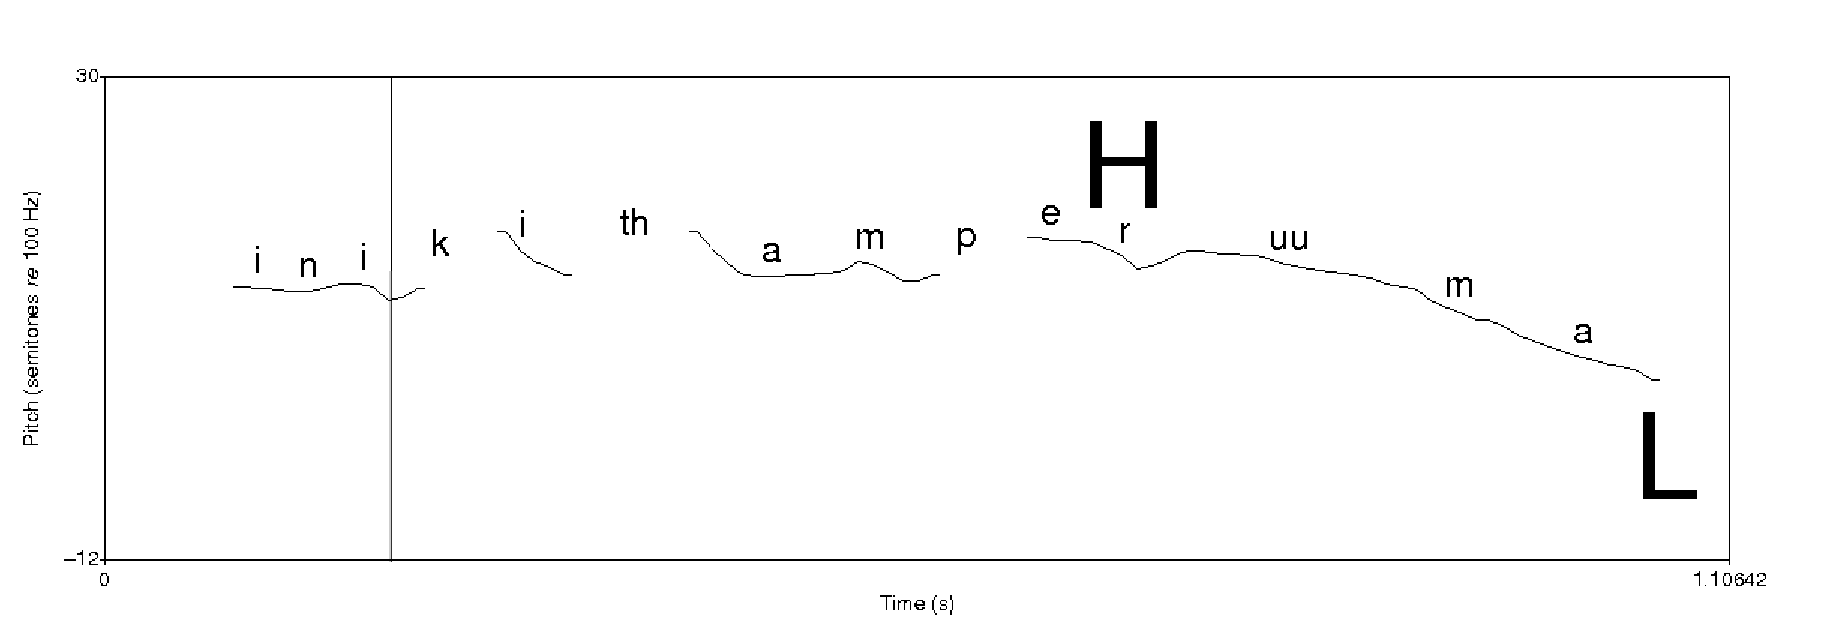
\includegraphics[width=0.5\textwidth]{./pics/kithamperuuma.eps}
\glll    ~   ~         H~~~~L\\
	 ini kitham-pe ruuma \\
     \textsc{prox} \textsc{1pl=poss} house  \\
    `This is our house.'
\z
} \\

In \xref{ex:phon:int:ass:kithamperuuma}, there is no presupposition, only a deictic reference (whose contour we will ignore for now) and an assertion \trs{kithampe ruuma}{our house}. The  assertion receives the HL contour, where H is linked to the beginning of the last lexical word \trs{ruuma}{house}\footnote{The pitch peaks after the k and the th are caused by aspiration and thus artefacts and not part of the intonation proper.} and the L is linked to the end of the utterance.

In \xref{ex:phon:int:ass:kithampenigirisujjadi}, we have a verbal predicate \trs{kitham=pe nigiri su-jaadi}{became our country}. The assertive contour is applied to the predicate with the high tone on the prefix of the last lexical word, the  verb. Then follows a drop to the end of the utterance. The constituents \trs{kaarang}{now}{} and \trs{ini}{\textsc{prox}}{} receive a presuppositive contour, discussed further below.

\xbox{14}{
\ea \label{ex:phon:int:ass:kithampenigirisujjadi}
 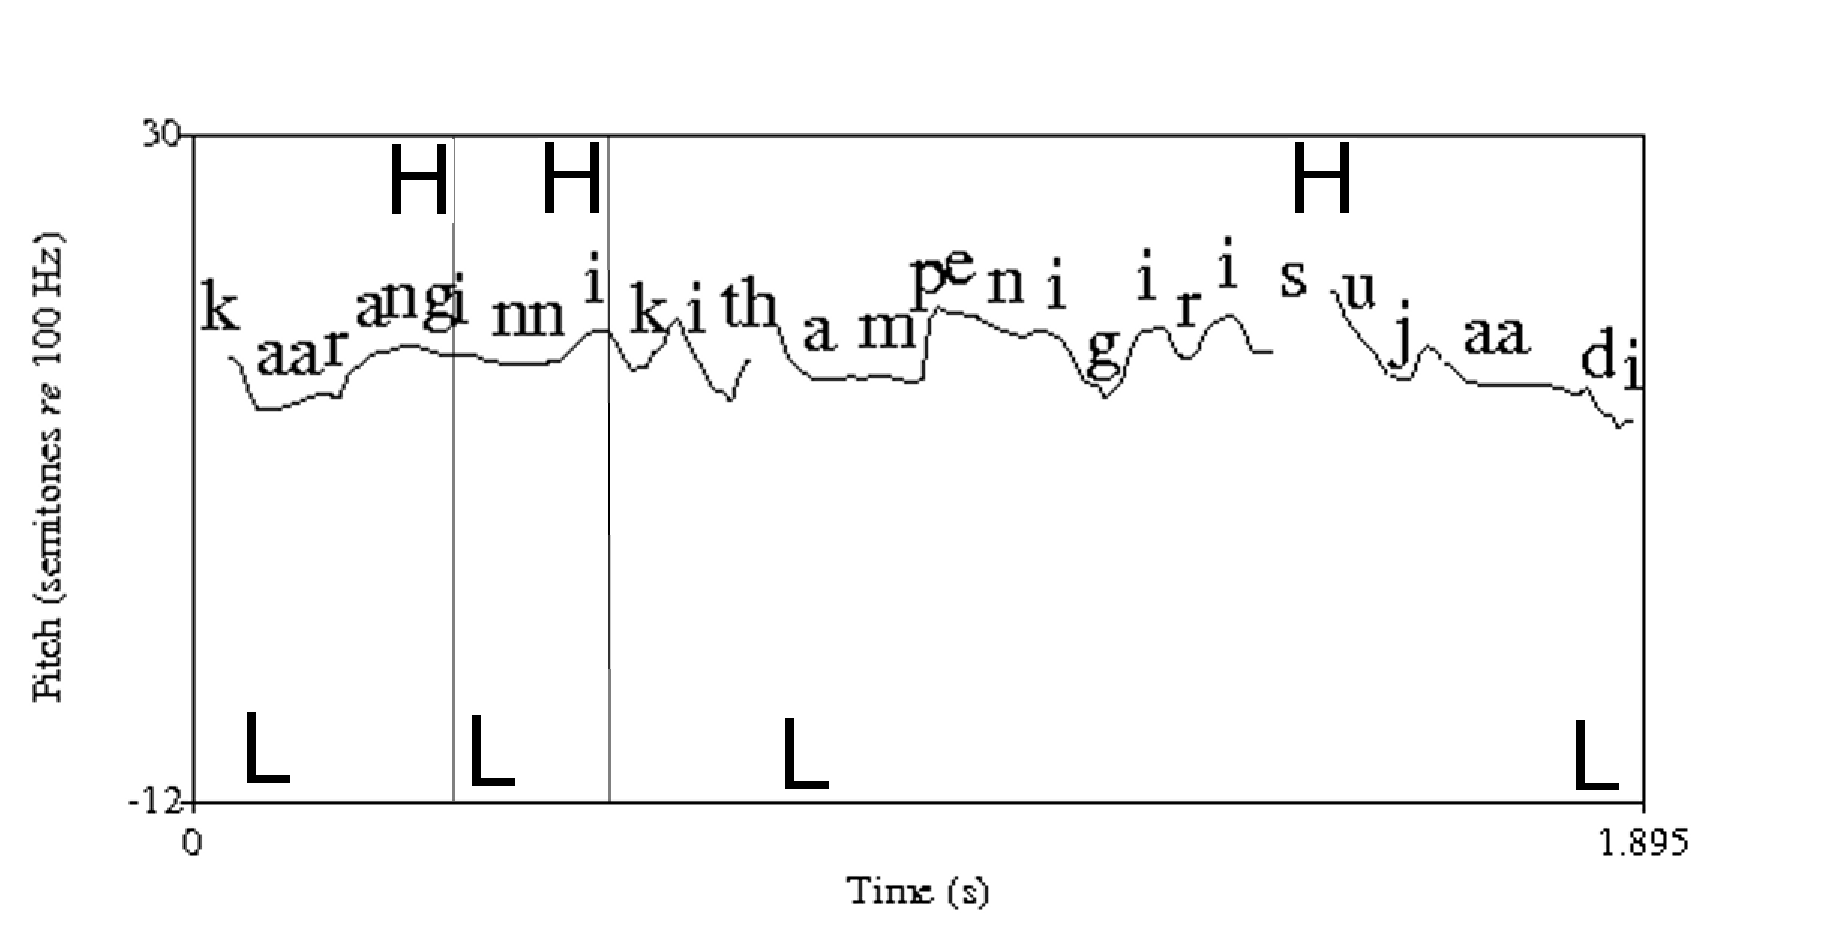
\includegraphics[width=0.5\textwidth]{./pics/newkithampenigiri.eps}
\glll    ~L   	H       ~L         H      ~      ~     H          L\\
	 kaarang $\mid$ inni  $\mid$ kitham=pe nigiri su-jaadi $\mid$\\
     now ~ \textsc{prox} ~ 1\textsc{pl}=\textsc{poss} country \textsc{past}-become \\
    `Now this has become our country.'
\z
} \\

Above we have seen that the last lexical word (noun, verb) receives the high tone of the assertive contour.
In the event that the assertion only contains functional elements, the description formulated above cannot apply. In this case,  the high tone is linked to the last word nevertheless, even if it is not lexical. An example is \trs{kitham}{1pl} in \xref{ex:phon:int:ass:oorampadajo}.

\xbox{14}{
\ea \label{ex:phon:int:ass:oorampadajo}
 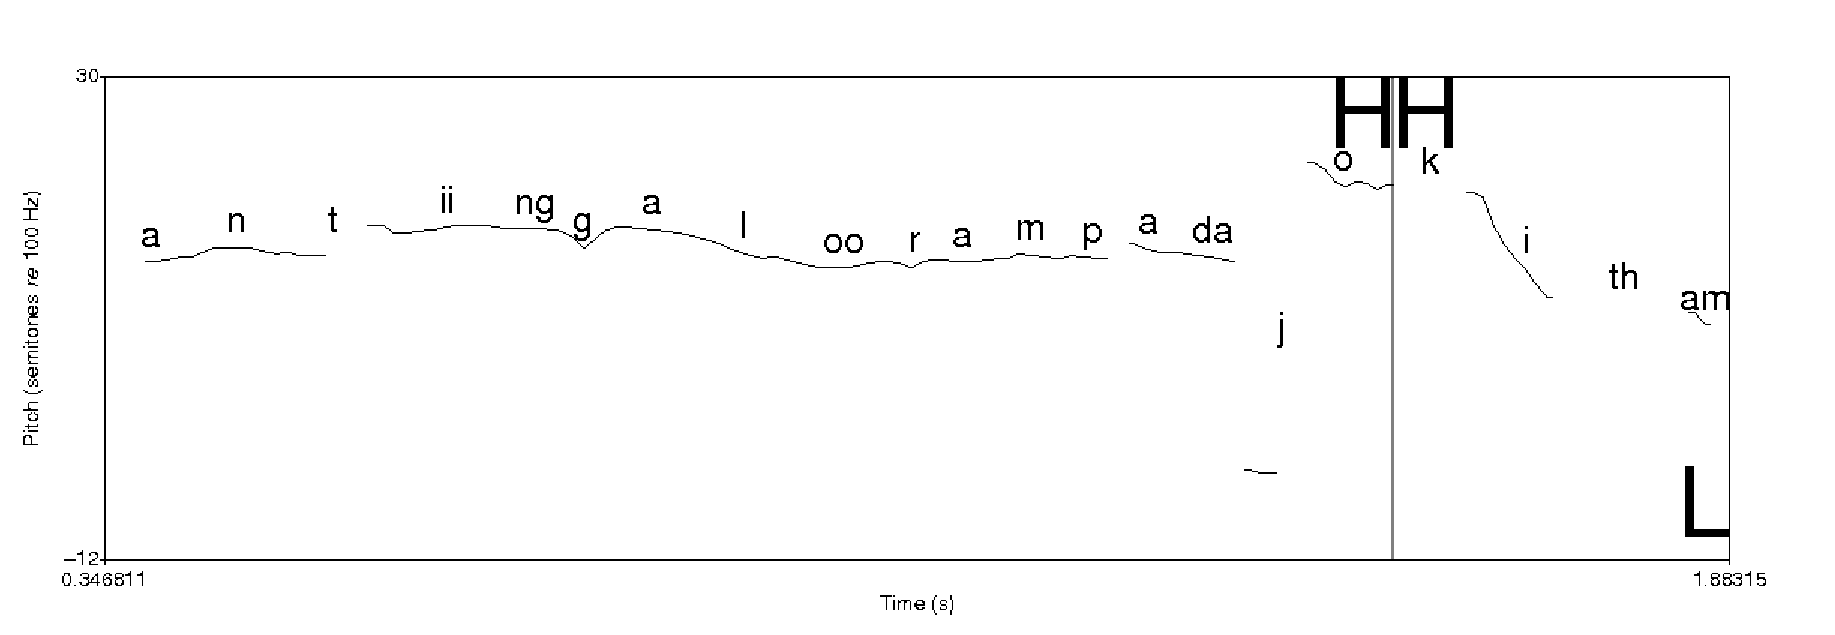
\includegraphics[width=0.5\textwidth]{./pics/oorampadajo.eps}
\glll ~      ~      ~       H       H      L\\
an-tiinggal ooram pada=jo $~\mid~$ kitham $~\mid$\\
 \textsc{past}-settle man \textsc{pl=foc} ~ \textsc{1pl} ~\\
`The people who settled down here are we.'
\z
} \\




In narrow focus, the high tone is linked to the element in focus even if this is not the last lexical element in the assertion. In \xref{ex:phon:int:ass:seelongoorangpada}, the speaker emphasizes the fact that the Malays are no longer East Asians, but Ceylonese. The two presuppositions \trs{kaarang}{now}{} and \trs{kithang}{we}{} are followed by the assertion \trs{SEELON ooram pada}{Ceylon people}. The presuppositions conform to the presuppositive contour, which will be discussed in more detail below. The assertion \em SEELON ooram pada \em receives the assertive HL contour, but H is linked to the emphasized element \em SEELON \em instead of the last lexical element \em ooram\em. This is marked in the graphic by a crossed out H where the normal tone would be expected.


\xbox{14}{
\ea \label{ex:phon:int:ass:seelongoorangpada}
 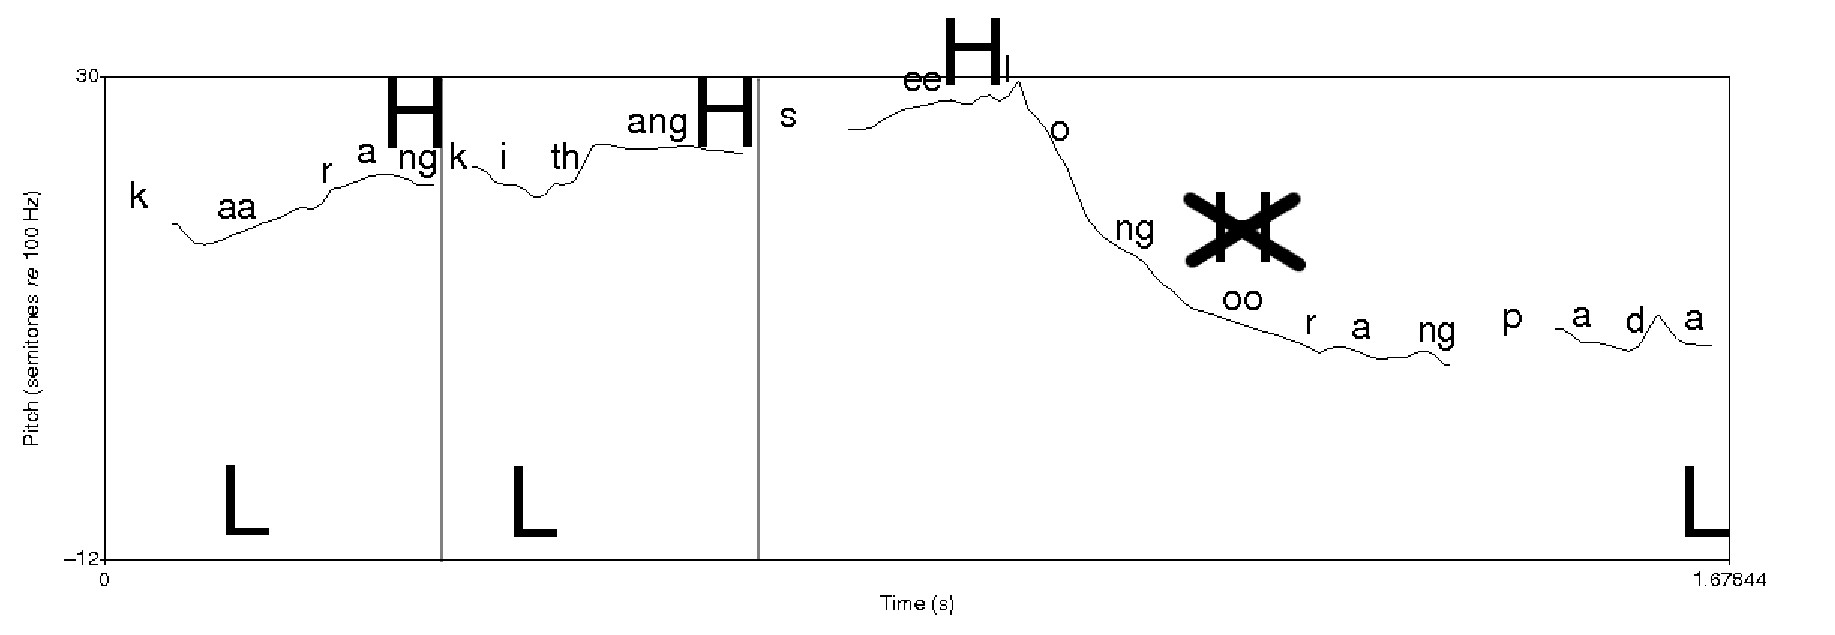
\includegraphics[width=0.5\textwidth]{./pics/seelongoorangpada.eps}
\glll ~~~L      H      ~~L       H      H        ~     ~   L \\
      kaarang $~\mid~$ kithang $~\mid~$ Seelong ooram pada $~\mid$ \\
     now { }   \textsc{1pl} { } Ceylon man \textsc{pl} { } \\
    `Now we are Ceylonese.'
\z
} \\

Imperatives also take the assertive contour, as the following example, taken from cooking instructions, shows. Note that the rice is presupposed and has been talked about earlier, which can be seen from the accusative marker \em =yang\em, which normally only attaches to inanimate referents when they are topical (see Section \ref{sec:morph:=yang}).


\xbox{14}{
\ea \label{ex:phon:int:ass:birrasyanthaaro}
 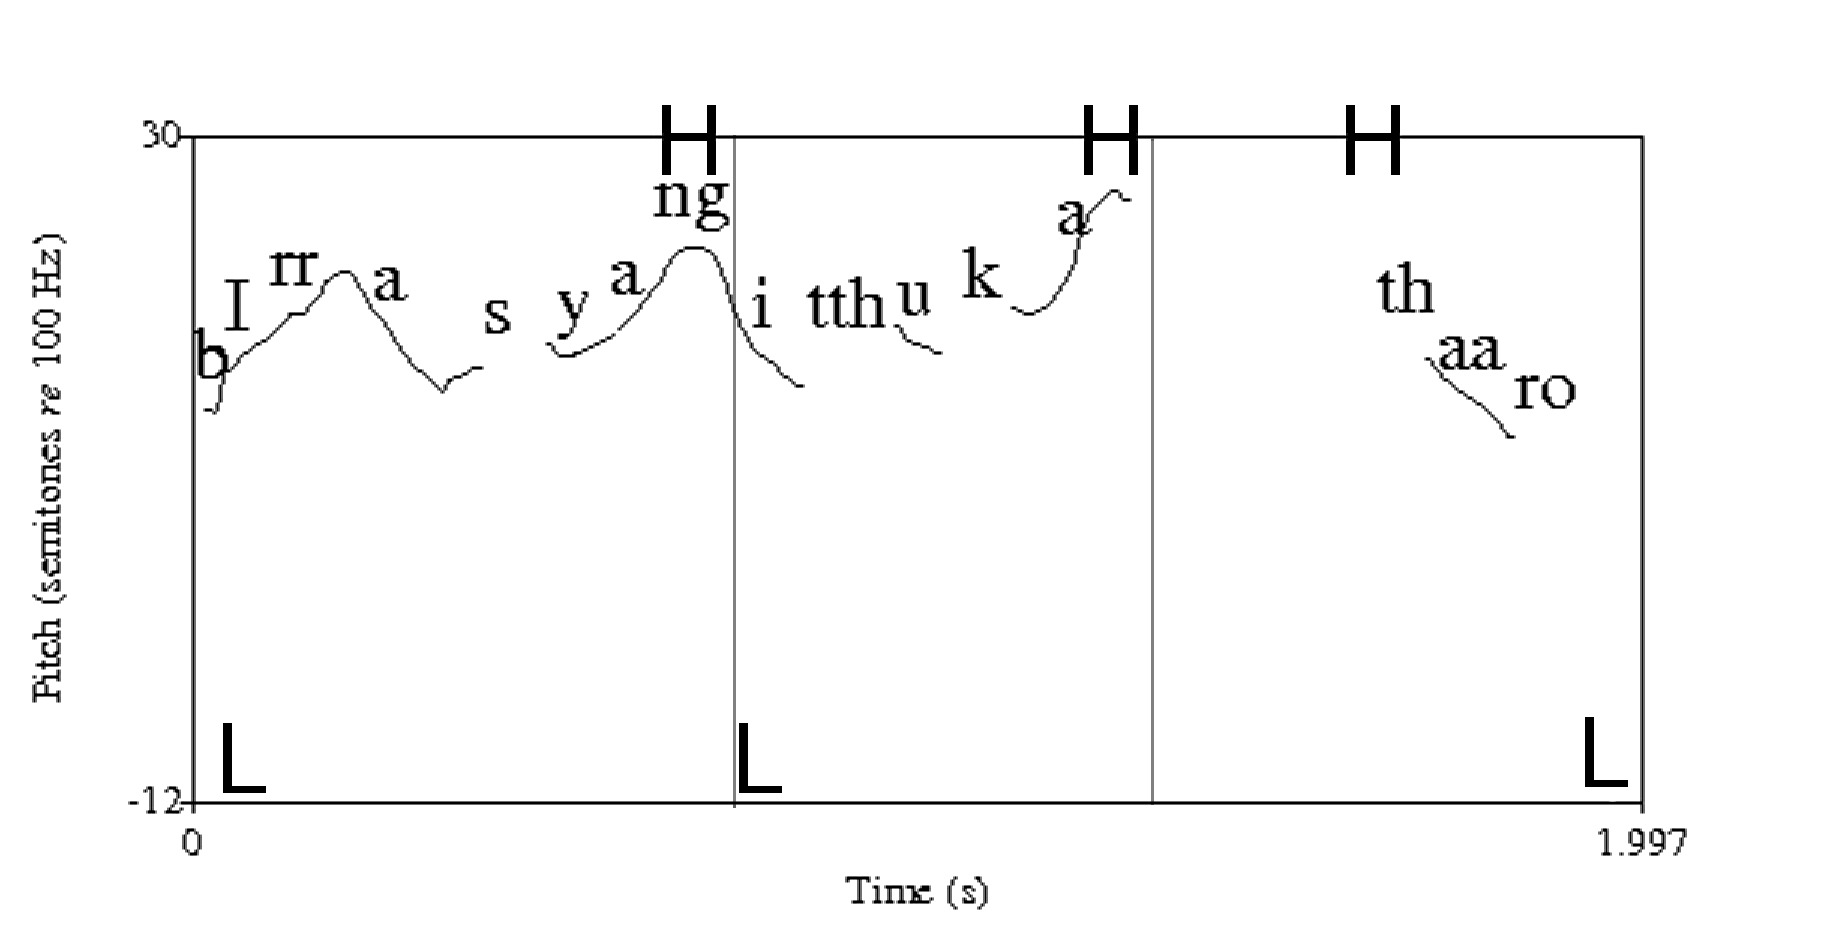
\includegraphics[width=0.5\textwidth]{./pics/birrasyangitthukathaaronew.eps}
\glll ~L             H    ~L       H       ~H       L \\
      bìrras=yang $~\mid$ itthu=ka $~\mid$  thaaro $~\mid$ \\
     raw.rice=\textsc{acc} { } \textsc{dem.dist}=\textsc{loc} { }  put { } \\
    `Add the rice to it!'
\z
} \\

\subsection{Progredient contour}\label{sec:phon:Progredientcontour}
The progredient contour is characterized by a slow steady rise to a high tone at the end. It is used for the non-final elements in a chain of assertions. The enumeration of ethnic groups in \xref{ex:phon:int:ass:cinggalaaada} shows slow rise from start to end of each of the first three phonological phrases, which are progredient. The last phonological phrase has the ``final'' contour, but the intensity decreases so that the graphic cannot represent the very low final pitch. The movement is clear when listening, though.


\xbox{14}{
\ea \label{ex:phon:int:ass:cinggalaaada}
 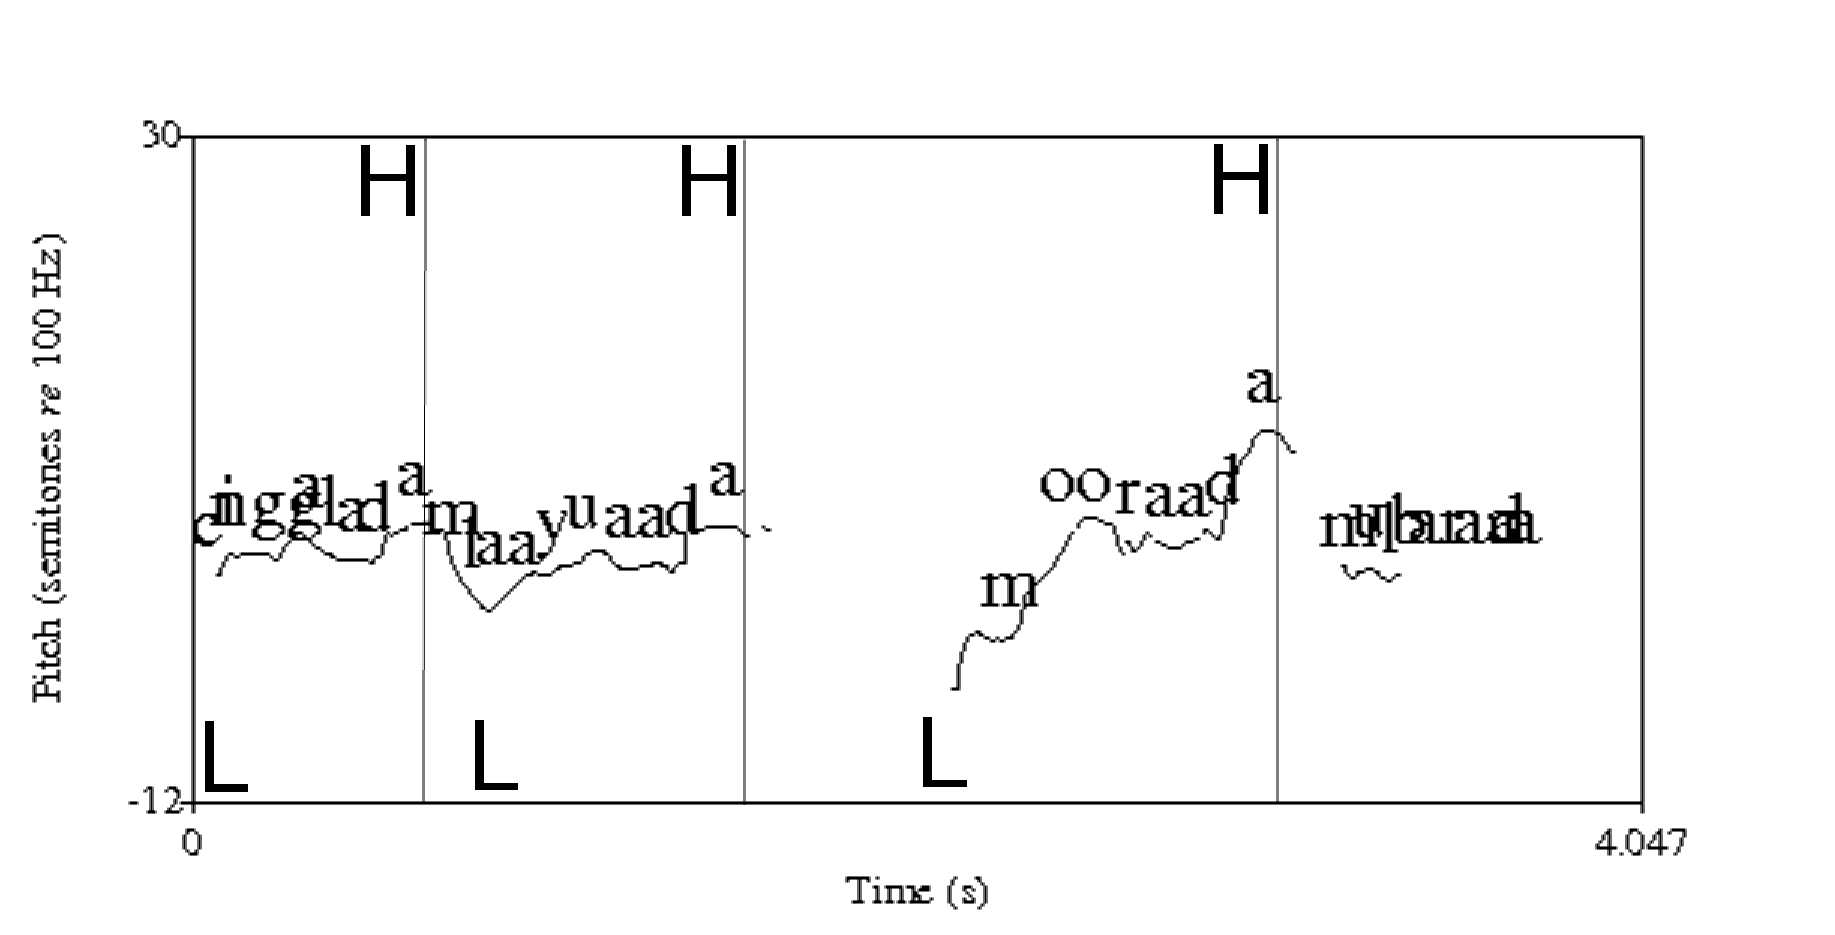
\includegraphics[width=0.5\textwidth]{./pics/cinggalaaadanew.eps}
\glll   L        ~ 	H  	L      ~ 	H  L    ~       H    ~        ~~ (L)\\
	cinggala aada $~\mid~$ 	mlaayu aada $~\mid~$ {\em moor} aada $~\mid~$ 	mùlbar aada $~\mid$\\
        Sinhala exist ~ Malay exist ~ Moor exist ~ Tamil exist ~\\
    `There are Sinhalese, there are Malays, there are Moors, there are Hindus.'
\z
} \\


\subsection{Presuppositive contour}\label{sec:phon:Presuppositivecontour}
The presuppositive contour is characterized by a steady fall to the last syllable and a following steep rise to a high tone target: LH. It is used for presupposed elements, which can be NPs, adjuncts or subordinate clauses.


Subordinate clauses always precede the main clause in SLM and are normally presupposed. Being presupposed, they are realized with a final H tone, normally preceded by a low tone. \xref{ex:phon:int:presup:braambath} illustrates this pattern. The high tone is on the right edge of \trs{kaaving}{marry}, while the low tone is immediately preceding. There is a second presupposition in this utterance \trs{ini mlaayu}{these Malays}. Just like the subordinate clause, this NP receives an LH contour. The assertion has a high tone on the past tense prefix \em su- \em of the last lexical word \trs{braambath}{spread}.


\xbox{18}{
\ea \label{ex:phon:int:presup:braambath}
 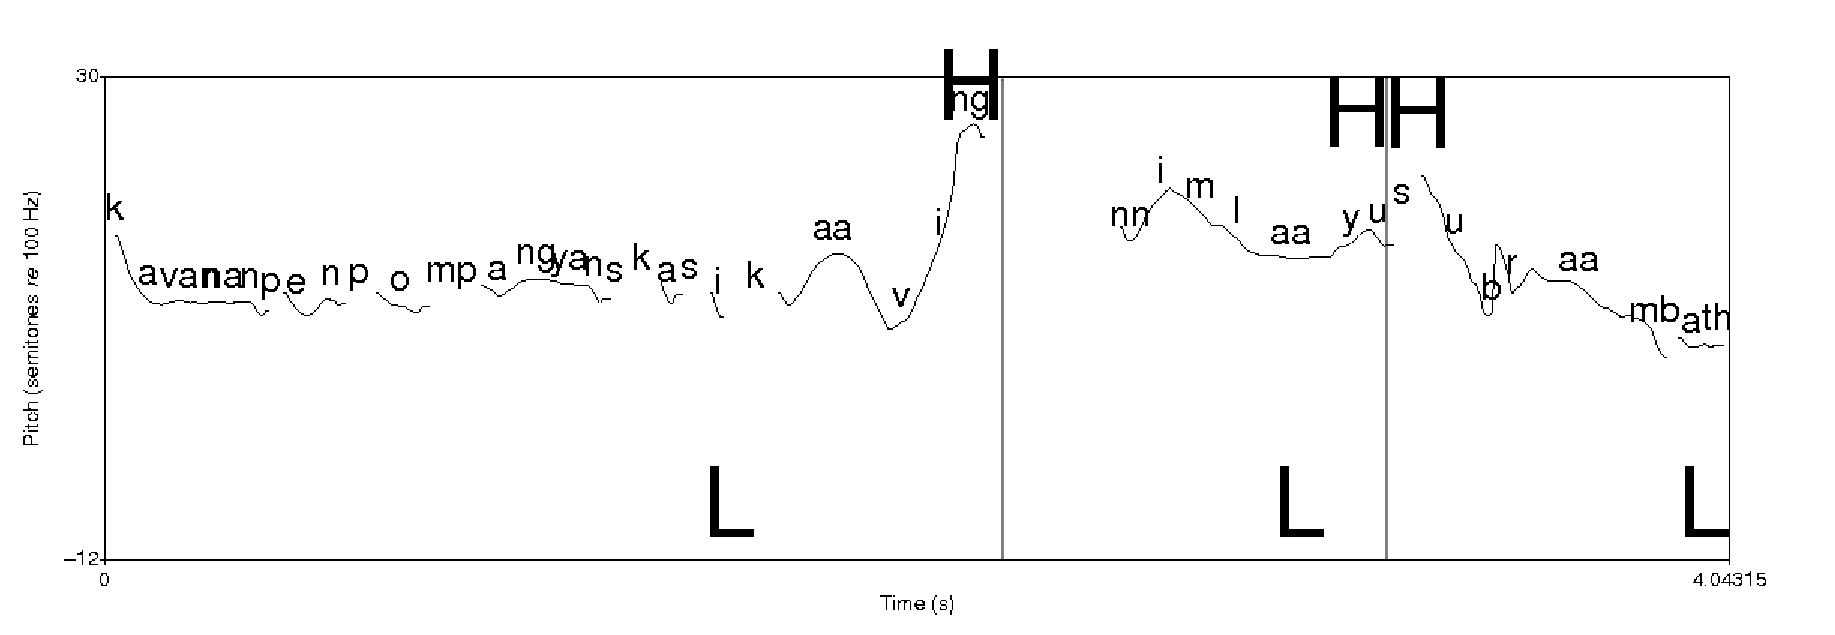
\includegraphics[width=0.5\textwidth]{./pics/braambath.eps}
\glll     ~    ~            ~         ~       ~~L     H          ~ ~~~L      H      H           L\\
	 ini kavanan=pe prompang=yang as-kasi kaaving $~\mid~$ nni mlaayu $~\mid~$ su-braa\u mbath $~\mid$\\
     \textsc{prox} group=\textsc{poss} female=\textsc{acc} \textsc{cp}-give marry ~ \textsc{prox} Malay ~ \textsc{past}-spread ~ \\
    `Having married their daughters, these Malays spread.' 
\z
} \\



In \xref{ex:phon:int:presup:blaajar}, there are two presupposed elements, and one assertion. The presupposed elements are \trs{kithampe aanak pada=jo}{our children}{} and \trs{skaarang}{now}. These receive a low tone on the nucleus of the last syllable (excluding the clitic \em =jo\em) and a high final tone. The assertion \trs{baenang cinggala sablaajar}{learnt Sinhala well}{} receives a high tone on the prefix of the last lexical word \trs{blaajar}{learn} and a low tone target assigned at the end.

\xbox{15}{
\ea \label{ex:phon:int:presup:blaajar}
 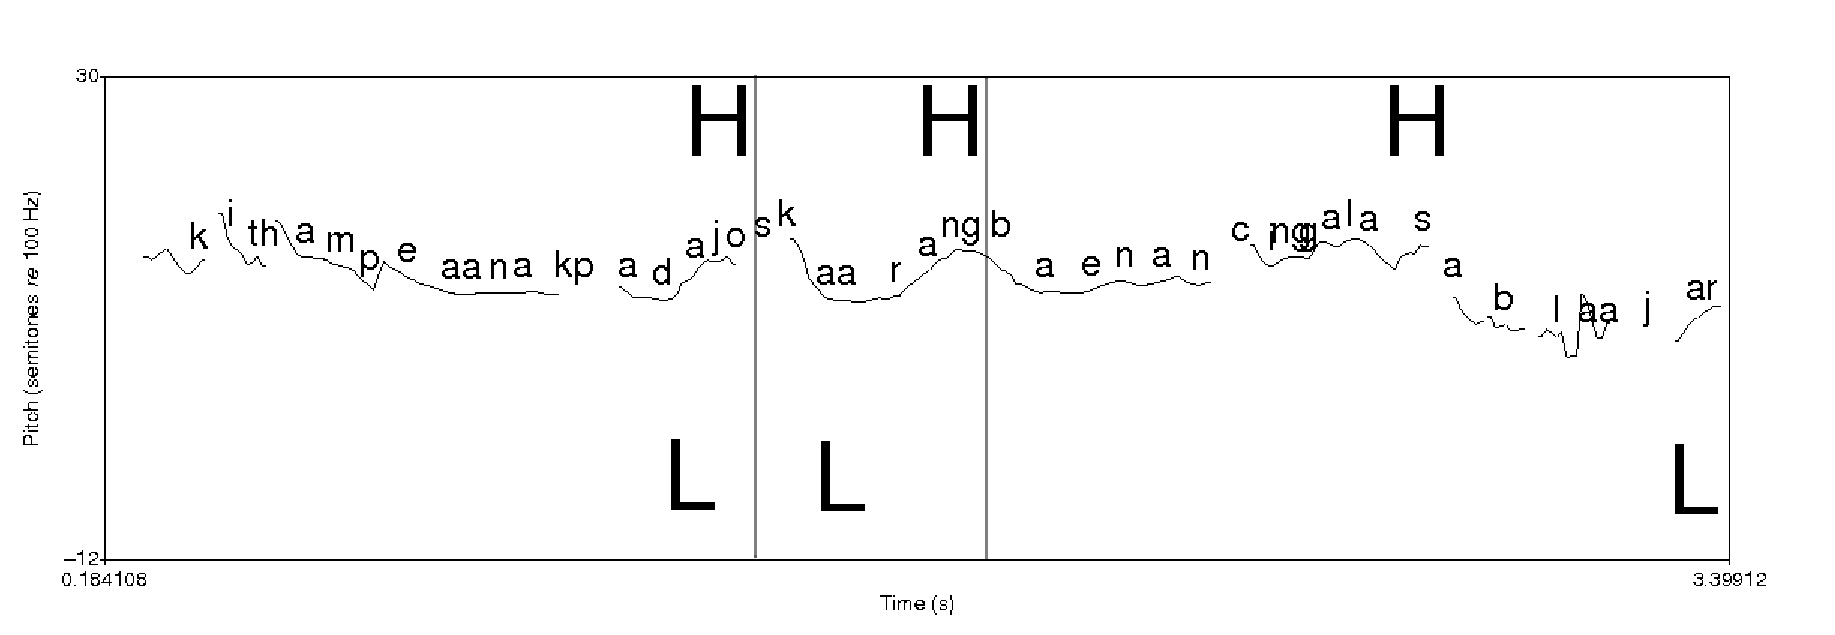
\includegraphics[width=0.5\textwidth]{./pics/blaajar.eps}
\glll ~      ~    ~~~~~L H  ~~~~L	 H  ~       ~       H L\\
 kitham=pe aanak pada=jo $~\mid~$ skaarang $~\mid~$ bae=na cinggala sa-blaajar $~\mid$\\
 \textsc{1pl=poss} child \textsc{pl}=\textsc{emph} ~ now ~ good=\textsc{dat} Sinhala \textsc{past}-learn ~\\
`Our children have learnt Sinhala well.'
\z
} \\

Things are similar in \xref{ex:phon:int:presup:laskallitherapi}, where the presupposed constituents \trs{laskalli}{again}{} and \trs{kithampe nigirinang}{to our country} receive a LH tone at the right edge. The assertion \trs{thàràpii}{did not go} receives high tone on the prefix of the last lexical element and a low final tone.

\xbox{14}{
\ea \label{ex:phon:int:presup:laskallitherapi}
 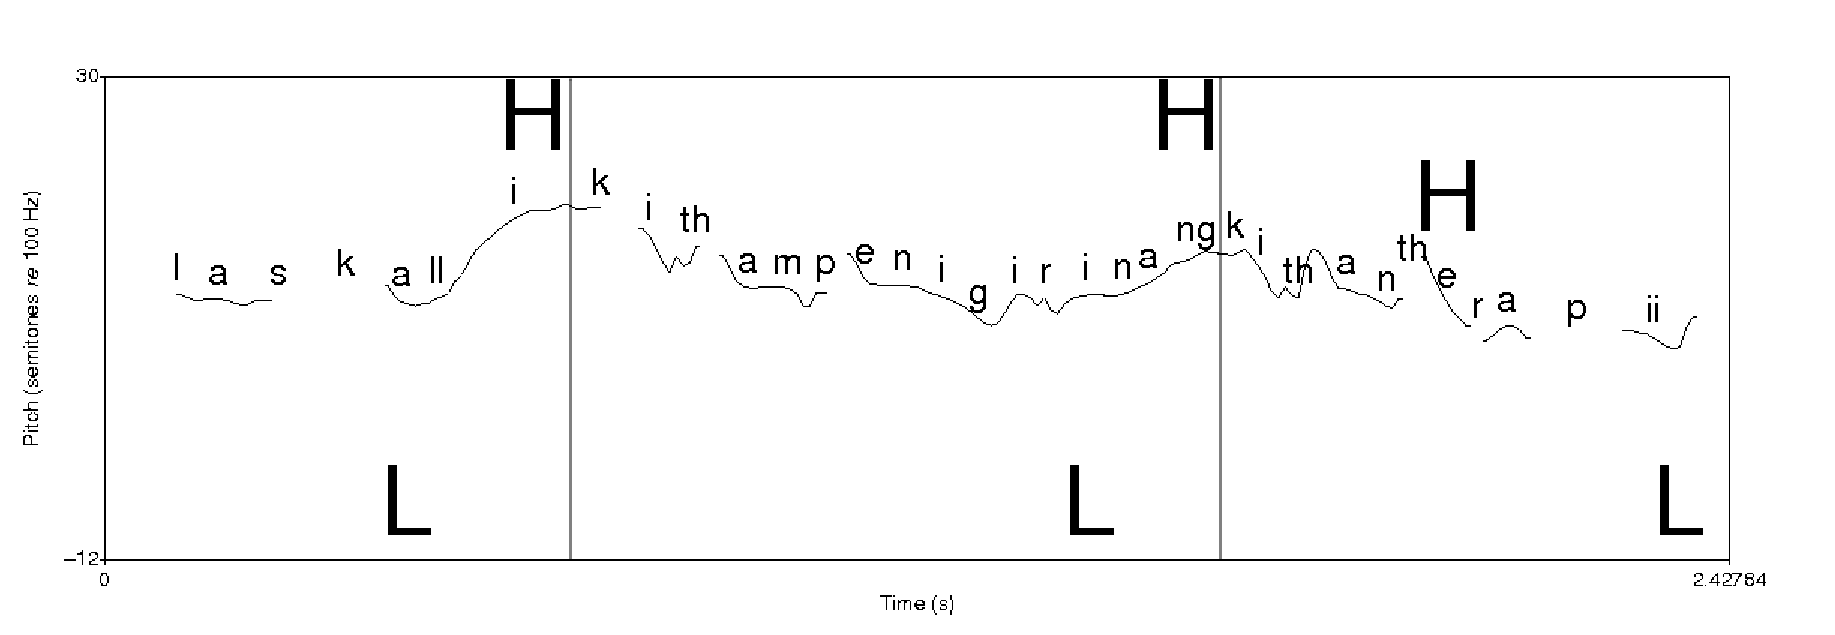
\includegraphics[width=0.5\textwidth]{./pics/laskallitherapi.eps}
\glll ~~~~L     H          ~     ~~~~~~L       H     ~      ~~~H        L  \\
      laskalli $~\mid~$  kitham=pe nigiri=nang $~\mid~$ kithang thàrà-pii $~\mid$ \\
      again ~ \textsc{1pl=poss} country=\textsc{dat} ~ \textsc{1pl} \textsc{neg.past}-go ~ \\
    `We did not go back to our country.' 
\z
} \\



\xref{ex:phon:int:presup:ciinggal} shows a more complex sentence. The presupposed constituent \trs{andaathang ooram pada}{the men who had come} receives a LH tone on the right edge. So do the subordinates \trs{spìrrang}{having waged war} and \trs{deranna asbanthu}{having helped him}. The predicate \trs{siinijo suciinggal}{settled down right here} receives a high tone on the  prefix of last lexical element \trs{ciinggal}{settle} and a low final tone.


\xbox{18}{
\ea \label{ex:phon:int:presup:ciinggal}
 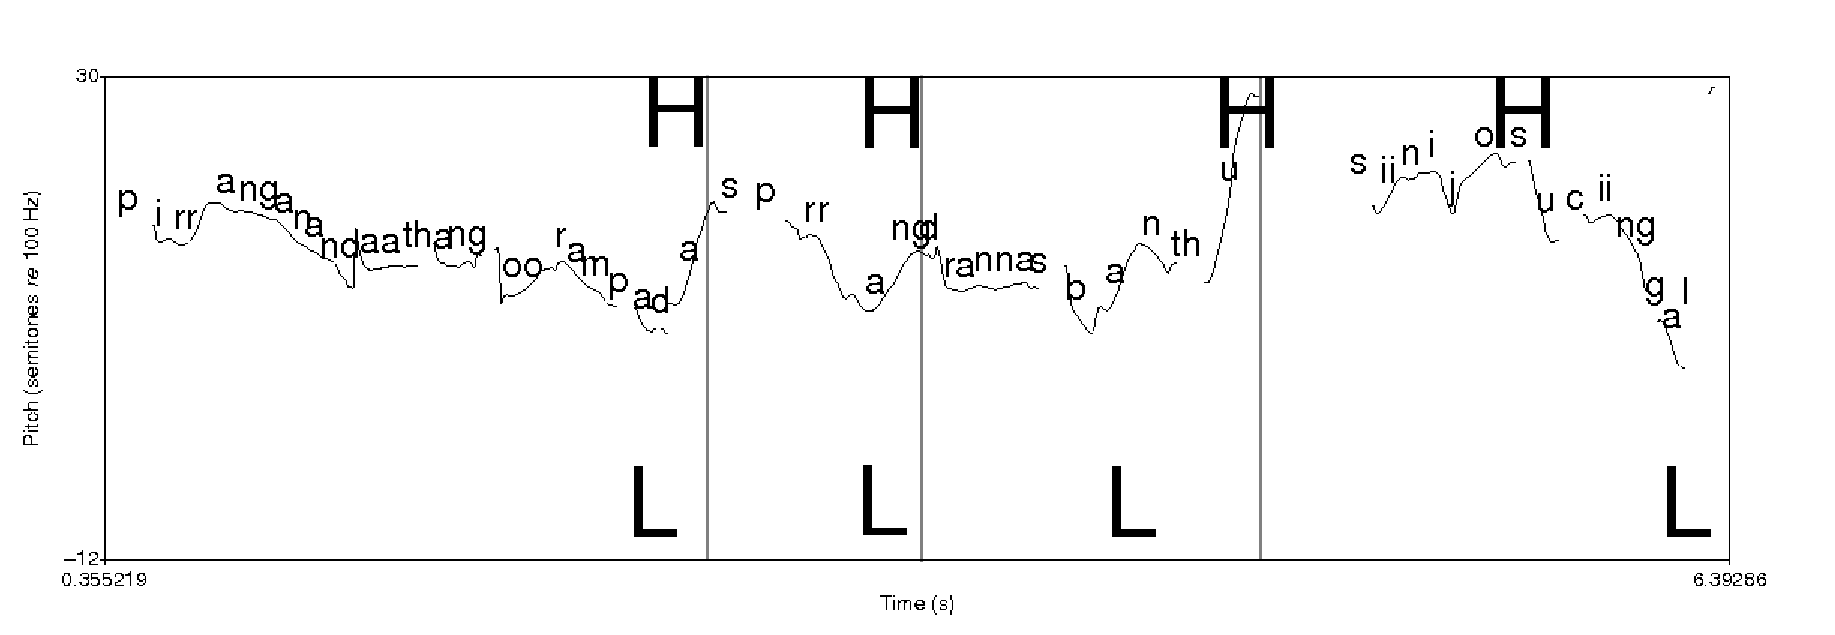
\includegraphics[width=0.5\textwidth]{./pics/ciinggal.eps}
\glll 	~ ~	~	~~L	H	~~~~~~~L	H	~	  ~~~~~~L 	H	~	H 		L\\
       pìirang=na an-daathang ooram pada $~\mid~$ s-pìrrang $~\mid~$  deran=na as-banthu $~\mid~$  siini=jo su-cii\u n\u ggal $~\mid$ \\
      war=\textsc{dat} \textsc{past}-come man \textsc{pl} ~ \textsc{cp}-wage.war ~ 3=\textsc{dat} \textsc{cp}-help ~ here=\textsc{emph} \textsc{past}-settle  \\
    `The men who had come, after having waged war and helped him, settled down.' 
\z
} \\

% The final example of this section shows layering of two contours in the first part, where we find a subordinate clause with a presuppositive contour, embedded in which there are again smaller presuppositive contours. The  pitch movement corresponds to the syntactic importance of the break. The first two movements are inside the subordinate clause and are less important, but the final movement is very steep.
% 
% \xbox{18}{
% \ea \label{ex:phon:int:presup:baaenanmgoornegnamblaakanginisanthangyangitthunamthuuvang}
%  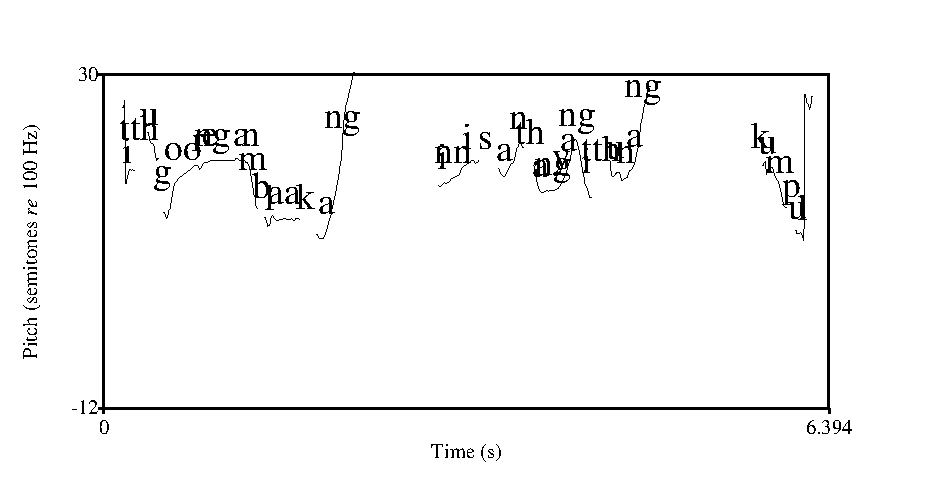
\includegraphics[width=0.8\textwidth]{./pics/itthugoorengnamblaakangnew.eps.eps}
% \glll L            H      L             H        L           H           ~~L        ~        H         L          H        H        L\\
%       itthu $~\mid~$  gooreng=nam $~\mid~$   blaakang $~\mid\mid~$   ini santhang=yang $~\mid~$   itthu=nam $~\mid~$   kumpul $~\mid~$  \\
%       good=\textsc{dat} ~ \textsc{inf}-fry=\textsc{dat} ~ after ~ \textsc{prox}    coconut.milk=\textsc{acc} ~  \textsc{dist=dat}  ~ pour\\
%     `After frying well, add the coconut milk to it.'
% \z
% } \\
% 




% see Stoel 2005


% Negative assertions have a similar contour \xref{ex:phon:int:ass:bissaratthukumpulan}. The pitch fall starts at the \em ku- \em of kumpulan.
% 
% \xbox{14}{
% \ea \label{ex:phon:int:ass:bissaratthukumpulan}
%  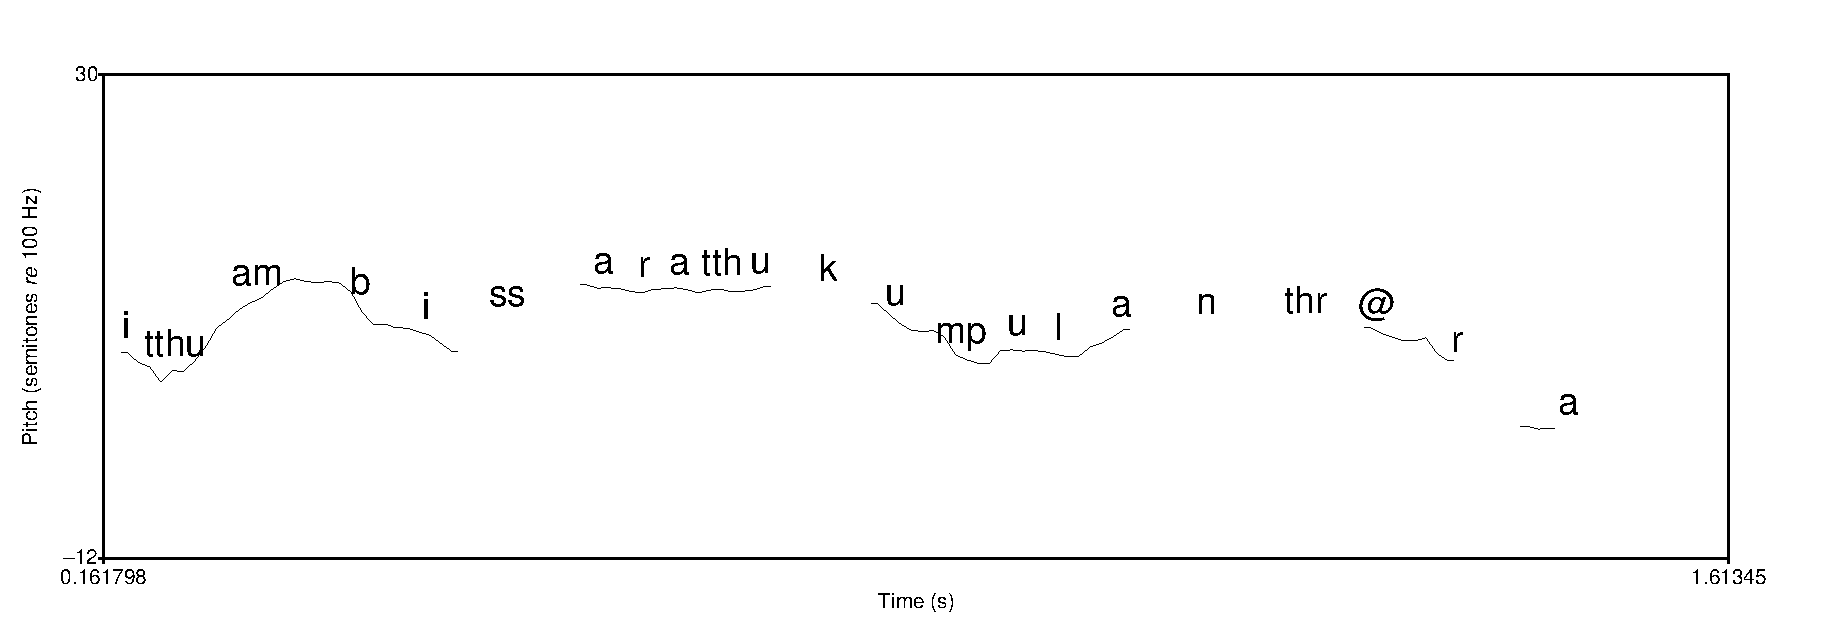
\includegraphics[width=0.5\textwidth]{./pics/neg.eps}
% \gll itthunam, bìssar atthu kumpulan th\E raa \\
%      therefore big \textsc{indef} association \textsc{neg}  \\
%     `Therefore, there are no big associations.'
% \z
% } \\



% \xbox{14}{
% \ea\label{ex:phon:int:ass:luppasthaangang}
%  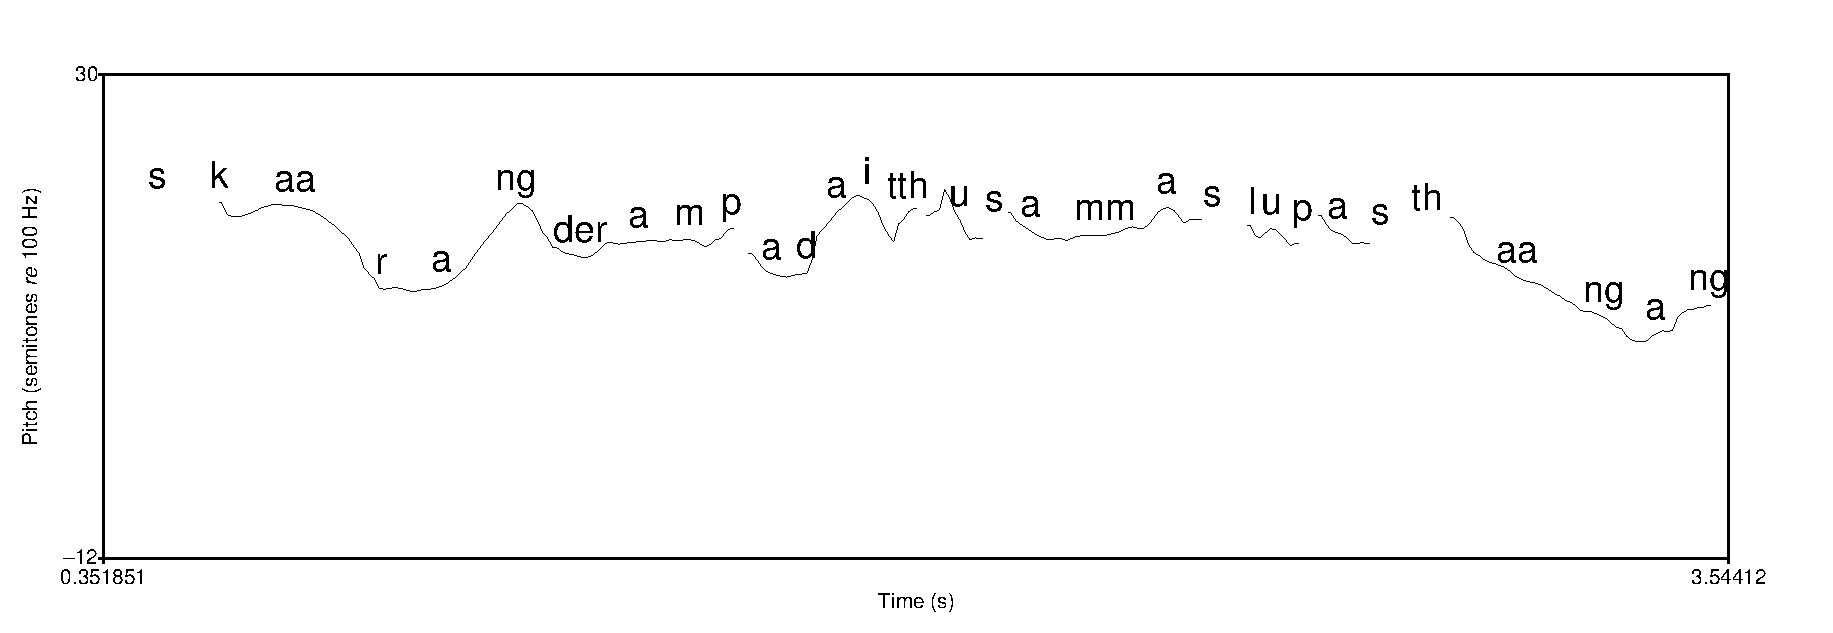
\includegraphics[width=0.5\textwidth]{./pics/luppasthaangang.eps}
% \gll skaarang dheram pada itthu samma as-luppas thaangang \\
%      now \textsc{3pl} \textsc{pl} \textsc{dist} all \textsc{cp}-leave hand  \\
%     `Now they left it all behind.'
% \z
% } \\






\subsection{Question contour}\label{sec:phon:Questioncontour}
The question contour is identical to the presuppositive contour: LH on the last syllable. It might be possible to combine them into a ``non-assertive'' contour; for expository reasons this is not done here. The question contour is used for interrogative illocution. Given that there is also segmental material which signals questions (WH-words or the clitic \em =si\em), the question contour is not obligatory if either of these are present.

Example  \xref{ex:phon:int:q:aapeyang} shows the question contour on a WH-question introduced by \trs{aapeyang}{what}. The pitch rises to the right edge from an immediately preceding low tone linked to \trs{kijja}{do}. The preceding NP \trs{dram pada}{they}{} and the preceding subordinate \trs{deram pada lae atthu pukuran mà-gijja thàrboole subbath}{Since they could not do other work}{} have the presuppositive contour, which is emically identical to the question contour. All three contours in this utterance have a final high  tone, and a preceding low tone, although the latter cannot be located exactly in the subordinate clause.


\xbox{12.5}{
\ea \label{ex:phon:int:q:aapeyang}
 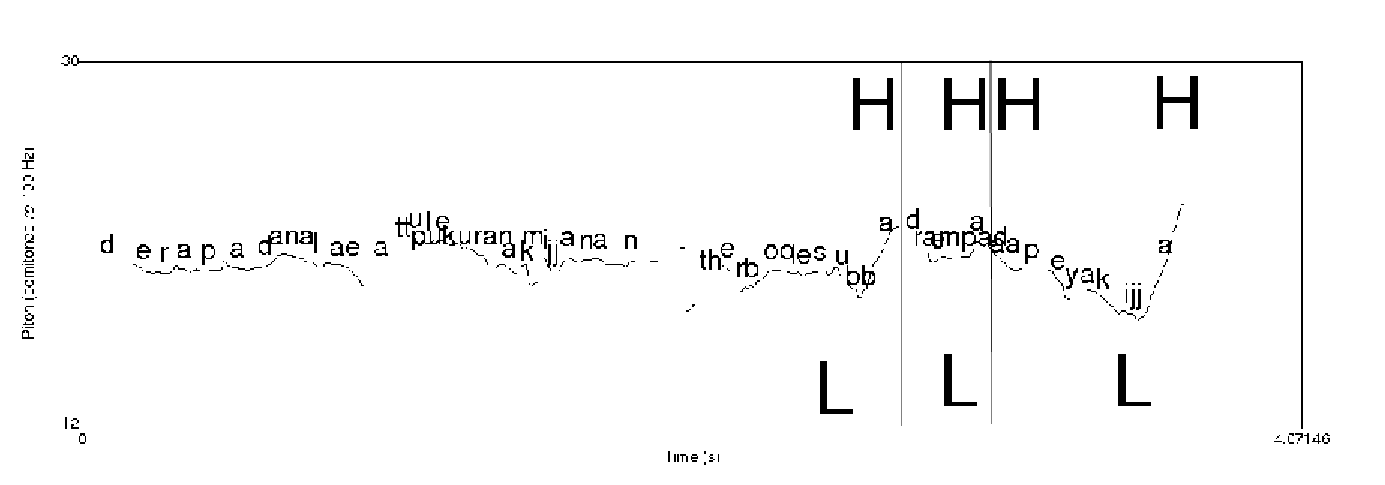
\includegraphics[width=0.5\textwidth]{./pics/aapeyang.eps}
\glll      ~    ~    ~    ~     ~      ~        ~        ~~L?         H      ~    ~~L   H       H         ~~~~~~L    H  \\
	 deram pada lae atthu pukuran mà-gijja thàrboole subbath $~\mid~$ dram pada $~\mid~$ aape=yang eng-kijja? $~\mid~$ \\
      \textsc{3pl} \textsc{pl} other \textsc{indef} work \textsc{inf}-make cannot because ~ \textsc{3pl} \textsc{pl} ~ what=\textsc{acc} \textsc{past}-do \\
    `Since they could not do other work, what did they do?' 
\z
} \\

YN-questions without the clitic \em =si \em also have the question contour, as in \xref{ex:phon:int:q:netherlandka}

\xbox{14}{
\ea \label{ex:phon:int:q:netherlandka}
 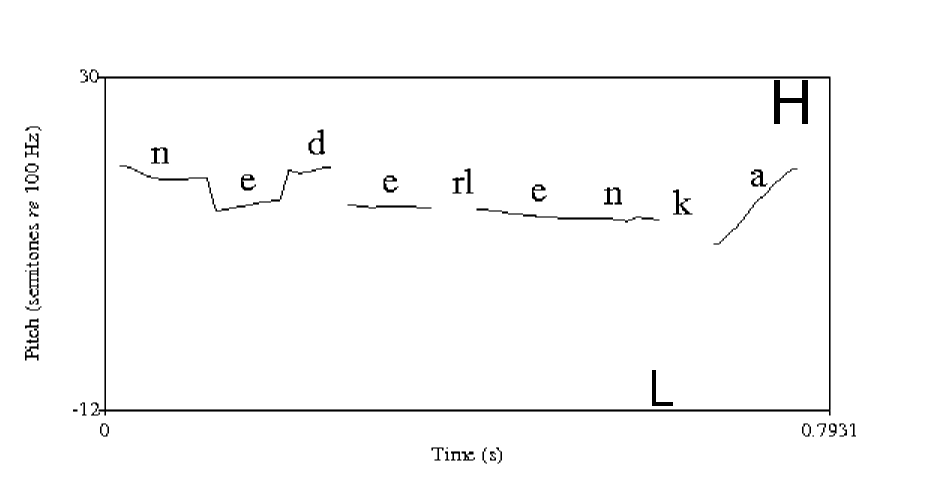
\includegraphics[width=0.5\textwidth]{./pics/nederlenkanewHL.eps}
\glll       ~  ~~~~~~~~~~~~~~~L       H \\
	{ } {\em Netherland}-ka $\mid$ \\
     {} Netherlands-\textsc{loc}  \\
    `Do they live in the Netherlands?' 
\z
}


Another example is \xref{ex:phon:int:q:gheena}, where the speakers ask a younger speaker for the word for `ghee'. The pitch rises steadily to the end of the question.


\xbox{14}{
\ea \label{ex:phon:int:q:gheena}
 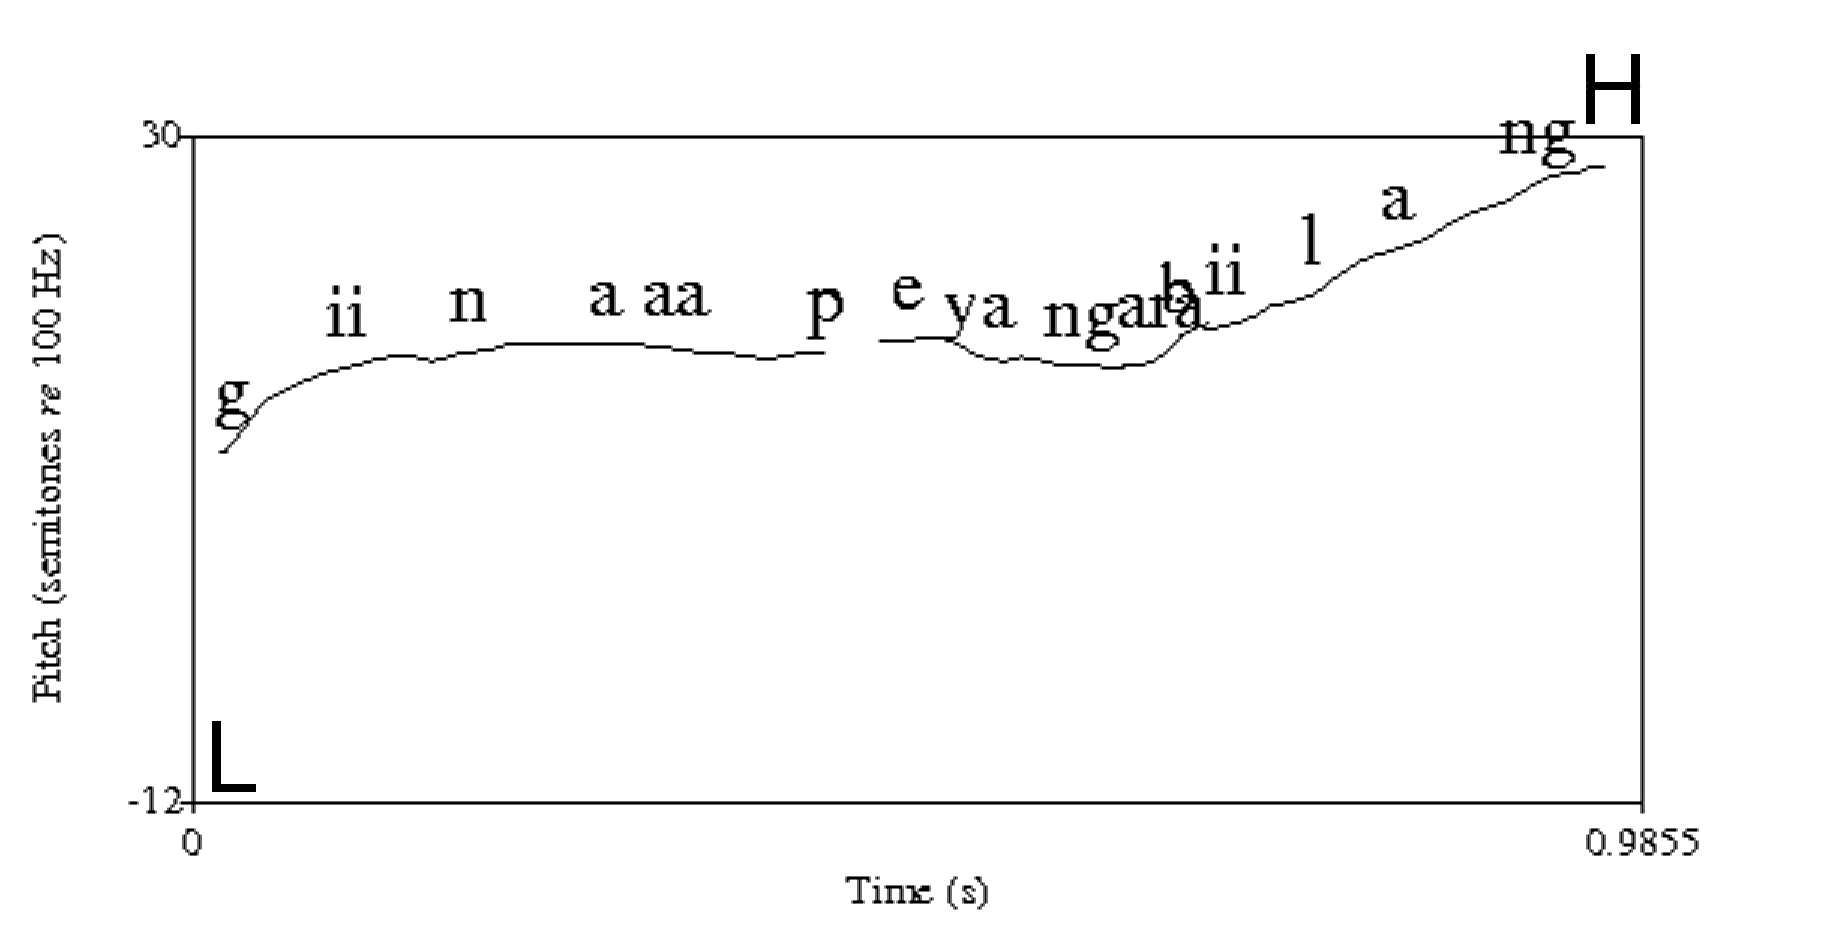
\includegraphics[width=0.5\textwidth]{./pics/gheenaaapeyangarabiilangnew.eps}
\glll       ~L  		~  ~     ~        H \\
	{\em ghee} =na aapeyang biilang $\mid$ \\
    { } =\textsc{dat} what say \\
    `How do you say for ``Ghee''?'
\z
}



When the interrogative clitic \em =si \em is present, the question contour can be present as in \xref{ex:phon:int:q:sudaarasudaari} or absent, as in \xref{ex:phon:int:q:puaasamuusing}. This seems to correlate with question type. In \xref{ex:phon:int:q:sudaarasudaari}, the speaker requests information about the existence of siblings, whereas in \xref{ex:phon:int:q:puaasamuusing} the speaker requests confirmation of her assumption that the addressee was not in Sri Lanka during the fasting period. Request for information is signalled both segmentally and suprasegmentally in \xref{ex:phon:int:q:sudaarasudaari}, while request for confirmation is only marked segmentally in \xref{ex:phon:int:q:puaasamuusing}, and not suprasegmentally.


\xbox{14}{
\ea \label{ex:phon:int:q:sudaarasudaari}
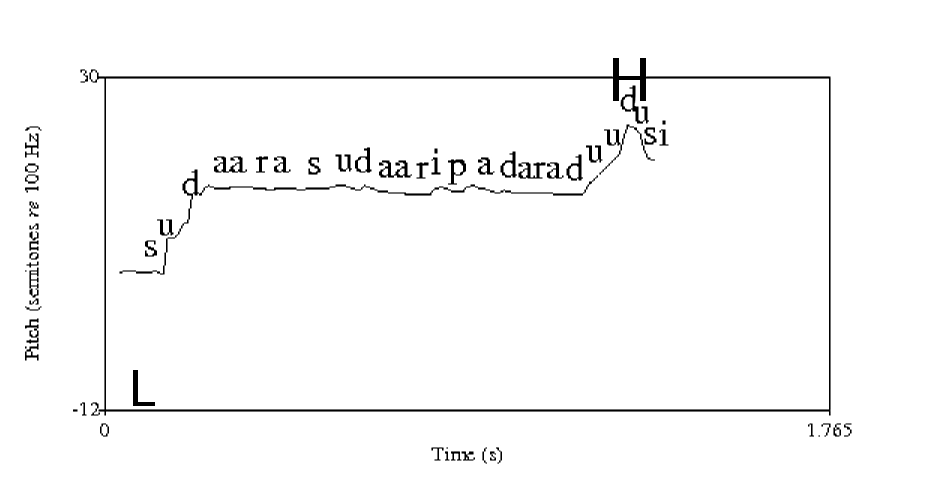
\includegraphics[width=0.5\textwidth]{./pics/sudaarasudaaripadanewHL.eps}
\glll ~L          ~        ~        ~~~~~~~~~~~~~H   \\
      sudaara sudaari pada arà-duuduk=si \\
      brothers sisters \textsc{pl} \textsc{non.past}-be=\textsc{interr}  \\
    `Do you have brothers or sisters?' 
\z
} \\


\xbox{14}{
\ea\label{ex:phon:int:q:puaasamuusing}
 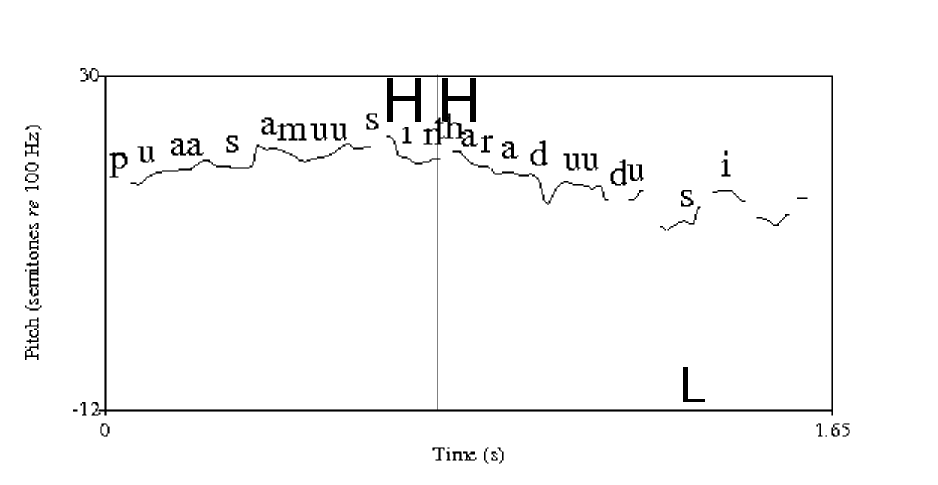
\includegraphics[width=0.5\textwidth]{./pics/puaasamuusing1newHL.eps}
\glll  ~      ~~~~~H	H~~~~~~~~~~~~L\\
       puaasa muusing thàrà-duuduk=si  \\
     fasting period \textsc{neg.past}-live=\textsc{interr}  \\
    `You were not here during the fasting period, were you?' 
\z
} \\


\subsection{Case study}\label{sec:phon:Casestudy}
The intonational patterns for assertions, questions and commands will be exemplified by a short conversation recorded in Badulla on  January 15, 2006. After some linguistic production stimulated by the researcher, the speakers have a little rest and chat about his family.  The existence of the recording device is forgotten. This fragment was chosen because of the naturalistic setting and because various concise speech acts with distinct intonation contours follow each other in short sequence.
Especially interesting are the different functions that interrogatives can have. They can be used to request information, or to request confirmation. This corresponds to different intonatory contours and to the presence or absence of the interrogative clitic \em =si.\em

%  B060115cvs03.trs


\begin{tabular}{lp{4cm}}\hspace{-1cm}
\xbox{12}{
\ea
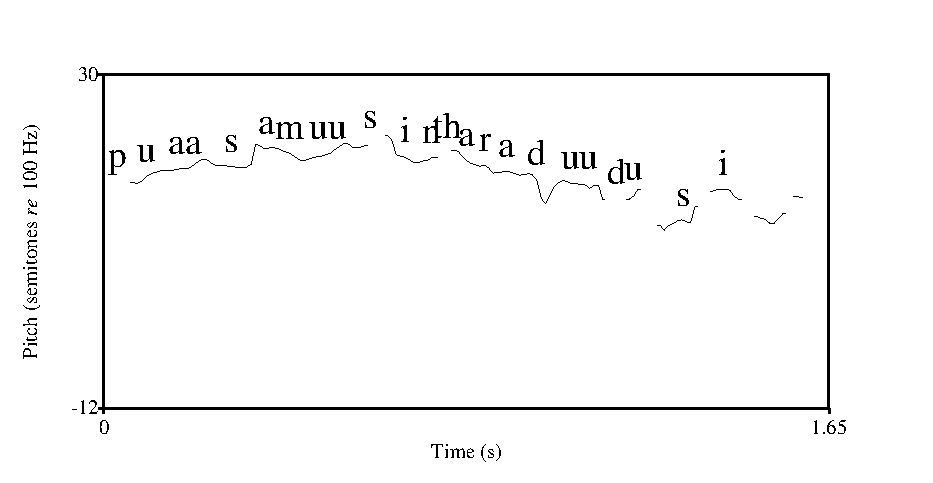
\includegraphics[width=0.5\textwidth]{./pics/puaasamuusing1new.eps}
\glll  ~     ~~~~H  ~ 		H 		L\\
     puaasa  muusing $\mid$ thàrà-duuduk=si $\mid$ \\
     fasting period ~ \textsc{neg.past}-live=\textsc{interr}  \\
    `You were not here during the fasting period, were you?' 
\z
} 
&\vspace{1cm}
 
 \textbf{Comment}: The negated predicate \trs{thàràduuduk}{were.not} together with \em =si \em indicate a presumption of absence, whose correctness is requested to be confirmed. The intonation contour is HL, like an assertion.\\
\end{tabular}


\begin{tabular}{lp{4cm}}\hspace{-1cm}
\xbox{12}{
\ea
 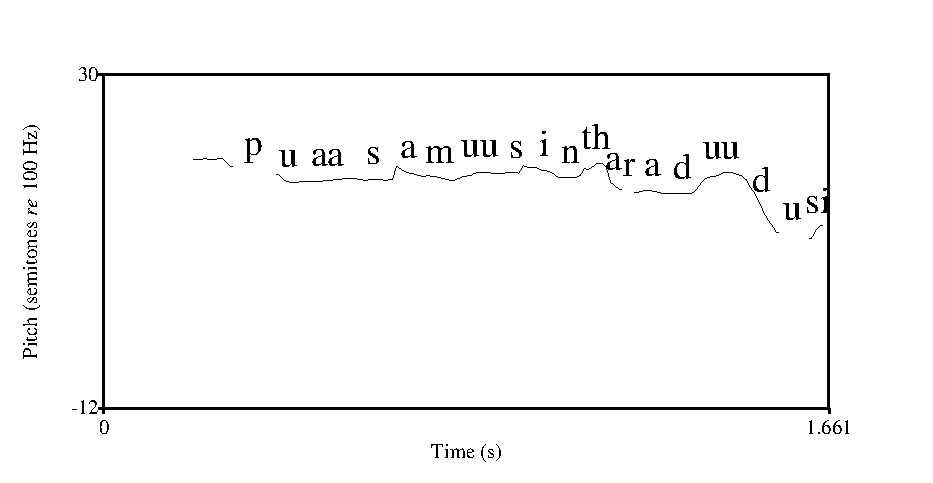
\includegraphics[width=0.5\textwidth]{./pics/puaasamuusing2new.eps}
\glll  ~     ~~~  ~ ~~~~~~~~~~H 		L\\
     puaasa muusing $\mid$ thàrà-duuduk=si $\mid$  \\
     fasting period ~ \textsc{neg.past}-live=\textsc{interr}  \\
    `You were not here during the fasting period, were you?'
\z
}
&\vspace{1cm}
 
 \textbf{Comment}: as above\\
\end{tabular}


\begin{tabular}{lp{4cm}}\hspace{-1cm}
\xbox{12}{
\ea
 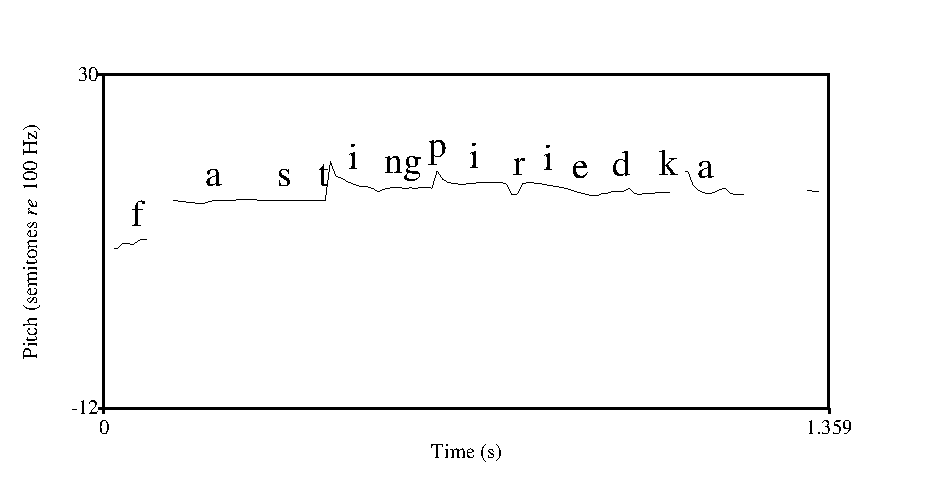
\includegraphics[width=0.5\textwidth]{./pics/fastingperiodkanew.eps}
\glll ~ ~ H\\
     {\em fasting} {\em period}=ka $\mid$ \\
     fasting period=\textsc{loc}  \\
    `In the fasting period' 
\z
}
&\vspace{1cm}
 
 \textbf{Comment}: an elaboration of the preceding question. Very slight rising intonation, since it is not a completely new question.\\
\end{tabular}



\begin{tabular}{lp{4cm}}\hspace{-1cm}
\xbox{12}{
\ea
 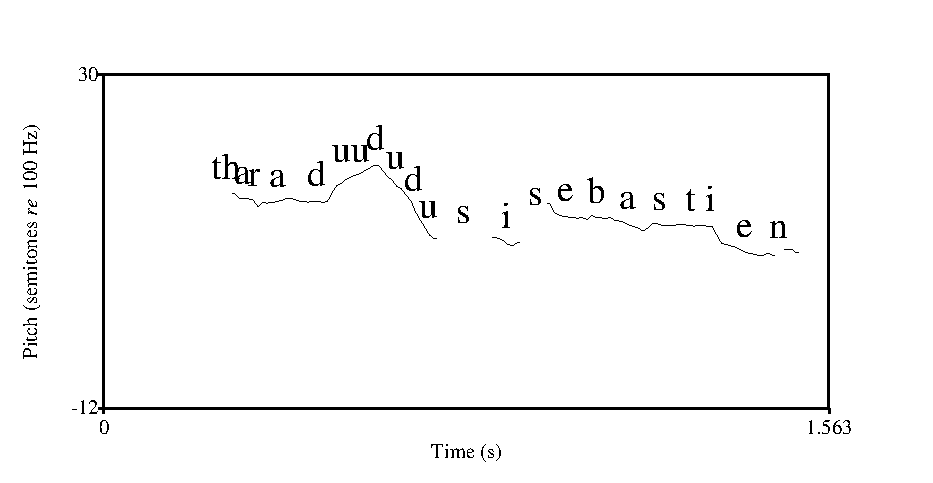
\includegraphics[width=0.5\textwidth]{./pics/tharaduudusisebastiennew.eps}
\glll ~~~~~~~~~~~H                   L ~ L\\
     thàrà-duudu=si $\mid$ Sebastian $\mid$  \\
     \textsc{neg.past}-stay=\textsc{interr} ~ Sebastian \\
    `You(=Sebastian) were not here, were you?'
\z
}
&\vspace{1cm}
 
 \textbf{Comment}: as above. The high tone of the assertional contour is linked to the beginning of the last lexical word, \trs{duuduk}{stay} in this case. The afterthought/anti-topic \citep{Chafe1976} \em Sebastian \em receives a new assertional intonation contour, but the pitch is not reset.\\
\end{tabular}



\begin{tabular}{lp{4cm}}\hspace{-1cm}
\xbox{12}{
\ea \label{ex:siithummabaapa}
 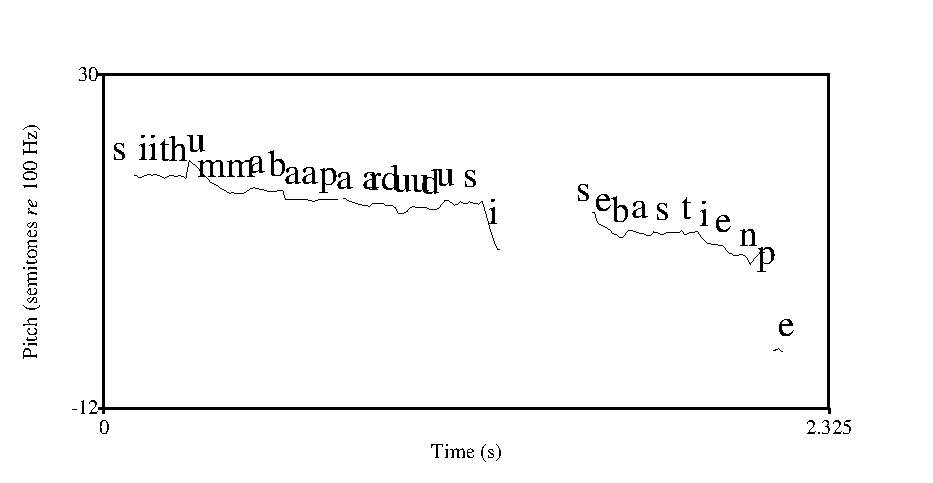
\includegraphics[width=0.5\textwidth]{./pics/siithummabaapaarduudusisebastianpenew.eps}
\glll ~       ~   ~          ~          L ~           L\\
    SLM1: siithu mma-baapa arà-duudu=si $\mid$ Sebastian=pe $\mid$ \\
    {} there mother-father \textsc{non.past}-stay=\textsc{interr} ~ Sebastian=\textsc{poss}   \\
    `Do your parents live there (i.e. Europe), Sebastian?' 
\z
}
&\vspace{1cm}
 
 \textbf{Comment}: In contrast to the preceding question, the afterthought \em Sebastian=pe \em is located in the same contour. The rather strong fall compared to the previous questions indicates security that my parents do indeed live there and reinforces the reading as a request for confirmation, rather than information.\\
\end{tabular}

\glossSTDmode
\begin{tabular}{lp{4cm}}\hspace{-1cm}
\xbox{12}{
\ea 
\gll SN: siithu?  \\
     {} there  \\
    `What do you mean by ``there''?' 
\z
} 
&\vspace{1cm}
 \textbf{Comment}: No intonation is given for the speech of the non-native variety spoken by the German researcher in order to avoid false conclusions drawn from this learner's phonology.\\
\end{tabular}

\glossINTmode
\begin{tabular}{lp{4cm}}\hspace{-1cm}
\xbox{12}{
\ea \label{ex:netherlandka}
 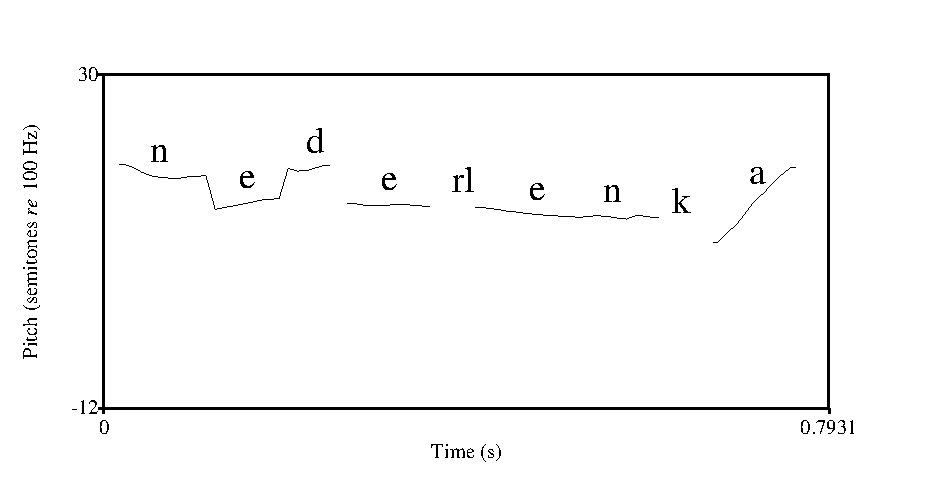
\includegraphics[width=0.5\textwidth]{./pics/nederlenkanew.eps}
\glll ~   ~~~~~~~~~~~~~~L H\\
     SLM1: {\em Netherland}=ka $\mid$?  \\
     {} Netherlands=\textsc{loc}  \\
    `Do they live in the Netherlands?' 
\z
}
&\vspace{1cm}
 \textbf{Comment}: Because the confirmation is declined, the question is restated, but with  a clear contour of request for information. \\
\end{tabular}

\glossSTDmode
\xbox{12}{
\ea 
\gll SN: {\em Germany}=ka.   \\
     {} Germany=\textsc{loc}  \\
    `They live in Germany.' 
\z
}\\

\glossINTmode
\begin{tabular}{lp{4cm}}\hspace{-1cm}
\xbox{12}{
\ea \label{ex:germanyka}
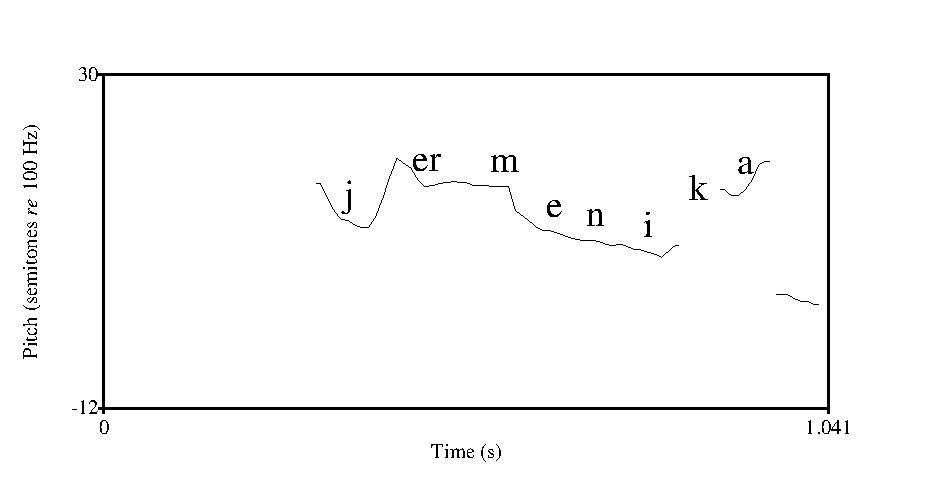
\includegraphics[width=0.5\textwidth]{./pics/jermenikanew.eps}
\glll ~    ~~H~~~~~~~~L H\\
     SLM1: {\em Germany}=ka $\mid$ \\
     {} Germany=\textsc{loc}  \\
    `Oh, so they live in Germany?' 
\z
}
&\vspace{1cm}
 
 \textbf{Comment}:Again a request for information, but less salient than the preceding one.  It indicates the surprise that members of my family live in separate countries, and requests confirmation of the veracity of that information. \em =si \em is not present.\\
\end{tabular}

\glossSTDmode
\xbox{12}{
 \ea 
\gll SN: {\em Germany}=ka.  \\
     {} Germany=\textsc{loc} \\
    `Yes, they live in Germany.' 
\z
}\\

\glossINTmode
\begin{tabular}{lp{4cm}}\hspace{-1cm}
\xbox{12}{
\ea \label{ex:sebastianaraduudukgermanyka}
\includegraphics[width=0.5\textwidth]{./pics/sebastianaraduudukjermannew.eps}
\glll ~  ~ ~ ~H L\\
      SLM1: Sebastian arà-duuduk {\em German} $\mid$.\\
     {} Sebastian \textsc{non.past}-stay Germany\\
    `So you live in Germany.'
\z
}
&\vspace{1cm}
 
 \textbf{Comment}: A tentative conclusion with a slight assertional contour. Listening to the example gives an impression of hesitation. The tentative conclusion seems to be `If the parents live in Germany, so must the son.'\\
\end{tabular}

\glossSTDmode
\xbox{12}{
\ea 
\gll   SN: no se se=jo {\em Netherlands}=ka,  se=ppe mma-baapa  {\em Germany}=ka   \\
       {} (no) \textsc{1s} \textsc{1s}=\textsc{emph} Netherlands=\textsc{loc}, \textsc{1s}=\textsc{poss} mother-father Germany=\textsc{loc} \\
    `No, \underline{I} live in the Netherlands, my parents live in Germany.'
\z
}\\

\glossINTmode
\begin{tabular}{lp{4cm}}\hspace{-1cm}
\xbox{12}{
\ea \label{ex:deranggermanyka}
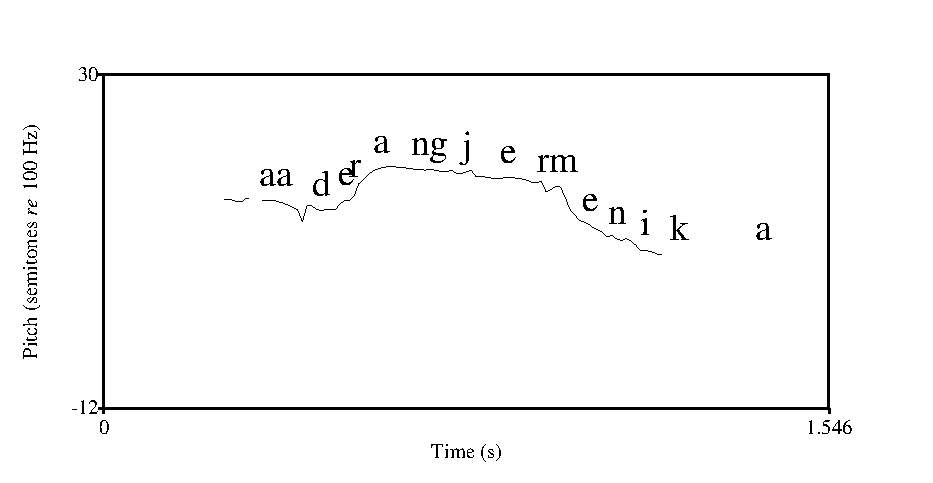
\includegraphics[width=0.5\textwidth]{./pics/aaderangjemernikanew.eps}
\glll  ~ ~~~~~~~H ~~H L\\
      SLM1: derang {\em Germany}=ka $\mid$ \\
     {} 3p Germany=\textsc{loc}.  \\
    `So they are in Germany.' 
\z
}
&\vspace{1cm}
 
 \textbf{Comment}: The solution of the mystery of parents and son living in different countries receives an assertional contour.\\
\end{tabular}

\begin{tabular}{lp{4cm}}\hspace{-1cm}
\xbox{12}{
\ea \label{ex:sudaarasudaari}
\includegraphics[width=0.5\textwidth]{./pics/sudaarasudaaripadanew.eps}
\glll ~          ~          ~     ~ ~             H\\
     SLM4: sudaara sudaari pada arà-duuduk=si $\mid$ \\
     {} brothers sisters \textsc{pl} \textsc{non.past}-be=\textsc{interr}  \\
    `Do you have brothers or sisters?'
\z
}
&\vspace{1cm}
 \textbf{Comment}: A new topic: siblings. The contour is a request for information with a rising pitch since there are no presumptions  available.\\
\end{tabular}

\glossSTDmode
\xbox{12}{
\ea 
\gll SN: {\em Germany}=ka duuva aade prompang aada  \\
     {} Germany=\textsc{loc} two younger.sibling woman exist  \\
    `I have two younger sisters who live in Germany' 
\z
}\\

\glossINTmode
\begin{tabular}{lp{4cm}}\hspace{-1cm}
\xbox{12}{
\ea 
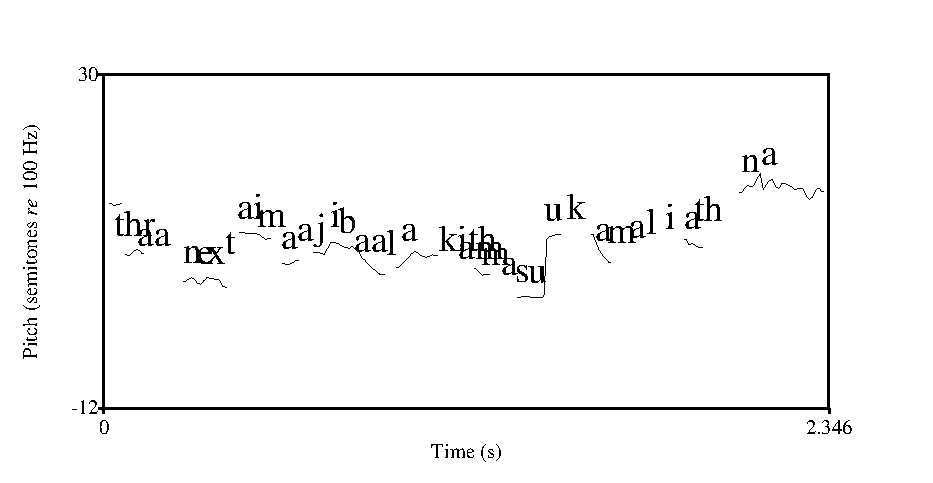
\includegraphics[width=0.5\textwidth]{./pics/nexttimeaajibanew.eps}
\glll ~       ~  ~    ~   H       ~~~H~~L  H     ~        ~ ~ H\\
     SLM5: thraa. next time $\mid$ aajibaa-la $\mid$ kithan=na suuka mà-liiyath-na $\mid$\\
     {} no next time ~  bring-\textsc{imp} ~ \textsc{1pl}=\textsc{dat} like \textsc{inf}-see-\textsc{dat}  \\
    `So bring them next time, we would like to see them (won't you)' 
\z
} 
&\vspace{1cm}
 \textbf{Comment}: This contour is difficult to interpret from pitch movement alone, but auditory impressions make it clear that we are dealing with a command. The rising pitch at the end might indicate mitigation, but this is unclear as of yet.\\
\end{tabular}

\begin{tabular}{lp{4cm}}\hspace{-1cm}
\xbox{12}{
\ea \label{ex:fotopadathraa}
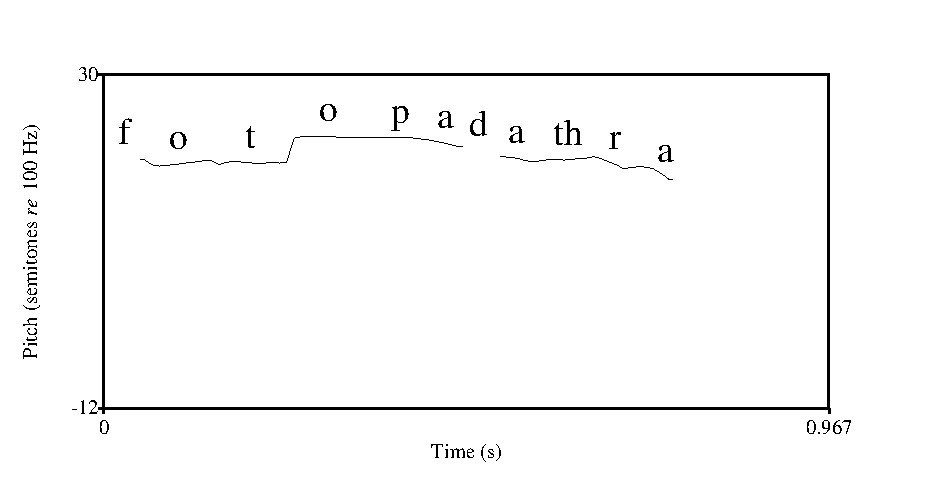
\includegraphics[width=0.5\textwidth]{./pics/fotopadathraanew.eps}
\glll   ~  ~~~H    ~    ~ L\\
       SLM2: {\em photo} pada thraa $\mid$ \\
     {} photo \textsc{pl}  \textsc{neg}.exist\\
    `You have no photos?' 
\z
}
&\vspace{1cm}
 
 \textbf{Comment}: Again a new topic, but with the underlying assumption that I have indeed not brought any photos: assertional contour. Note the absence of the clitic \em =si \em despite the question illocution.\\
\end{tabular}

\glossSTDmode
\begin{tabular}{lp{4cm}}\hspace{-1cm}
\xbox{12}{
\ea \label{ex:fotopadathraasi}
\gll SLM1: {\em photo} pada thraa=si \\
     {} photo \textsc{pl}  \textsc{neg}.exist=\textsc{interr}\\
    `You have no photos, have you?' 
\z
}
&\vspace{1cm}
\textbf{Comment}: No analysis due to problems with the sound file. (Multiple speakers at the same time, background noise)\\
\end{tabular}

\begin{tabular}{lp{4cm}}\hspace{-1cm}
\xbox{12}{
\ea 
\gll SLM6: gaa\u mbar gaa\u mbar. \\
     {} ``gaa\u mbar'' ``gaa\u mbar''.  \\
    `The word is ``gaa\u mbar''.
\z
}
&\vspace{1cm}

\textbf{Comment}: No analysis due to problems with the sound file\\
\end{tabular}

\begin{tabular}{lp{4cm}}\hspace{-1cm}
\xbox{12}{
\ea 
\gll  SLM1: thraa, thraa\\
      {} \textsc{neg}.exist, \textsc{neg}.exist\\
    `No, he has no photos.' 
\z
}
&\vspace{1cm}

\textbf{Comment}: No analysis due to problems with the sound file\\
\end{tabular}

\begin{tabular}{lp{4cm}}\hspace{-1cm}
\xbox{12}{
\ea \label{ex:sebastianskaaving}
\gll SLM3: Sebastian s-kaaving?   \\
     {} Sebastian \textsc{cp}-marry  \\
    `Is Sebastian married.' (asking other women)
\z
}
&\vspace{1cm}

\textbf{Comment}: No analysis due to problems with the sound file\\
\end{tabular}

\glossINTmode
\begin{tabular}{lp{4cm}}\hspace{-1cm}
\xbox{12}{
\ea \label{ex:sebastianthamakaavingsi}
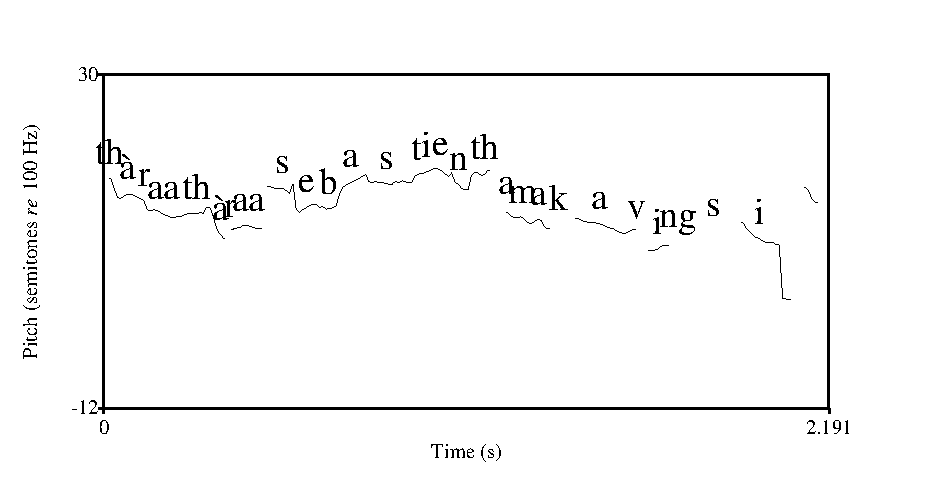
\includegraphics[width=0.5\textwidth]{./pics/sebastianthamakaavingnew.eps}
\glll ~       ~  ~       L     ~          H     H              L\\
     SLM1: thàra thàra $\mid$ Sebastian $\mid$ thama-kaaving=si $\mid$  \\
     {} no no ~ Sebastian ~ \textsc{neg.nonpast}-marry=\textsc{interr}  \\
    `You are not married, are you?' 
\z
}
&\vspace{1cm}
 
 \textbf{Comment}:The presupposition is that I am not married. The overall contour is assertional, a request for confirmation. The very slight rise at the end indicates a remainder of doubt (cf. \xref{ex:fotopadathraa}).\\
\end{tabular}


\begin{tabular}{lp{4cm}}\hspace{-1cm}
\xbox{12}{
 \ea \label{ex:srilankakajokaaving}
\includegraphics[width=0.5\textwidth]{./pics/srilankakajokaavingnew.eps}
\glll ~      ~   ~          H ~     L\\
     SLM1: Sri Lanka=ka=jo $\mid$ kaving  $\mid$ \\
     {} Sri Lanka=\textsc{loc}=\textsc{emph} ~ marry  \\
    `Marry in Sri Lanka!' 
\z
}
&\vspace{1cm}
 
 \textbf{Comment}:A jocular imperative. The high tone is located at the end of the argument phrase/the beginning of the predicate phrase (The plateau around the second k is an artefact.)\\
\end{tabular}

\glossSTDmode

% Short and long vowels can be distinguished phonetically in SLM. Long vowels can only be found in the penultimate syllable of disyllables and of trisyllables with a schwa in the first syllable. \citet{Bichsel} and \citet{SmithEtAl2004} argue that vowel length is phonemic, while \citet{Tapovanaye1995} argues that it is a function of syllable structure. The vowel is used to contribute an extra mora required by word structure. In Section \ref{sec:phon:wordstructure} we will show that vowel length can indeed be predicted on the basis of word structure and is thus not phonemic.
